% !TeX spellcheck = hu_HU
% !TeX encoding = UTF-8
% !TeX program = xelatex
\documentclass[11pt,a4paper,oneside]{report}             % Single-side
%\documentclass[11pt,a4paper,twoside,openright]{report}  % Duplex

% thanks to http://tex.stackexchange.com/a/47579/71109
\usepackage{pdfpages}
\usepackage{ifxetex}
\usepackage{ifluatex}
\newif\ifxetexorluatex % a new conditional starts as false
\ifnum 0\ifxetex 1\fi\ifluatex 1\fi>0
   \xetexorluatextrue
\fi

\ifxetexorluatex
  \usepackage{fontspec}
\else
  \usepackage[T1]{fontenc}
  \usepackage[utf8]{inputenc}
  \usepackage[lighttt]{lmodern}
\fi

\usepackage[english,magyar]{babel} % Alapértelmezés szerint utoljára definiált nyelv lesz aktív, de később külön beállítjuk az aktív nyelvet.

%\usepackage{cmap}
\usepackage{amsfonts,amsmath,amssymb} % Mathematical symbols.
%\usepackage[ruled,boxed,resetcount,linesnumbered]{algorithm2e} % For pseudocodes. % beware: this is not compatible with LuaLaTeX, see http://tex.stackexchange.com/questions/34814/lualatex-and-algorithm2e
\usepackage{booktabs} % For publication quality tables for LaTeX
\usepackage{graphicx}

%\usepackage{fancyhdr}
%\usepackage{lastpage}

\usepackage{anysize}
%\usepackage{sectsty}
\usepackage{setspace} % For setting line spacing

\usepackage[unicode]{hyperref} % For hyperlinks in the generated document.
%\usepackage{xcolor} maybe have to use this later
\usepackage{listings} % For source code snippets.
\usepackage{float}
\usepackage[table,xcdraw]{xcolor}

\usepackage[amsmath,thmmarks]{ntheorem} % Theorem-like environments.

\usepackage[hang]{caption}

\singlespacing

\newcommand{\selecthungarian}{
	\selectlanguage{magyar}
	\setlength{\parindent}{2em}
	\setlength{\parskip}{0em}
	\frenchspacing
}

\newcommand{\selectenglish}{
	\selectlanguage{english}
	\setlength{\parindent}{0em}
	\setlength{\parskip}{0.5em}
	\nonfrenchspacing
	\renewcommand{\figureautorefname}{Figure}
	\renewcommand{\tableautorefname}{Table}
	\renewcommand{\partautorefname}{Part}
	\renewcommand{\chapterautorefname}{Chapter}
	\renewcommand{\sectionautorefname}{Section}
	\renewcommand{\subsectionautorefname}{Section}
	\renewcommand{\subsubsectionautorefname}{Section}
}

\usepackage[numbers]{natbib}
\usepackage{xspace}


\newcommand{\vikszerzoVezeteknev}{Varga}
\newcommand{\vikszerzoKeresztnev}{Dominik}

\newcommand{\vikkonzulensAVezeteknev}{Raikovich}
\newcommand{\vikkonzulensAKeresztnev}{Tamás}

\newcommand{\vikcim}{A NES videojáték konzol FPGA alapú megvalósítása} % Cím
\newcommand{\viktanszek}{\bmemit} % Tanszék
\newcommand{\vikdoktipus}{\msc} % Dokumentum típusa (\bsc vagy \msc)
\newcommand{\vikmunkatipusat}{diplomatervet} % a "hallgató nyilatkozat" részhez: szakdolgozatot vagy diplomatervet

\newcommand{\szerzoMeta}{\vikszerzoVezeteknev{} \vikszerzoKeresztnev} % egy szerző esetén
%\newcommand{\szerzoMeta}{\vikszerzoVezeteknev{} \vikszerzoKeresztnev, \tdkszerzoB} % két szerző esetén

% Beállítások magyar nyelvű dolgozathoz
%--------------------------------------------------------------------------------------
% Elnevezések
%--------------------------------------------------------------------------------------
\newcommand{\bme}{Budapesti Műszaki és Gazdaságtudományi Egyetem}
\newcommand{\vik}{Villamosmérnöki és Informatikai Kar}

\newcommand{\bmemit}{Méréstechnika és Információs Rendszerek Tanszék}

\newcommand{\keszitette}{Készítette}
\newcommand{\konzulens}{Konzulens}

\newcommand{\bsc}{Szakdolgozat}
\newcommand{\msc}{Diplomaterv}
\newcommand{\tdk}{TDK dolgozat}
\newcommand{\bsconlab}{BSc Önálló laboratórium}
\newcommand{\msconlabi}{MSc Önálló laboratórium 1.}
\newcommand{\msconlabii}{MSc Önálló laboratórium 2.}

\newcommand{\pelda}{Példa}
\newcommand{\definicio}{Definíció}
\newcommand{\tetel}{Tétel}

\newcommand{\bevezetes}{Bevezetés}
\newcommand{\koszonetnyilvanitas}{Köszönetnyilvánítás}
\newcommand{\fuggelek}{Függelék}

% Opcionálisan átnevezhető címek
%\addto\captionsmagyar{
%\renewcommand{\listfigurename}{ábra:}
%\renewcommand{\listtablename}{táblázat:}
%\renewcommand{\bibname}{Saját irodalomjegyzék név}
%}

\newcommand{\szerzo}{\vikszerzoVezeteknev{} \vikszerzoKeresztnev}
\newcommand{\vikkonzulensA}{\vikkonzulensAVezeteknev{} \vikkonzulensAKeresztnev}

\newcommand{\selectthesislanguage}{\selecthungarian}

\bibliographystyle{huplain}

%\addto\captionsmagyar{\renewcommand{\figurename}{ábra:}}

%\addto\captionsmagyar{
%\renewcommand{\thefigure}{.}
%\renewcommand{\figurename}{ábra}
%}

\def\lstlistingname{hardverleírás részlet}

\newcommand{\appendixnumber}{6}  % a fofejezet-szamlalo az angol ABC 6. betuje (F) lesz

% Settings for English documents
%%--------------------------------------------------------------------------------------
% Elnevezések
%--------------------------------------------------------------------------------------
\newcommand{\bme}{Budapest University of Technology and Economics}
\newcommand{\vik}{Faculty of Electrical Engineering and Informatics}

\newcommand{\bmemit}{Department of Measurement and Information Systems}

\newcommand{\keszitette}{Author}
\newcommand{\konzulens}{Advisor}

\newcommand{\bsc}{Bachelor's Thesis}
\newcommand{\msc}{Master's Thesis}
\newcommand{\tdk}{Scientific Students' Association Report}
\newcommand{\bsconlab}{BSc Project Laboratory}
\newcommand{\msconlabi}{MSc Project Laboratory 1}
\newcommand{\msconlabii}{MSc Project Laboratory 2}

\newcommand{\pelda}{Example}
\newcommand{\definicio}{Definition}
\newcommand{\tetel}{Theorem}

\newcommand{\bevezetes}{Introduction}
\newcommand{\koszonetnyilvanitas}{Acknowledgements}
\newcommand{\fuggelek}{Appendix}

% Optional custom titles
%\addto\captionsenglish{%
%\renewcommand*{\listfigurename}{Your list of figures title}
%\renewcommand*{\listtablename}{Your list of tables title}
%\renewcommand*{\bibname}{Your bibliography title}
%}

\newcommand{\szerzo}{\vikszerzoKeresztnev{} \vikszerzoVezeteknev}
\newcommand{\vikkonzulensA}{\vikkonzulensAMegszolitas\vikkonzulensAKeresztnev{} \vikkonzulensAVezeteknev}
\newcommand{\vikkonzulensB}{\vikkonzulensBMegszolitas\vikkonzulensBKeresztnev{} \vikkonzulensBVezeteknev}
\newcommand{\vikkonzulensC}{\vikkonzulensCMegszolitas\vikkonzulensCKeresztnev{} \vikkonzulensCVezeteknev}

\newcommand{\selectthesislanguage}{\selectenglish}

\bibliographystyle{plainnat}

\newcommand{\ie}{i.e.\@\xspace}
\newcommand{\Ie}{I.e.\@\xspace}
\newcommand{\eg}{e.g.\@\xspace}
\newcommand{\Eg}{E.g.\@\xspace}
\newcommand{\etal}{et al.\@\xspace}
\newcommand{\etc}{etc.\@\xspace}
\newcommand{\vs}{vs.\@\xspace}
\newcommand{\viz}{viz.\@\xspace} % videlicet
\newcommand{\cf}{cf.\@\xspace} % confer
\newcommand{\Cf}{Cf.\@\xspace}
\newcommand{\wrt}{w.r.t.\@\xspace} % with respect to
\newcommand{\approximately}{approx.\@\xspace}

\newcommand{\appendixnumber}{1}  % a fofejezet-szamlalo az angol ABC 1. betuje (A) lesz


%--------------------------------------------------------------------------------------
% Page layout setup
%--------------------------------------------------------------------------------------
% we need to redefine the pagestyle plain
% another possibility is to use the body of this command without \fancypagestyle
% and use \pagestyle{fancy} but in that case the special pages
% (like the ToC, the References, and the Chapter pages)remain in plane style

\pagestyle{plain}
\marginsize{35mm}{25mm}{15mm}{15mm}

\setcounter{tocdepth}{3}
%\sectionfont{\large\upshape\bfseries}
\setcounter{secnumdepth}{3}

\usepackage[labelsep=colon]{caption}

\sloppy % Margón túllógó sorok tiltása.
\widowpenalty=10000 \clubpenalty=10000 %A fattyú- és árvasorok elkerülése
\def\hyph{-\penalty0\hskip0pt\relax} % Kötőjeles szavak elválasztásának engedélyezése


%--------------------------------------------------------------------------------------
% Setup hyperref package
%--------------------------------------------------------------------------------------
\hypersetup{
    % bookmarks=true,            % show bookmarks bar?
    unicode=true,              % non-Latin characters in Acrobat's bookmarks
    pdftitle={\vikcim},        % title
    pdfauthor={\szerzoMeta},    % author
    pdfsubject={\vikdoktipus}, % subject of the document
    pdfcreator={\szerzoMeta},   % creator of the document
    pdfproducer={},    % producer of the document
    pdfkeywords={},    % list of keywords (separate then by comma)
    pdfnewwindow=true,         % links in new window
    colorlinks=true,           % false: boxed links; true: colored links
    linkcolor=black,           % color of internal links
    citecolor=black,           % color of links to bibliography
    filecolor=black,           % color of file links
    urlcolor=black             % color of external links
}


%--------------------------------------------------------------------------------------
% Set up listings
%--------------------------------------------------------------------------------------
\definecolor{lightgray}{rgb}{0.95,0.95,0.95}
\lstset{
	basicstyle=\scriptsize\ttfamily, % print whole listing small
	keywordstyle=\color{black}\bfseries, % bold black keywords
	identifierstyle=, % nothing happens
	% default behavior: comments in italic, to change use
	% commentstyle=\color{green}, % for e.g. green comments
	stringstyle=\scriptsize,
	showstringspaces=false, % no special string spaces
	aboveskip=3pt,
	belowskip=3pt,
	backgroundcolor=\color{lightgray},
	columns=flexible,
	keepspaces=true,
	escapeinside={(*@}{@*)},
	captionpos=b,
	breaklines=true,
	frame=single,
	float=!ht,
	tabsize=2,
	literate=*
		{á}{{\'a}}1	{é}{{\'e}}1	{í}{{\'i}}1	{ó}{{\'o}}1	{ö}{{\"o}}1	{ő}{{\H{o}}}1	{ú}{{\'u}}1	{ü}{{\"u}}1	{ű}{{\H{u}}}1
		{Á}{{\'A}}1	{É}{{\'E}}1	{Í}{{\'I}}1	{Ó}{{\'O}}1	{Ö}{{\"O}}1	{Ő}{{\H{O}}}1	{Ú}{{\'U}}1	{Ü}{{\"U}}1	{Ű}{{\H{U}}}1
}

%--------------------------------------------------------------------------------------
% Verilog Code Style
%--------------------------------------------------------------------------------------
\definecolor{verilogcommentcolor}{RGB}{104,180,104}
\definecolor{verilogkeywordcolor}{RGB}{49,49,255}
\definecolor{verilogsystemcolor}{RGB}{128,0,255}
\definecolor{verilognumbercolor}{RGB}{255,143,102}
\definecolor{verilogstringcolor}{RGB}{160,160,160}
\definecolor{verilogdefinecolor}{RGB}{128,64,0}
\definecolor{verilogoperatorcolor}{RGB}{0,0,128}

% Verilog style
\lstdefinestyle{prettyverilog}{
	language           = Verilog,
	commentstyle       = \color{verilogcommentcolor},
	alsoletter         = \$'0123456789\`,
	literate           = *{+}{{\verilogColorOperator{+}}}{1}%
	{-}{{\verilogColorOperator{-}}}{1}%
	{@}{{\verilogColorOperator{@}}}{1}%
	{;}{{\verilogColorOperator{;}}}{1}%
	{*}{{\verilogColorOperator{*}}}{1}%
	{?}{{\verilogColorOperator{?}}}{1}%
	{:}{{\verilogColorOperator{:}}}{1}%
	{<}{{\verilogColorOperator{<}}}{1}%
	{>}{{\verilogColorOperator{>}}}{1}%
	{=}{{\verilogColorOperator{=}}}{1}%
	{!}{{\verilogColorOperator{!}}}{1}%
	{^}{{\verilogColorOperator{$\land$}}}{1}%
	{|}{{\verilogColorOperator{|}}}{1}%
	{=}{{\verilogColorOperator{=}}}{1}%
	{[}{{\verilogColorOperator{[}}}{1}%
	{]}{{\verilogColorOperator{]}}}{1}%
	{(}{{\verilogColorOperator{(}}}{1}%
	{)}{{\verilogColorOperator{)}}}{1}%
	{,}{{\verilogColorOperator{,}}}{1}%
	{.}{{\verilogColorOperator{.}}}{1}%
	{~}{{\verilogColorOperator{$\sim$}}}{1}%
	{\%}{{\verilogColorOperator{\%}}}{1}%
	{\&}{{\verilogColorOperator{\&}}}{1}%
	{\#}{{\verilogColorOperator{\#}}}{1}%
	{\ /\ }{{\verilogColorOperator{\ /\ }}}{3}%
	{\ _}{\ \_}{2}%
	,
	morestring         = [s][\color{verilogstringcolor}]{"}{"},%
	identifierstyle    = \color{black},
	vlogdefinestyle    = \color{verilogdefinecolor},
	vlogconstantstyle  = \color{verilognumbercolor},
	vlogsystemstyle    = \color{verilogsystemcolor},
	basicstyle         = \scriptsize\fontencoding{T1}\ttfamily,
	keywordstyle       = \bfseries\color{verilogkeywordcolor},
	numbers            = left,
	numbersep          = 10pt,
	tabsize            = 4,
	escapeinside       = {/*!}{!*/},
	upquote            = true,
	sensitive          = true,
	showstringspaces   = false, %without this there will be a symbol in the places where there is a space
	frame              = single
}


% This is shamelessly stolen and modified from:
% https://github.com/jubobs/sclang-prettifier/blob/master/sclang-prettifier.dtx
\makeatletter

% Language name
\newcommand\language@verilog{Verilog}
\expandafter\lst@NormedDef\expandafter\languageNormedDefd@verilog%
\expandafter{\language@verilog}

% save definition of single quote for testing
\lst@SaveOutputDef{`'}\quotesngl@verilog
\lst@SaveOutputDef{``}\backtick@verilog
\lst@SaveOutputDef{`\$}\dollar@verilog

% Extract first character token in sequence and store in macro 
% firstchar@verilog, per http://tex.stackexchange.com/a/159267/21891
\newcommand\getfirstchar@verilog{}
\newcommand\getfirstchar@@verilog{}
\newcommand\firstchar@verilog{}
\def\getfirstchar@verilog#1{\getfirstchar@@verilog#1\relax}
\def\getfirstchar@@verilog#1#2\relax{\def\firstchar@verilog{#1}}

% Initially empty hook for lst
\newcommand\addedToOutput@verilog{}
\lst@AddToHook{Output}{\addedToOutput@verilog}

% The style used for constants as set in lstdefinestyle
\newcommand\constantstyle@verilog{}
\lst@Key{vlogconstantstyle}\relax%
{\def\constantstyle@verilog{#1}}

% The style used for defines as set in lstdefinestyle
\newcommand\definestyle@verilog{}
\lst@Key{vlogdefinestyle}\relax%
{\def\definestyle@verilog{#1}}

% The style used for defines as set in lstdefinestyle
\newcommand\systemstyle@verilog{}
\lst@Key{vlogsystemstyle}\relax%
{\def\systemstyle@verilog{#1}}

% Counter used to check current character is a digit
\newcount\currentchar@verilog

% Processing macro
\newcommand\@ddedToOutput@verilog
{%
	% If we're in \lstpkg{}' processing mode...
	\ifnum\lst@mode=\lst@Pmode%
	% Save the first token in the current identifier to \@getfirstchar
	\expandafter\getfirstchar@verilog\expandafter{\the\lst@token}%
	% Check if the token is a backtick
	\expandafter\ifx\firstchar@verilog\backtick@verilog
	% If so, then this starts a define
	\let\lst@thestyle\definestyle@verilog%
	\else
	% Check if the token is a dollar
	\expandafter\ifx\firstchar@verilog\dollar@verilog
	% If so, then this starts a system command
	\let\lst@thestyle\systemstyle@verilog%
	\else
	% Check if the token starts with a single quote
	\expandafter\ifx\firstchar@verilog\quotesngl@verilog
	% If so, then this starts a constant without length
	\let\lst@thestyle\constantstyle@verilog%
	\else
	\currentchar@verilog=48
	\loop
	\expandafter\ifnum%
	\expandafter`\firstchar@verilog=\currentchar@verilog%
	\let\lst@thestyle\constantstyle@verilog%
	\let\iterate\relax%
	\fi
	\advance\currentchar@verilog by \@ne%
	\unless\ifnum\currentchar@verilog>57%
	\repeat%
	\fi
	\fi
	\fi
	% ...but override by keyword style if a keyword is detected!
	%\lsthk@DetectKeywords% 
	\fi
}

% Add processing macro only if verilog
\lst@AddToHook{PreInit}{%
	\ifx\lst@language\languageNormedDefd@verilog%
	\let\addedToOutput@verilog\@ddedToOutput@verilog%
	\fi
}

% Colour operators in literate
\newcommand{\verilogColorOperator}[1]
{%
	\ifnum\lst@mode=\lst@Pmode\relax%
	{\bfseries\textcolor{verilogoperatorcolor}{#1}}%
	\else
	#1%
	\fi
}

\makeatother
%--------------------------------------------------------------------------------------
% End Verilog Code Style
%--------------------------------------------------------------------------------------

%--------------------------------------------------------------------------------------
% Set up theorem-like environments
%--------------------------------------------------------------------------------------
% Using ntheorem package -- see http://www.math.washington.edu/tex-archive/macros/latex/contrib/ntheorem/ntheorem.pdf

\theoremstyle{plain}
\theoremseparator{.}
\newtheorem{example}{\pelda}

\theoremseparator{.}
%\theoremprework{\bigskip\hrule\medskip}
%\theorempostwork{\hrule\bigskip}
\theorembodyfont{\upshape}
\theoremsymbol{{\large \ensuremath{\centerdot}}}
\newtheorem{definition}{\definicio}

\theoremseparator{.}
%\theoremprework{\bigskip\hrule\medskip}
%\theorempostwork{\hrule\bigskip}
\newtheorem{theorem}{\tetel}


%--------------------------------------------------------------------------------------
% Some new commands and declarations
%--------------------------------------------------------------------------------------
\newcommand{\code}[1]{{\upshape\ttfamily\scriptsize\indent #1}}
\newcommand{\doi}[1]{DOI: \href{http://dx.doi.org/\detokenize{#1}}{\raggedright{\texttt{\detokenize{#1}}}}} % A hivatkozások közt így könnyebb DOI-t megadni.

\DeclareMathOperator*{\argmax}{arg\,max}
%\DeclareMathOperator*[1]{\floor}{arg\,max}
\DeclareMathOperator{\sign}{sgn}
\DeclareMathOperator{\rot}{rot}


%--------------------------------------------------------------------------------------
% Setup captions
%--------------------------------------------------------------------------------------
\captionsetup[figure]{
	width=.75\textwidth,
	aboveskip=10pt}

\renewcommand{\captionlabelfont}{\bf}
%\renewcommand{\captionfont}{\footnotesize\it}

%--------------------------------------------------------------------------------------
% Hyphenation exceptions
%--------------------------------------------------------------------------------------
\hyphenation{Shakes-peare Mar-seilles ár-víz-tű-rő tü-kör-fú-ró-gép}

%--------------------------------------------------------------------------------------
% Table float box with bottom caption, box width adjusted to content
%--------------------------------------------------------------------------------------



\author{\vikszerzo}
\title{\viktitle}

%--------------------------------------------------------------------------------------
% Table of contents and the main text
%--------------------------------------------------------------------------------------
\begin{document}

\pagenumbering{gobble}

%TODO These includes define guidelines -- remove these
%~~~~~~~~~~~~~~~~~~~~~~~~~~~~~~~~~~~~~~~~~~~~~~~~~~~~~~~~~~~~~~~~~~~~~~~~~~~~~~~~~~~~~~
%\selecthungarian
%--------------------------------------------------------------------------------------
% Rovid formai es tartalmi tajekoztato
%--------------------------------------------------------------------------------------

\footnotesize
\begin{center}
\large
\textbf{\Large Általános információk, a diplomaterv szerkezete}\\
\end{center}

A diplomaterv szerkezete a BME Villamosmérnöki és Informatikai Karán:
\begin{enumerate}
\item	Diplomaterv feladatkiírás
\item	Címoldal
\item	Tartalomjegyzék
\item	A diplomatervező nyilatkozata az önálló munkáról és az elektronikus adatok kezeléséről
\item	Tartalmi összefoglaló magyarul és angolul
\item	Bevezetés: a feladat értelmezése, a tervezés célja, a feladat indokoltsága, a diplomaterv felépítésének rövid összefoglalása
\item	A feladatkiírás pontosítása és részletes elemzése
\item	Előzmények (irodalomkutatás, hasonló alkotások), az ezekből levonható következtetések
\item	A tervezés részletes leírása, a döntési lehetőségek értékelése és a választott megoldások indoklása
\item	A megtervezett műszaki alkotás értékelése, kritikai elemzése, továbbfejlesztési lehetőségek
\item	Esetleges köszönetnyilvánítások
\item	Részletes és pontos irodalomjegyzék
\item	Függelék(ek)
\end{enumerate}

Felhasználható a következő oldaltól kezdődő \LaTeX diplomatervsablon dokumentum tartalma. 

A diplomaterv szabványos méretű A4-es lapokra kerüljön. Az oldalak tükörmargóval készüljenek (mindenhol 2,5~cm, baloldalon 1~cm-es kötéssel). Az alapértelmezett betűkészlet a 12 pontos Times New Roman, másfeles sorközzel, de ettől kismértékben el lehet térni, ill. más betűtípus használata is megengedett.

Minden oldalon -- az első négy szerkezeti elem kivételével -- szerepelnie kell az oldalszámnak.

A fejezeteket decimális beosztással kell ellátni. Az ábrákat a megfelelő helyre be kell illeszteni, fejezetenként decimális számmal és kifejező címmel kell ellátni. A fejezeteket decimális aláosztással számozzuk, maximálisan 3 aláosztás mélységben (pl. 2.3.4.1.). Az ábrákat, táblázatokat és képleteket célszerű fejezetenként külön számozni (pl. 2.4. ábra, 4.2. táblázat vagy képletnél (3.2)). A fejezetcímeket igazítsuk balra, a normál szövegnél viszont használjunk sorkiegyenlítést. Az ábrákat, táblázatokat és a hozzájuk tartozó címet igazítsuk középre. A cím a jelölt rész alatt helyezkedjen el.

A képeket lehetőleg rajzoló programmal készítsék el, az egyenleteket egyenlet-szerkesztő segítségével írják le (A \LaTeX~ehhez kézenfekvő megoldásokat nyújt).

Az irodalomjegyzék szövegközi hivatkozása történhet sorszámozva (ez a preferált megoldás) vagy a Harvard-rendszerben (a szerző és az évszám megadásával). A teljes lista névsor szerinti sorrendben a szöveg végén szerepeljen (sorszámozott irodalmi hivatkozások esetén hivatkozási sorrendben). A szakirodalmi források címeit azonban mindig az eredeti nyelven kell megadni, esetleg zárójelben a fordítással. A listában szereplő valamennyi publikációra hivatkozni kell a szövegben (a \LaTeX-sablon a Bib\TeX~segítségével mindezt automatikusan kezeli). Minden publikáció a szerzők után a következő adatok szerepelnek: folyóirat cikkeknél a pontos cím, a folyóirat címe, évfolyam, szám, oldalszám tól-ig. A folyóiratok címét csak akkor rövidítsük, ha azok nagyon közismertek vagy nagyon hosszúak. Internetes hivatkozások megadásakor fontos, hogy az elérési út előtt megadjuk az oldal tulajdonosát és tartalmát (mivel a link egy idő után akár elérhetetlenné is válhat), valamint az elérés időpontját.

\vspace{5mm}
Fontos:
\begin{itemize}
	\item A szakdolgozatkészítő / diplomatervező nyilatkozata (a jelen sablonban szereplő szövegtartalommal) kötelező előírás, Karunkon ennek hiányában a szakdolgozat/diplomaterv nem bírálható és nem védhető!
	\item Mind a dolgozat, mind a melléklet maximálisan 15~MB méretű lehet!
\end{itemize}

\vspace{5mm}
\begin{center}
Jó munkát, sikeres szakdolgozatkészítést, ill. diplomatervezést kívánunk!
\end{center}

\normalsize
\selectthesislanguage

%--------------------------------------------------------------------------------------
% Feladatkiiras (a tanszeken atveheto, kinyomtatott valtozat)
%--------------------------------------------------------------------------------------
\clearpage
\begin{center}
\large
\textbf{FELADATKIÍRÁS}\\
\end{center}

A feladatkiírást a tanszéki adminisztrációban lehet átvenni, és a leadott munkába eredeti, tanszéki pecséttel ellátott és a tanszékvezető által aláírt lapot kell belefűzni (ezen oldal \emph{helyett}, ez az oldal csak útmutatás). Az elektronikusan feltöltött dolgozatban már nem kell beleszerkeszteni ezt a feladatkiírást.


\selectthesislanguage

%~~~~~~~~~~~~~~~~~~~~~~~~~~~~~~~~~~~~~~~~~~~~~~~~~~~~~~~~~~~~~~~~~~~~~~~~~~~~~~~~~~~~~~
\hypersetup{pageanchor=false}
%--------------------------------------------------------------------------------------
%	The title page
%--------------------------------------------------------------------------------------
\begin{titlepage}
\begin{center}

\includegraphics[width=60mm,keepaspectratio]{figures/bme_logo.pdf}\\
\vspace{0.3cm}
\textbf{\bme}\\
\textmd{\vik}\\
\textmd{\viktanszek}\\[5cm]

\vspace{0.4cm}
{\huge \bfseries \vikcim}\\[0.8cm]
\vspace{0.5cm}
\textsc{\Large \vikdoktipus}\\[4cm]

{
	\renewcommand{\arraystretch}{0.85}
	\begin{tabular}{cc}
	 \makebox[7cm]{\emph{\keszitette}} & \makebox[7cm]{\emph{\konzulens}} \\ \noalign{\smallskip}
	 \makebox[7cm]{\szerzo} & \makebox[7cm]{\vikkonzulensA} \\
	\end{tabular}
}

\vfill
{\large \today}
\end{center}
\end{titlepage}
\hypersetup{pageanchor=false}

		   % Szakdolgozat/Diplomaterv címlap
%\include{include/titlepage-tdk}	% TDK címlap
%\include{include/titlepage-otdk}   % OTDK címlap


% Table of Contents
%~~~~~~~~~~~~~~~~~~~~~~~~~~~~~~~~~~~~~~~~~~~~~~~~~~~~~~~~~~~~~~~~~~~~~~~~~~~~~~~~~~~~~~
\tableofcontents\vfill


% Declaration and Abstract
%~~~~~~~~~~~~~~~~~~~~~~~~~~~~~~~~~~~~~~~~~~~~~~~~~~~~~~~~~~~~~~~~~~~~~~~~~~~~~~~~~~~~~~
\selectlanguage{magyar}
\pagenumbering{gobble}
%--------------------------------------------------------------------------------------
% Nyilatkozat
%--------------------------------------------------------------------------------------
\begin{center}
\large
\textbf{HALLGATÓI NYILATKOZAT}\\
\end{center}

Alulírott \emph{\vikszerzoVezeteknev{} \vikszerzoKeresztnev}, szigorló hallgató kijelentem, hogy ezt a \vikmunkatipusat{} meg nem engedett segítség nélkül, saját magam készítettem, csak a megadott forrásokat (szakirodalom, eszközök stb.) használtam fel. Minden olyan részt, melyet szó szerint, vagy azonos értelemben, de átfogalmazva más forrásból átvettem, egyértelműen, a forrás megadásával megjelöltem.

Hozzájárulok, hogy a jelen munkám alapadatait (szerző(k), cím, angol és magyar nyelvű tartalmi kivonat, készítés éve, konzulens(ek) neve) a BME VIK nyilvánosan hozzáférhető elektronikus formában, a munka teljes szövegét pedig az egyetem belső hálózatán keresztül (vagy autentikált felhasználók számára) közzétegye. Kijelentem, hogy a benyújtott munka és annak elektronikus verziója megegyezik. Dékáni engedéllyel titkosított diplomatervek esetén a dolgozat szövege csak 3 év eltelte után válik hozzáférhetővé.

\begin{flushleft}
\vspace*{1cm}
Budapest, \today
\end{flushleft}

\begin{flushright}
 \vspace*{1cm}
 \makebox[7cm]{\rule{6cm}{.4pt}}\\
 \makebox[7cm]{\emph{\vikszerzoVezeteknev{} \vikszerzoKeresztnev}}\\
 \makebox[7cm]{hallgató}
\end{flushright}
\thispagestyle{empty}

\vfill
\clearpage
\thispagestyle{empty} % an empty page

\selectthesislanguage
 %TODO Hallgatói nyilatkozat
%\pagenumbering{roman}
\setcounter{page}{1}

\selecthungarian

%----------------------------------------------------------------------------
% Abstract in Hungarian
%----------------------------------------------------------------------------
\chapter*{Kivonat}\addcontentsline{toc}{chapter}{Kivonat}

Jelen dokumentum egy diplomaterv sablon, amely formai keretet ad a BME Villamosmérnöki és Informatikai Karán végző hallgatók által elkészítendő szakdolgozatnak és diplomatervnek. A sablon használata opcionális. Ez a sablon \LaTeX~alapú, a \emph{TeXLive} \TeX-implementációval és a PDF-\LaTeX~fordítóval működőképes.


\vfill
\selectenglish


%----------------------------------------------------------------------------
% Abstract in English
%----------------------------------------------------------------------------
\chapter*{Abstract}\addcontentsline{toc}{chapter}{Abstract}

This document is a \LaTeX-based skeleton for BSc/MSc~theses of students at the Electrical Engineering and Informatics Faculty, Budapest University of Technology and Economics. The usage of this skeleton is optional. It has been tested with the \emph{TeXLive} \TeX~implementation, and it requires the PDF-\LaTeX~compiler.


\vfill
\selectthesislanguage

\newcounter{romanPage}
\setcounter{romanPage}{\value{page}}
\stepcounter{romanPage}    %TODO Összefoglaló


% The main part of the thesis
%~~~~~~~~~~~~~~~~~~~~~~~~~~~~~~~~~~~~~~~~~~~~~~~~~~~~~~~~~~~~~~~~~~~~~~~~~~~~~~~~~~~~~~
\pagenumbering{arabic}

%TODO import your own content
%----------------------------------------------------------------------------
\chapter{\bevezetes}
%----------------------------------------------------------------------------

Az 1983-ban megjelent Nintendo Entertainment System (NES) 8 bites videojáték konzol a
maga korában igen népszerű volt. A hardverének kialakítása több későbbi, modernebb
videojáték konzolra volt hatással, valamint számos kiemelkedő játékprogram erre a konzolra
készült el először.

A diplomatervem során a NES viszonylag egyszerű, jól átgondolt hardverét valósítottam meg egy olcsóbb, viszonylag kevesebb erőforrással rendelkező FPGA eszközzel. Ennek a megvalósításnak több előnye is van, például ki lehet használni a modern megjelenítő interfészeket (VGA, DVI, HDMI, stb.), valamint az eredeti játékkazetta helyett alkalmazni lehet modern adattároló eszközöket is (SD kártya). Természetesen ezen „továbbfejlesztések” mellett az egyedi változatnak képesnek kell lennie futtatni az eredeti játékprogramokat.

A következőkben a projekt során elkészült egyedi, FPGA alapú NES megvalósítás hardver és szoftveres komponenseinek bemutatását olvashatjuk. Először is az eredeti NES működését, majd a hardver tovább fejlesztését ismerhetjük meg. Ezt követően pedig a FPGA NES továbbfejlesztett alaplapját, és az FPGA-ban elkészült komponensek működését és tesztelését láthatjuk.

\chapter{Felhasznált eszközök}

\section{Altium Designer}

\section{Xilinx ISE}

A Xilinx ISE (Integrated Softver Environment) a Xilinx Inc. által kifejlesztett, széles körben használt szoftvercsomag volt. Átfogó eszközkészletet biztosított a digitális logikai áramkörök tervezéséhez, teszteléséhez és megvalósításához a Xilinx Field-Programmable Gate Array (FPGA) és Complex Programmable Logic Device (CPLD) eszközökkel.

A Xilinx ISE teljes körű megoldást kínált a digitális tervezéshez, beleértve a HDL (Hardware Description Language) tervezést, a szimulációt, a szintézist, az implementációt és az eszközprogramozást. Támogatta a különböző tervezési beviteli módszereket, beleértve a Xilinx Schematic Editor segítségével történő sematikus rögzítést és a HDL-alapú tervezést olyan nyelvekkel, mint a VHDL (VHSIC Hardware Description Language) és a Verilog.
\chapter{Nintendo Entertainment System ismertetése}

A Nintendo Entertainment System (NES) egy otthoni videojáték-konzol, amelyet a Nintendo 1983-ban Japánban (Family Computer, röviden FamiCom néven) és 1985-ben Észak-Amerikában, Európában és Ausztráliában adott ki. Ez minden idők egyik legikonikusabb és legnagyobb hatású videojáték-konzolja.

A NES döntő szerepet játszott a videojáték-ipar újjáélesztésében az 1983-as észak-amerikai videojáték-válság után. Számos klasszikus és kedvelt játékot mutatott be, amelyeket a játékosok még ma is nagyra tartanak. A konzol sikere az erős játéktárnak, a felhasználóbarát kialakításnak és az innovatív marketingstratégiáknak köszönhető.
%TODO kép a konzolról
\begin{figure}[H]
	\centering
	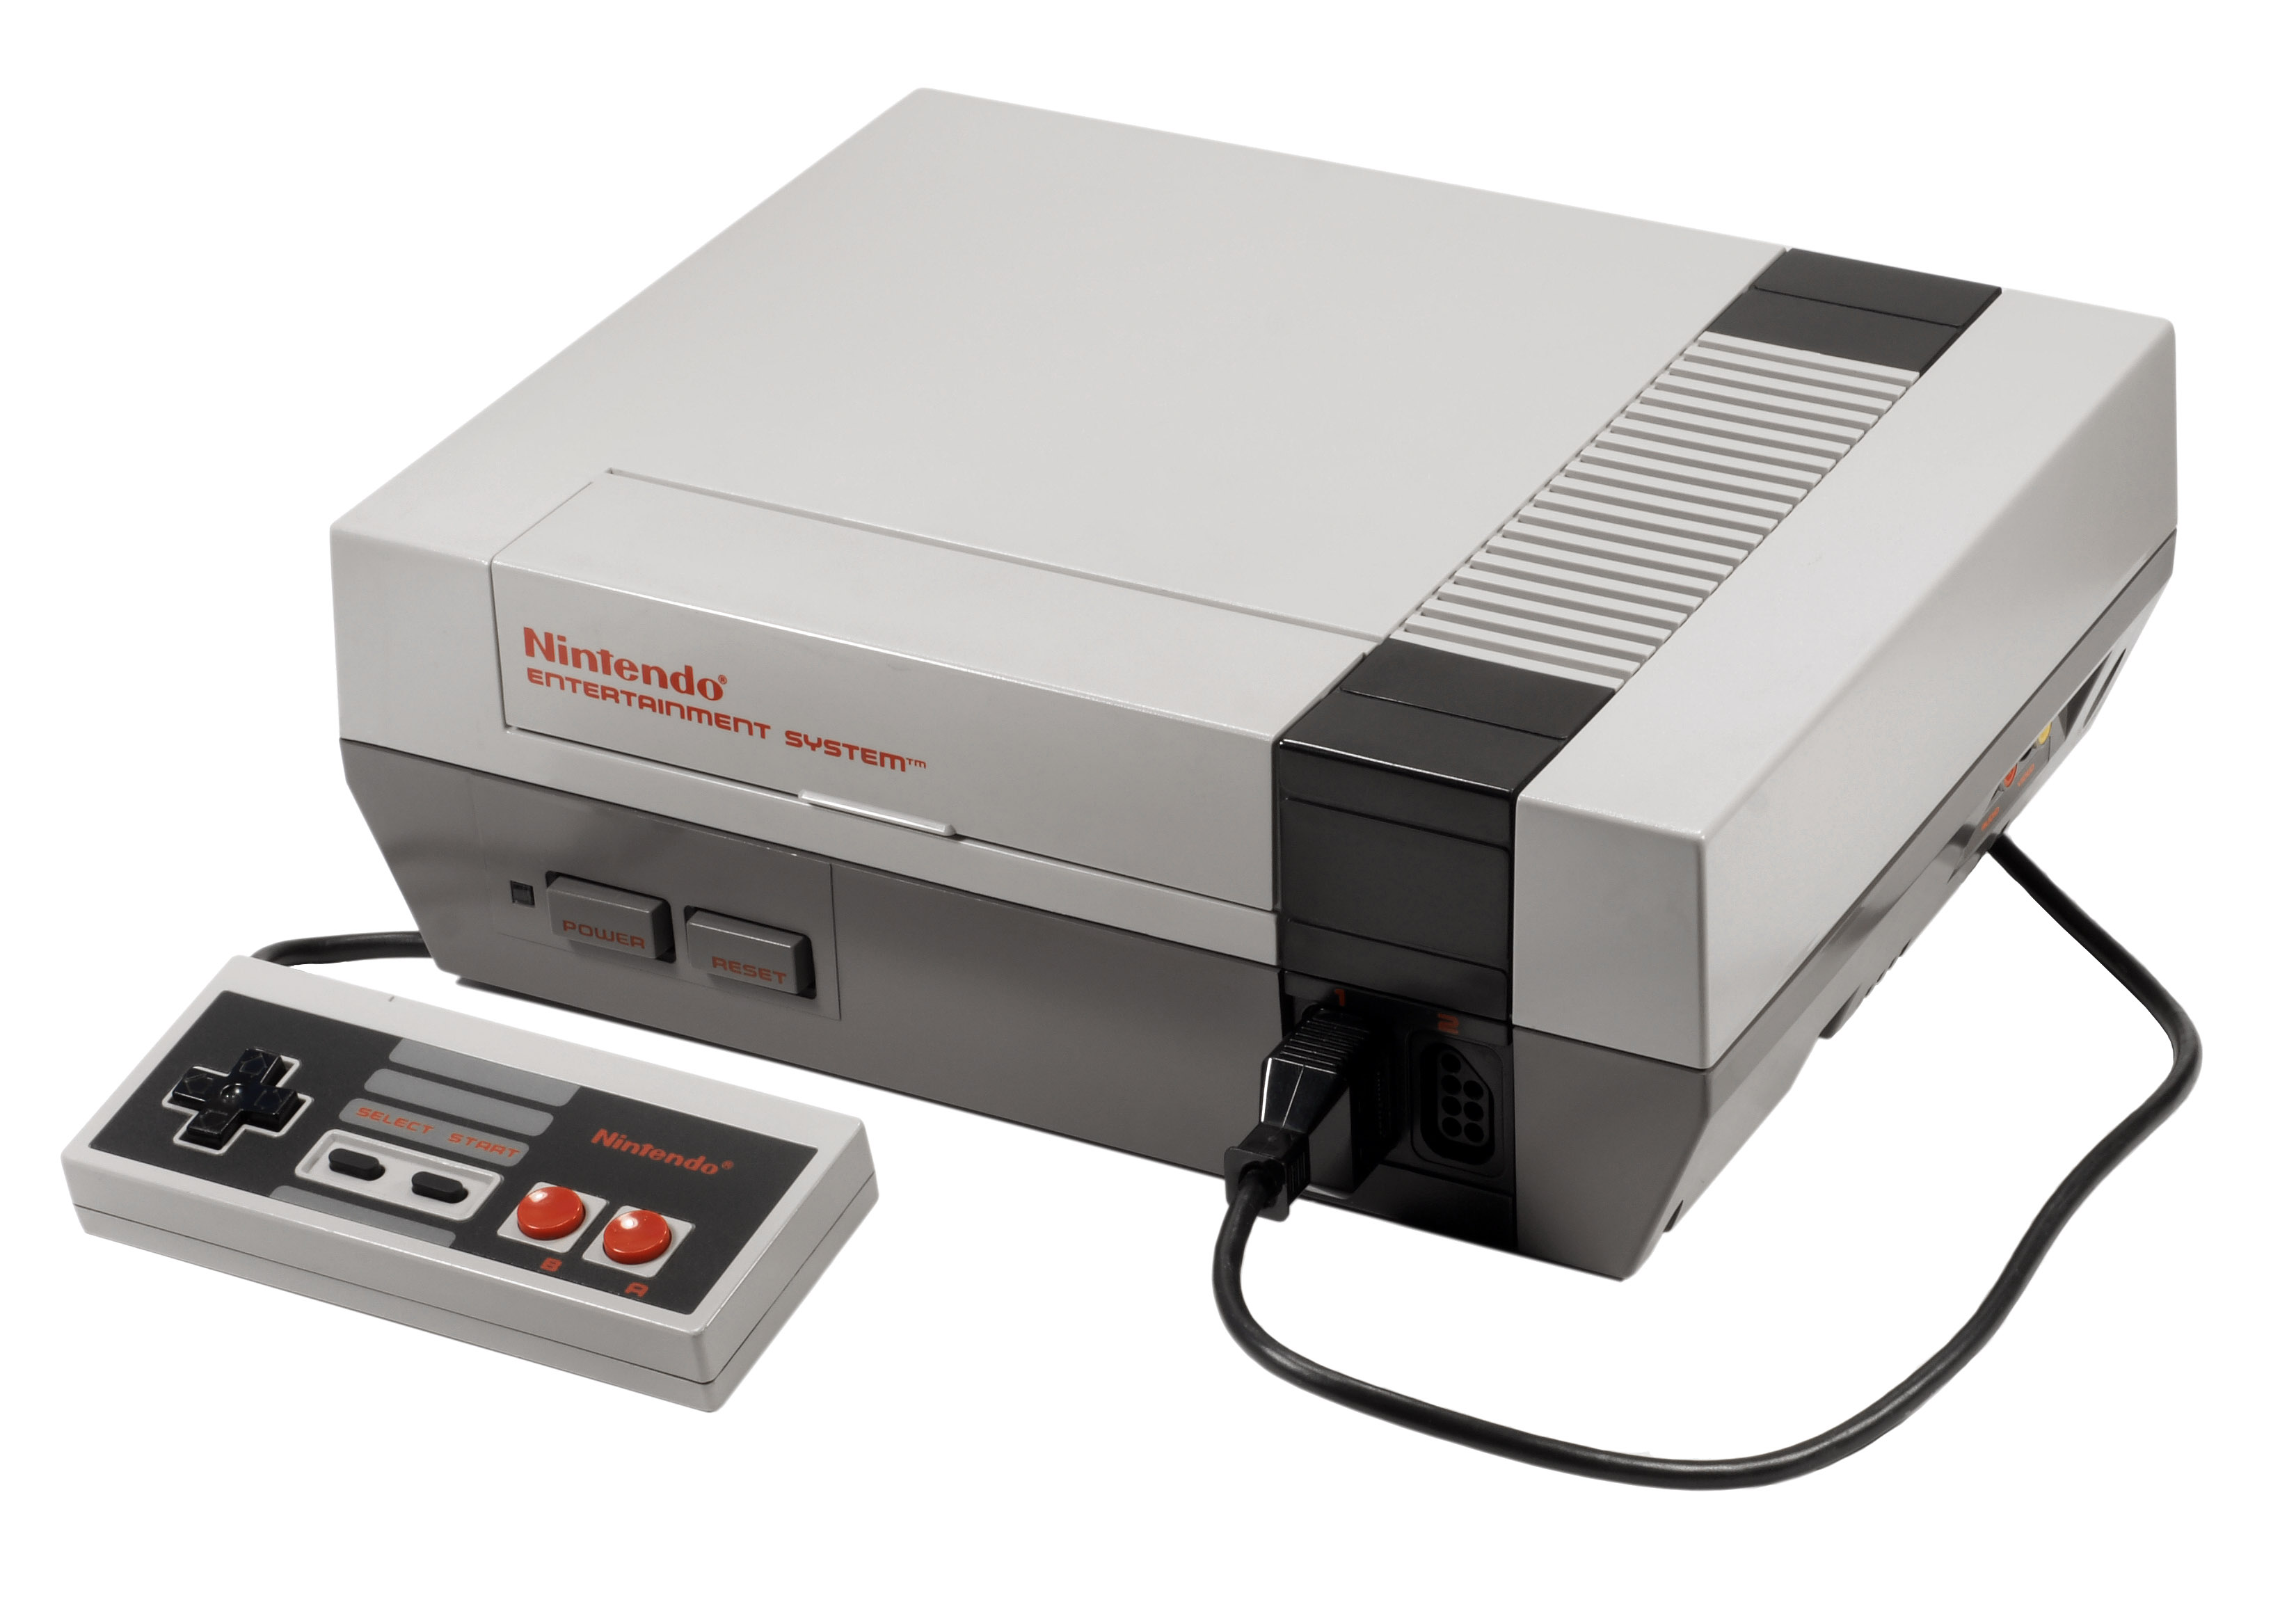
\includegraphics[width=120mm, keepaspectratio]{figures/NES-console-set}
	\caption{Nintendo Entertainment System}
	\label{fig:NES-Consol}
\end{figure}

Az otthoni konzol 8 bites processzorral rendelkezett, és a játékok tárolására elsősorban kazettákat használt. Jellegzetes, téglalap alakú kialakítása volt, a játékkazetták behelyezésére szolgáló elülső betöltő mechanizmussal. A konzolhoz egy pár kontroller is tartozott, és bevezette a ma már ikonikus NES gamepad kialakítását, amely irányjelzővel, start- és választógombokkal, valamint az A és B gombokkal rendelkezett.

A konzolra megjelent legnépszerűbb és legnagyobb hatású játékai közé tartozik a Super Mario Bros., a The Legend of Zelda, a Metroid, a Mega Man, a Castlevania és még sok más játék. Ezek a játékok megalapozták számos sikeres franchise-t, amelyek ma is virágoznak.

A játék konzol hardverének megismerésére, első sorban a hivatalos wiki oldalt használtam. Az itt olvasható tartalmakat az évek során nagy rész reverse engineering segítségével tárták fel, mivel a játék konzol pontos datasheet-jei, illetve időzítés és működési diagramjai nem lettek publikusak (a Nintendo tulajdonban vannak). Az itt szereplő adatokat a NESDev online közösség tartja karban, ezáltal az oldal pontos és helyes adatokat tartalmazhat (ezeket a közösség rendszeresen felül vizsgálja).   

\section{Képalkotás - Picture process unit}

A következőkben azt fogom bemutatni, hogy a NES hogyan tárol, dolgoz fel és jelenít meg sprite grafikákat. A Sprite egy 8x8-as pixel csempét jelent, ez a NES képalkotásának alap pillére.

A NES főkomponensei közül a Picture Process Unit (későbbiekben PPU) felelős a konzol 8-bit-es grafikájának elő állításáért. A PPU egy a Nintendo által kifejlesztett speciális chip amely a processzor mellett működik, mint egy társprocesszor (co-processor), hasonlóan a napjainkban elterjedt videó kártya processzor pároshoz.

A CPU-tól eltérően a PPU egy előre meghatározott grafikus műveleti parancs sorozatot hajt végre ciklikusan, nem lehet közvetlenül programozni. Saját memóriával rendelkezik
amelyet a CPU képes módosítani, hogy ezzel megváltoztassa a grafika generálását. Ez a memóriaterület a következőképpen négy részre oszlik:

\begin{itemize}
	\item \emph{Pattern táblák:} Az első szekció tartalmazza a pattern táblákat, amelyek a nyers sprite-kép adatokat tartalmazzák az adott játékhoz. Két pattern tábla van a bal oldali és a jobb oldali tábla amelyek mindegyike 64 kilobyte-nyi memória. Együttesen pedig 256 darab 8 x 8 pixeles csempét tárolnak. A memória ezen része általában közvetlenül 
	a játék kazetta karakter ROM vagy RAM chipjére van leképezve.
	\item \emph{Névtáblák (Nametables):} A következő rész a PPU névtábláit tartalmazza, amelyek a háttérgrafikák kialakítására szolgálnak a játékhoz. Ezek 32x30-as raszterben vannak felépítve, a raszter minden egyes eleme egy 8x8 pixeles területet reprezentál a képernyőn. A cellák egyetlen byte-ot tartalmaznak, amely egy csempét címez meg a Pattern táblákban.  
	\item \emph{Paletták (Palettes):} A harmadik rész az aktív szín paletták tárolására szolgál a játékhoz. A PPU képes több mint 50 különböző szín előállítására, de nem tudja az összes színt egyszerre használni egyidejűleg, ehelyett ezt a memória területet arra használják, hogy meghatározzunk nyolc aktív palettát amelyek egyenként négy színt tartalmaznak. Ebből a nyolc palettából, választhatunk színt a pixel-ek megjelenítése során.
	\item \emph{Objektum Attribútum Memória (későbbiekben OAM):} A PPU memóriának ez a része vezérli a játék előtérben lévő grafikáját megjelenítését, ezek olyan dolgok, mint például Mario, Link az ellenségek és az olyan effektek, mint a tűzgolyók és robbanások alapvetően bármi, ami a háttér grafika felett vagy néha alatta jelenne meg.
\end{itemize}

Tehát, mindezt összegezve, úgy tekinthetjük a PPU-ra, mintha ez a négy jól elkülöníthető memória terület irányítaná ezt a segéd processzort. A Pattern táblák határozzák meg a nyers kép adatok a névtáblák határozzák meg a háttér generálását, a paletták határozzák meg a használandó színeket és az OAM vezérli az előtérbe vagy háttérbe kerülő mozgó sprite-okat.
Ezen felül a PPU további funkciókkal is rendelkezik, ezeket nyolc különböző regiszter írásával és olvasásával érhetünk el. Ezekről a regiszterek az implementálása során \aref{sec:PPU-FPGA} fejezetben még olvashatunk.

	\subsection{PPU által generált kimeneti jel}
	\label{subsec:PPU-CRT}
	Ebben a fejezetben bemutatom a PPU által generált jelet és ennek felhasználást a régi típusú CRT TV-kben. A CRT televízió (az eredeti TV) a modern lapos képernyők előfutára volt, alapvetően két fő komponensből épültek fel egy fluoreszkáló képernyőből és egy katódsugárcsőből. 
	
	A CRT működése röviden: a katódsugárcső egy pisztolyként funkcionál, amely elektronokat lő ki a képernyőre és amikor elég elektron találja el a képernyő egy bizonyos területét az világítani kezd. A televíziók kétféle típusban léteztek fekete-fehérben vagy színesben. A fekete-fehér esetben egy elektronágyú szabályozta a képernyő pixel-einek monokróm fényerejét, a színes esetben három külön álló elektronágyú szabályozta a vörös, kék és zöld komponensek arányát, ezzel megalkotva a színes képet. A színes TV-k esetben is a három elektron sugár együtt mozgott végig a képernyőn, ezért a könnyebb megértés érdekében érdemes egy elektron sugárként gondolni ezekre. 
	
	A televízió működése során a bal felső sarokból kezdve úgy irányítja az elektron sugarat, hogy a teljes képernyőn végigfusson sorról sorra, amíg el nem éri a jobb alsó sarkát a képernyőnek. Ha egy sor végére érünk akkor az elektron sugarat vissza pozicionáljuk a sor elejére, ezt az időt horizontális szinkronizációnak nevezzük (horizontal balnking). Ha végig értünk egy kép kockán a TV a fegyvert újra a felső sor bal oldalára állítja, ezt vertikális szinkronizációnak (vertical blanking) hívják. Ez képalkotási ciklus a TV működése közben folytonosan ismétlődik rögzített időközönként általában másodpercenként hatvan képkocka körül. 
	
	%TODO ábra a CRT monitor képalktásáról
	\begin{figure}[H]
		\centering
		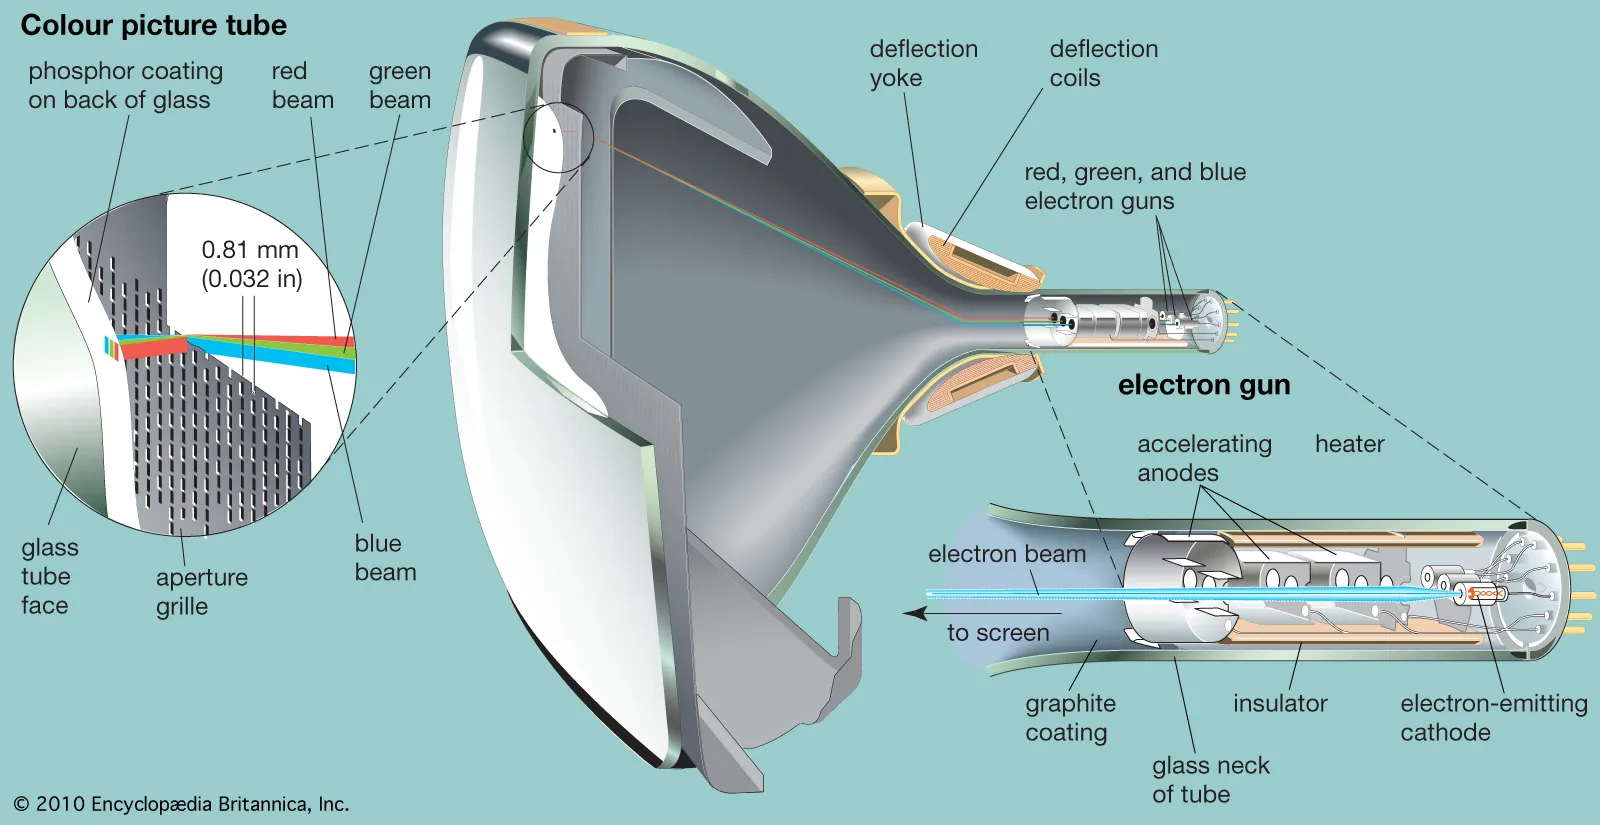
\includegraphics[width=150mm, keepaspectratio]{figures/CRT-TV}
		\caption{Katódsugárcsöves TV-k működése}
		\label{fig:CRT-TV}
	\end{figure}
	
	Miközben a elektronágyú mozog, a TV egy belső jel segítségével tudja szabályozni az elektronok kibocsátásának mértékét. Ez a jel megváltoztatja a szín fényerejét egy adott pozícióban (pixel-en), a pisztoly gyors mozgásának következtében, az eredmény egy folytonos animált kép képernyőn. Ezt a jelet kompozit jelnek nevezzük és általában egy rf antennáról vagy egy kábel boxból származott, de a NES esetében ezt a jelet a PPU állítja elő. 
	
	A NES két típusú kompozit jelet tudott elő állítani attól függően, hogy a világ melyik területére gyártották. Ez azért következett be mert a CRT TV-knek két standard típusa terjedt el világszerte az NTSC és a PAL. Az NTSC-t elsősorban az Egyesült Államokban és Japánban használták, és 60 képkocka/másodperces sebességgel jelenítette meg kompozit jelet, ezek a TV-k összesen 525 képsorral rendelkeztek. A PAL-t elsősorban Európában, Afrikában és Dél-Amerikában használták és 50 képkocka/másodperc sebességgel futott, összesen 625 képsort jelenített meg.
	
	A NES játékokat sosem programozták régió specifikusak, az egyetlen dolog ami változott területenként az a NES PPU-jának hardvere. Így a világ különböző területein ugyanaz a játék gyorsabban illetve lassabban futott, ez akár 17\%-os különbséget is jelenthetett. A NES emulálás szempontjából az NTSC készülékeket veszem alapul mivel ezeken gépek működését tárták fel részletesebben reverse engineering-el.
	
	\subsection{Pattern táblák és paletták}
	A sprite képek, amelyeket a PPU Pattern tábla memóriájában helyezkednek el, képezik az alapját minden grafikái megjelenítésnek. Ezek a  8 x 8 pixeles csempék alkotják a bonyolult háttereket, mozgó objektumokat és speciális effekteket. Alapvetően a sprite-ok tárolása hasonló módon történik mint egy modern számítógépek által használt kép esetében, mit például png. Mindkét tárolási formátumot kétdimenziós szám rácsként tudjuk elképzelni, ahol minden egyes cellához tartozó érték egy pixelhez tartozó színt reprezentál, csak amíg a png több millió színt támogat addig a NES egy pixel-e csupán négy különböző színű lehet. Gyakorlatilag egy ilyen csempe nem is tárol szín adatokat, a pixel-eket reprezentáló számértékek referenciák egy éppen aktív szín paletta színére.
	
	\begin{figure}[H]
		\centering
		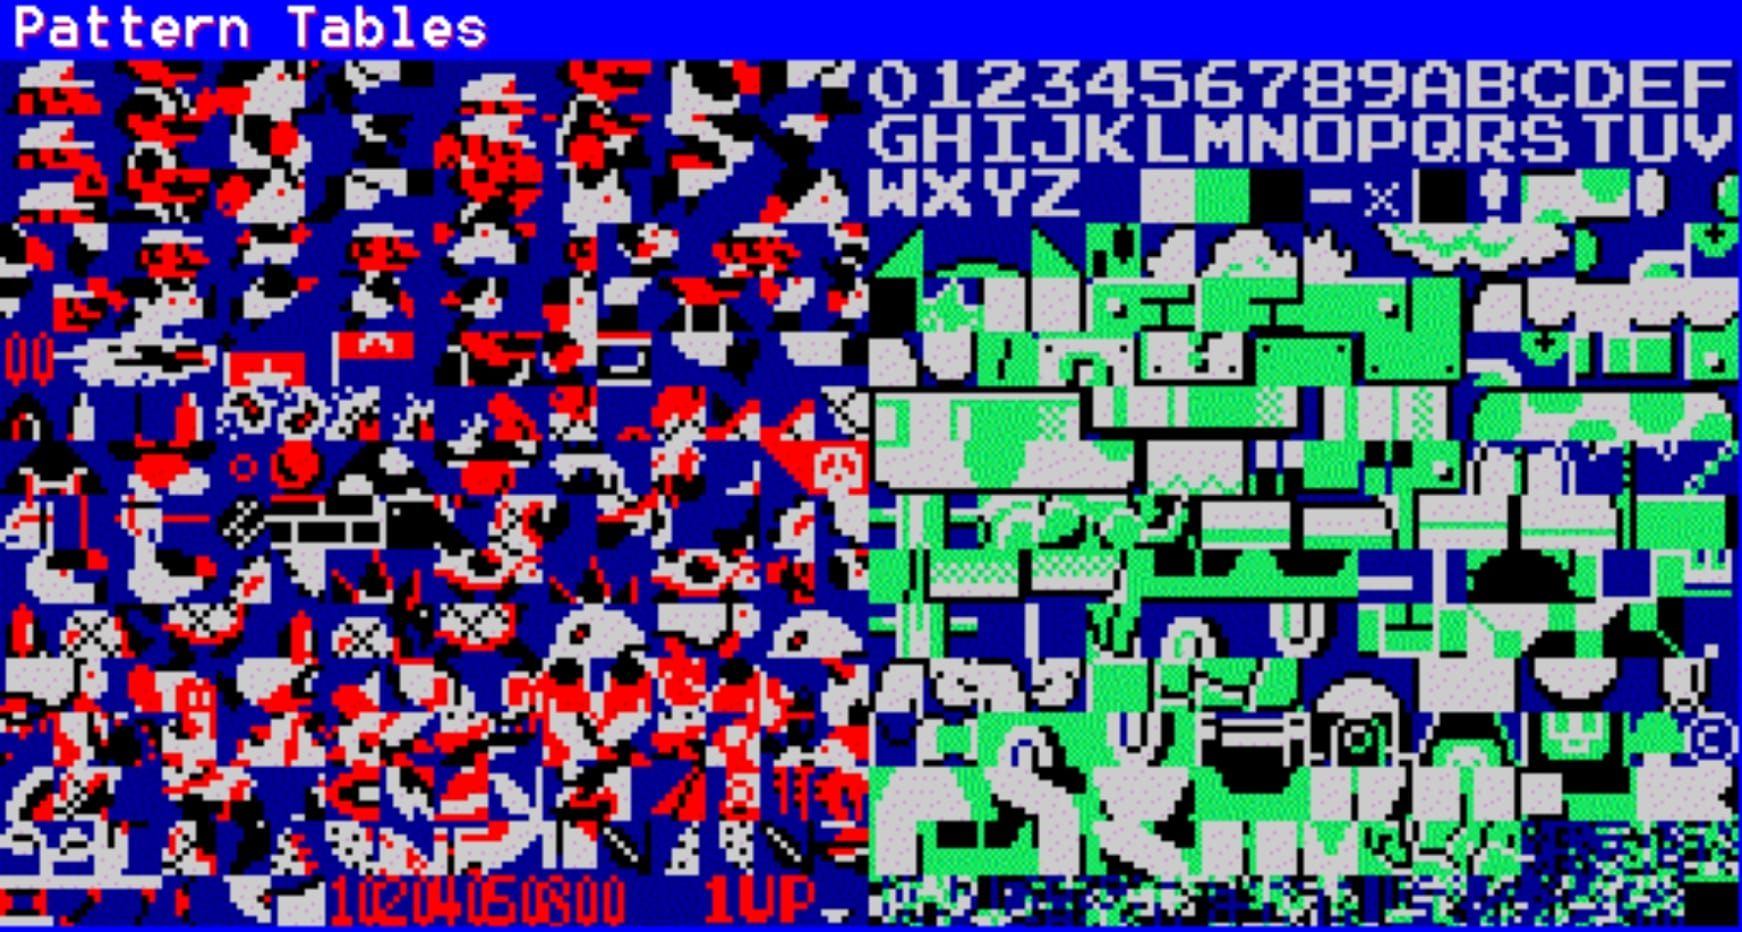
\includegraphics[width=150mm, keepaspectratio]{figures/Mario-Patterns}
		\caption{Super Mario Bros. Pattern táblái}
		\label{fig:Mario-Pattern}
	\end{figure}
	
	A szín paletták memória területének írásával, nyolc különböző palettát állíthatunk be a grafikus megjelenítéshez, négyet a háttér megjelenítéséhez és a maradék négyet az előtér rendereléséhez. Minden egyes paletta négy színt tárol, az első szín minden egyes palettán egy átlátszósági szín, ez azt jelenti, hogy ha a pixel szín értéke nullás indexel rendelkezik akkor az megjelenítés során minden esetben átlátszó lesz (függetlenül a palettába írt szín értéktől).
	
	A fentiek alapján, tehát egy pixel 0-3-ig vehet fel értéket, tehát 2 biten vagyunk képesek eltárolni az értékét. Egy 8 x 8 as csempe pedig 64 pixelt tartalmaz, ezért összesen 16 byte helyet foglal. Mivel a NES processzora egy 6502-es (8 bit-es) modell volt, ennek okán a legkisebb memória egység amit képes volt megcímezni az egy byte volt, így a csempe adatok ésszerű tárolásához egyedi megoldásra volt szükség.
	
	%todo ábra egy spriteról
	\begin{figure}[H]
		\centering
		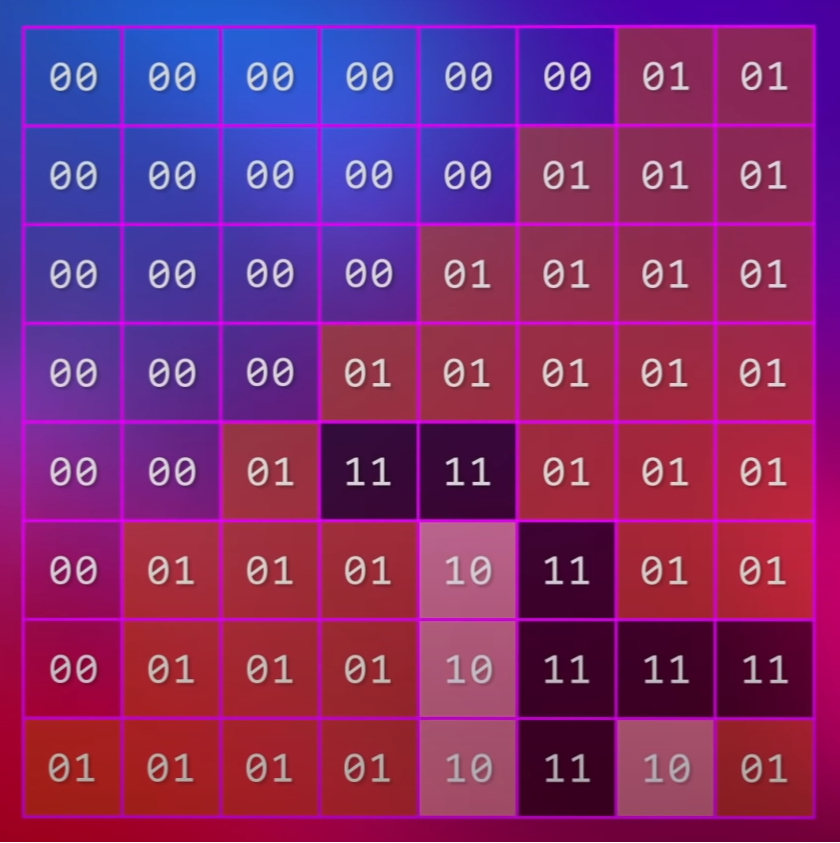
\includegraphics[width=100mm, keepaspectratio]{figures/Gumba-tile}
		\caption{Gumba (Mario egyik ellenfele) bal felső csempe elem szín adatai}
		\label{fig:Gumba-tile}
	\end{figure}

	Mivel a NES nem képes direkt a 2 bit-es számértékekkel dolgozni, ezért ezeket fel daraboljuk először logikailag magas és alacsony bitekre. Ezt követően elsőként a csempe alacsony 8 byte-ját tároljuk el majd ezt követően a magas nyolc byte-ot, így megkapjuk a fentebb kiszámolt 16 byte-os értéket. Ezáltal könnyel elérhetővé tettük a kép adatainkat a cpu számára, illetve a PPU-is helyesen képes ezeket megjeleníteni.
	
	\subsection{A név táblák és tulajdonság táblák (Attribute tables)}
	
	A név táblák alapvetően, ahogyan már fentebb olvashattuk egy-egy 32 x 30-as rácsként képzelhetők el, ahol minden egyes cella egy csempének felel meg (8 x 8 pixel). Ebből következően egy név tábla 256 x 240 pixelt tartalmaz, ez a CRT monitorok teljes képernyő területe. Egy rács elem, pedig egy, egy byte-os címet tartalmaz, amely az éppen aktív pattern tábla egy csempéjét címzi meg (mivel összesen 256 aktív csempénk lehet ezért elég egy byte a címzéshez).
	
	Ahhoz, hogy a PPU-nk képes legyen egy játék során gyors és gördülékeny háttér változásokra több különböző eszközt fejlesztettek ki. Kezdve azzal, hogy a NES hardveren belül két név táblát helyeztek el, ezek okos címzésével és a hardver sajátosságainak kihasználásával (mirroring) képesek vagyunk az úgy nevezett scrolling megvalósítására. Ez egyszerűen egy vertikális vagy egy horizontális finom lapozásnak írható le (egy-két sor pixel eltolásával, illetve megjelenítésével). Alapvető esetben a NES játékok vagy fix háttérrel rendelkeztek (lásd donkey kong), vagy csak horizontális vagy vertikális scrolling-ot alkalmaztak (horizontális - Super Mario Bros.). Viszont a későbbiekben megjelentek komplexebb játékok is amelyek ezek vegyítését alkalmazták ilyen például a Metroid vagy a Legend of Zelda.
	
	A mirroring az a jelenség, amikor két cím azonos memória területre mutat, ez azért fordulhat elő, mert a PPU nem teljes címzést használ (kevesebb bit-tel címez meg tartományokat). A név táblák esetében például egy 2 x 2-es rácsot szoktak képezni ennek segítségével, így kiterjesztve a két névtáblánk címzési tartományát. De ez a jelenség ez egész PPU memória felépítése során megfigyelhető.
	
	%todo memória map
	\begin{table}[H]
		\footnotesize
		\centering
		\begin{tabular}{|l|l|l|}
			\hline
			\rowcolor[HTML]{C0C0C0} 
			\multicolumn{1}{|c|}{\cellcolor[HTML]{C0C0C0}\textbf{Memórai címek}} & \multicolumn{1}{c|}{\cellcolor[HTML]{C0C0C0}\textbf{Méret}} & \multicolumn{1}{c|}{\cellcolor[HTML]{C0C0C0}\textbf{Leírás}} \\ \hline
			$0000 - $0FFF                                                        & \$1000                                                      & Pattern tábla 1                                              \\ \hline
			$1000 - $1FFF                                                        & \$1000                                                      & Pattern tábla 2                                              \\ \hline
			$2000 - $23FF                                                        & \$0400                                                      & Név tábla 1                                                  \\ \hline
			$2400 - $27FF                                                        & \$0400                                                      & Név tábla 2                                                  \\ \hline
			$2800 - $2BFF                                                        & \$0400                                                      & Név tábla 3                                                  \\ \hline
			$2C00 - $2FFF                                                        & \$0400                                                      & Név tábla 4                                                  \\ \hline
			$3000 - $3EFF                                                        & \$0F00                                                      & A $2000 - $2EFF címterület mirror-ja                         \\ \hline
			$3F00 - $3F1F                                                        & \$0020                                                      & Szín paletta RAM indexek                                     \\ \hline
			$3F20 - $3FFF                                                        & \$00E0                                                      & A $3F00 - $3F1F címterület mirror-ja                         \\ \hline
		\end{tabular}
		\caption{A PPU memória kezelése (14 bit címek) mirroring jelenséggel}
		\label{tab:PPU-memory}
	\end{table}
	
	Minden egyes névtábla végén egy kisebb extra memória terület található, amelyet tulajdonság táblának (vagyis Attribute Table-nek) nevezünk. Ez egy kisebb táblázatként képzelhető el ahol miden egyes cellában egy byte adatot tárolunk, viszont ennek feloldása bonyolultabb mint névtáblák esetében. Ez a 8 bit egy 4 X 4 csempényi háttér terület szín palettáját határozza meg a következő képen:
	
	\begin{itemize}
		\item az első két bit a bal felső 2 x 2 csempe palettáját határozza meg, 
		\item a második két bit a jobb felső 2 x 2-es terület palettáját határozza meg, 
		\item a harmadik két bit a bal alsó 2 x 2-es terület palettáját határozza meg,
		\item végül pedig az utolsó két bit a jobb alsó terület színérért felelős.
	\end{itemize}
	
	 Így a teljes képünket 8 x 8 ilyen byte al írhatjuk le. 
 
 	 \subsection{Objektum Attribútum Memória (OAM)}
 	 Ez a memória terület 64 külön álló sprite tárolására képes. Minden egyes OAM spritehoz négy byte adat tartozik. Az első byte meghatározza a vertikális vagy y koordinátáját a sprite-nak. A második byte azt határozza meg, hogy melyik 8 x 8-as csempe legyen megjelenítve az éppen aktív Pattern táblából. A harmadik byte segítségével különböző tulajdonságait vagyunk képesek befolyásolni a sprite-nak. Végül pedig az utolsó byte a horizontális vagyis x koordinátáját határozzam meg az objektumnak.
 	 
 	 Az előbb bemutatott byte-ok közül az egyetlen bonyolultabb működésű a harmadik, ebben az estben is a különböző bit-ek más és más működést kódolnak.  Az nulladik és az első bit egy előtér szín palettát választanak ki a sprite számára. A következő három bit (3, 4 és 5) nem használtak. Ezt követően az ötödik bit határozza meg, hogy a sprite a háttér elé vagy mögé kerüljön (ha értéke nulla akkor a háttér fölé fog kerülni, ha pedig egy mögé). Végül pedig a hatodik illetve hetedik bitek azt határozzák, hogy a sprite pixel-ei horizontálisan vagy vertikálisan helyet cseréljenek (tükrözve legyenek), nulla esetén a sprite eredeti formájában marad, egy esetén, pedig meg tükröződik. Ez egy nagyon hasznos tulajdonság, hiszen így a játék fejlesztők rengeteg memória területet spórolhattak a Pattern táblákból. Mivel több olyan objektumot, karaktert vagy effektet is tervezhettek amelyek vagy horizontálisan vagy vertikálisan szimmetrikusak voltak (erre az egyik legjobb példa a felvető gomba  a Super Mario Bros. videojátékból).    
 	     
 	 \subsection{PPU hardveres bug-ok}
 	 Mivel hardveres emulálást készítünk, ezért nem mehetünk el az eredeti hardver bug-jai mellett. Az esetek többségében a NES játék fejlesztői kihasználták ezeket az hazárdokat bug-okat a játékfejlesztéseik során. Tehát ha az eredeti játékokkal szeretnénk játszani ezekkel is maradéktalanul meg kell ismerkednünk.
 	 
 	 A PPU leghíresebb, ilyen bug-ja a Sprite Overflow Bug. Ez a OAM feldolgozása és megjelenítése közben alakulhat ki a NES-ben. Ennek megismeréséhez először is érdemes áttekinteni, hogy a PPU milyen állapot gép alapján dolgozza fel a OAM-ot. A PPU-n belül található egy másodlagos OAM amely nyolc sprite eltárolására képes, ennek a nyolc spritenak a megjelenítése történik a NES egy 256 pixeles sorban. Minden egyes sorral ebbe a memória területbe töltjük be az éppen aktív spritokat, ennek következtében a 64 sprite közül csupán nyolcat tudunk egy sorba megjeleníteni. Ezek alapján az OAM megjelenítés a következő négy lépésből áll:
 	  
 	 \begin{enumerate}
 	 	\item először is megtisztítjuk a másodlagos OAM-ot,
 	 	\item majd végig vizsgáljuk a teljes OAM-ot és kiválasztjuk azokat a sprite-okat amiket a következő sorban meg kell jeleníteni (ezekből az első nyolcat),
 	 	\item ha a megtaláltuk a 8 megjelenítendő sprite-ot akkor sajnos egy hibás implementációval végig vizsgálja az eszköz, hogy van-e még aktív sprite a sorban (ha talál ilyet beállítja a Sprite Overflow Flaget),
 	 	\item végül pedig a PPU feltölti a megjelenítéshez szükséges regisztereket az éppen aktív spritok adataival.
 	 \end{enumerate}
 	 
 	 A következő sorban megjelenítendő aktív sprite-ok kiválasztása, az objektumok y értéke alapján történik az OAM-ban tárolt prioritási sorrend alapján. A fent említett bug a harmadik lépésben következhet be, amikor a PPU megtalálta a nyolcadik sprite-ot ezt követően elkezdi vizsgálni a maradék OAM területet, viszont ennek vizsgálata csak az első esetben következik be helyes tulajdonság szerint (y érték). Ezt követően a a sprite-ok tulajdonságaiban diagonálisan haladunk (tehát a második keresés a Pattern tábla cím alapján történik, és későbbiekben így tovább halad az objektum négy byte-ján keresztül), így olyan esetben is bejelezhet a Sprite Overflow Flag amikor ez nem is történt meg. Erre a bug-ra több híres játék is épített az egyik leghíresebb a The Legend of Zelda, de például a Ninja Gaiden és Castlevania sorozatokban is meg jelent.
 	 
 	 Egy másik kevésbé ismert bug-ot az OAMADDR regiszterrel kapcsolatban találtak meg. Ez általában akkor jött elő amikor nem a DMA vezérlőt használták az OAM frissítésére, hanem a szimpla byte elérését. Ilyenkor néha elő fordult, hogy egy egy byteot rossz OAM területre másolt az eszköz, ezzel beszennyezve az OAM-ot. Ennek a bug-nak későbbi kompatibilitási okai voltak.    
 	 
 	       
\section{2A03 a NES CPU-ja}

A fent szereplő 2A03 egy elterjedt rövidítés a RP2A03[G] típusú 8 bites CPU-ra, amely a NTSC típusú NES CPU egysége. Ez a  

	\subsection{6502 - Central processing unit}

	\subsection{Audio process unit}

\section{Belső memória}

\section{játék kártyák - mapperek}
\chapter{NES FPGA alapú újra gondolása}

\section{Képalkotás}

\section{Audio}

\section{Játékok tárolása}

\section{Kompakt hordozható méret}



\chapter{FPGA NES kártya ismertetése}

A NES hardverének újragondolásából \aref{fig:PCB-blockdiagram} ábrán látható blokk diagramot készítettem, ez a nyomtatott huzalozott kártyák tervezésének első lépése. Már itt érdemes feltüntetni a különböző áramköri elemek közti kommunikációs utakat (busz típusokat), illetve ezek irányát. Ez alapján a diagram alapján, pedig elkezdődhet a különböző komponensek keresése, ezt követően át kell gondolnunk ezek fogyasztását és feszültség szintjeit ezekből az adatokból pedig megtervezhető a kártya táp ellátása is (a mi esetünkben már kiegészítettem ezzel a blokk diagramot). 

\begin{figure}[H]
	\centering
	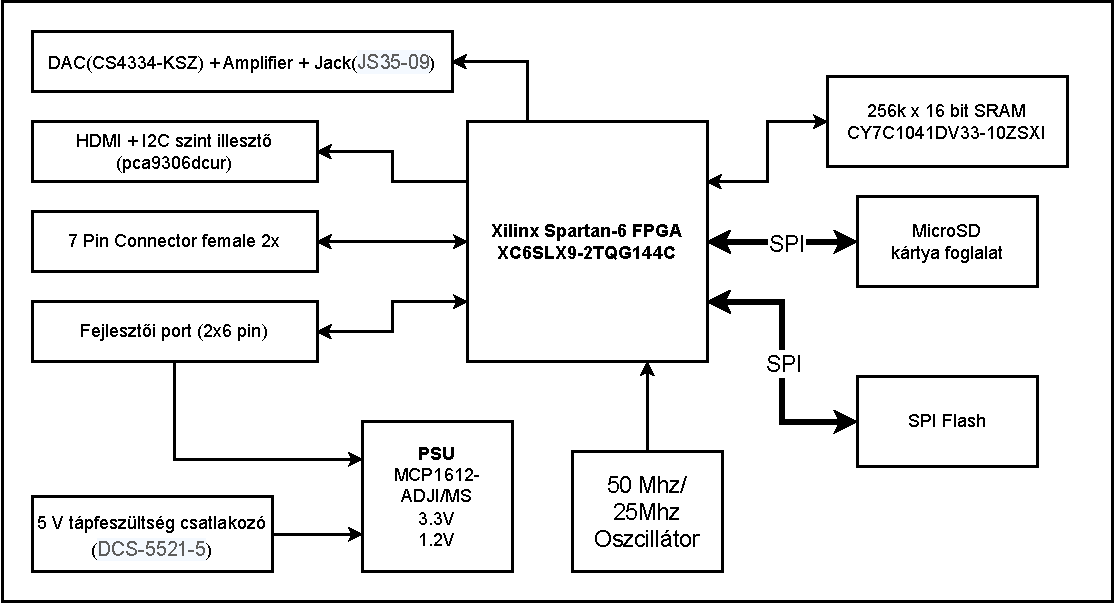
\includegraphics[width=150mm, keepaspectratio]{figures/NES-board-blockdiagram}
	\caption{NES kártya blokkdiagramja}
	\label{fig:PCB-blockdiagram}
\end{figure}

A komponensek, közül az FPGA chip kiválasztása a legnehezebb, ennek menete általában az, hogy megpróbáljuk felmérni a hardverünk méretét és ez alapján választunk megfelelő méretű chip-et. A mi esetünkben az egyik legkomplexebb elem a 6502-es 8-bites processzor amely méretét az OpenCores weboldalon található nyílt forráskódú hardver tervek alapján megbecsülhetjük körülbelül 1000 LUT-ra. Mivel NES hardver működéséhez három fő komponens kell (CPU, APU, PPU) ezek méretét egyesével felülbecsülhetjük a legkomplexebb alkatrész méretével, így összesen 3000 LUT-ot kapunk. Ehhez még érdemes a VGA jel elő állítását (HDMI jel kódolása), illetve az audió jel kezelését még hozzá számolni, erre is jó felső becslés az 1000 LUT. Végül még érdemes tartalékkal is számolni ezért egy 5000-6000 LUT-al rendelkező FPGA chip valószínűleg elég nagy ahhoz, hogy a teljes projekt elférjen benne. Fontos kritérium még, hogy DCM-el illetve PLL-el rendelkezzen a chip az egyedi órajelek előállítása érdekében (például a 250 MHz a VGA bit-ek kiadásához), ezen kívül még Blokk-RAM-ra is szükség lesz legalább akkorára mint a NES hardverének belső memóriája (például Név táblák 2 kilobájt).  

%todo kell e ide a konzulens hivatkozása Szerencsére a konzulensem jóvoltából, szert tettem
A feladat megvalósításához egy Spartan-6-os Xilinx FPGA állt a rendelkezésemre, amely megfelel a fent említett összes elvárásnak. Ez a chip nagyban meggyorsította a nyáktervezés menetét is, mivel az egyetemi Spartan-6-os fejlesztő kártyák fő komponense is ez az FPGA volt (erről itt olvashatunk részletesebben \cite{spatan6}). Ezt a fejlesztő kártyát vettem alapul a NES kártyám fejlesztő portjának kialakítása, az SPI flash bekötése, illetve a táp vonalak kialakítása során is. 
	
A kártyán az alábbi komponensek találhatók:

\begin{itemize}
	\item \emph{FPGA:} Xilinx XC6SLX9-2TQG144C típusú Spartan-6-os FPGA, amely lehetővé teszi összetettebb logikák és
	mikroprocesszoros rendszerek megvalósítását. Az eszköz főbb jellemzői:
		\begin{itemize}
			\item 5720 darab 6 bemenetű LUT és 11440 darab flip-flop
			\item 32 darab 18 kilobites blokk-RAM
			\item 16 darab DSP48A1 blokk (elő összeadó, 18 x 18 bites előjeles szorzó és akkumulátor)
			\item 4 darab DCM (Digital Clock Manager) és 2 darab PLL (Phase Locked Loop) modul
		\end{itemize} 
	\item \emph{Memóriák a program és az adatok tárolására:}
		\begin{itemize}
			\item Egy 256k x 16 bites (512 kB), 10 ns-os aszinkron SRAM (Cypress CY7C1041DV33-10ZSXI)
			\item Egy 32 Megabites SPI buszos soros FLASH memória (Atmel AT25DF321A), amely
			konfigurációs memóriaként is szolgál az FPGA számára
		\end{itemize}
	\item \emph{Egy MicroSD memóriakártya foglalat:}
		\begin{itemize}
			\item Teljes MicroSD kártya protokoll
			\item Egyszerű SPI protokoll
		\end{itemize}
	\item \emph{Beviteli eszközök:}
		\begin{itemize}
			\item Két eredeti 7 lábas NES (GamePAD) kontroller csatlakozók
			\item Reset és PROG gombok
		\end{itemize}	
	\item \emph{Képfeldolgozás:}
		\begin{itemize}
			\item HDMI csatlakozó 
			\item I2C szint illesztő (PCA9306DCUR típusú), a HDMI audió vonalainak illesztéséhez 
		\end{itemize}
	\item \emph{Audio:}
		\begin{itemize}
			\item Digitális-analóg átalakító (DAC), CS4334-KSZ típusú  
			\item 100mW Erősítő TS486IST típus (fülhallgatókhoz)
			\item CUI SJ1-3553NG 3.5mm Jack csatlakozó
		\end{itemize}
	\item \emph{Tápegységek:} MCP1612-ADJI/MS típusú szinkron Buck konverterek
	\item \emph{Egy 50 MHz-es oszcillátor} 
	\item \emph{Csatlakozó a LOGSYS fejlesztői kábel számára} 
\end{itemize}
	
\section{Tápellátás}
	
	A tápellátás kialakítása a Logsys Spartan-6-os fejlesztői kártyáéhoz hasonló \cite{spatan6}. A NES kártya 5 V-os tápfeszültségről működik. Ezt a tápellátást, vagy a fejlesztő kábelről kapja az eszköz, vagy egy külső 5 V-os forrásból. A külső egyenfeszültségű forrás Shottky diódával védtem, illetve a kártyát töltést jelző zöld led-del is elláttam (PWR). 
	
	Az 5 V-os forrást két azonos típusú step down (Buck) konverterrel 3.3 V-ra és 1.2 V-ra konvertálom. Alapvetően az FPGA működéséhez kell a két feszültség szint. A 3.3 V az I/O vonalakért, DCM, PLL, és konfigurációért felelős, az 1.2 V pedig az FPGA belső magjának kell. Ezt a két tápvonalat az FPGA dokumentációja alapján (a táp lábaihoz közel) elláttam a megfelelő mennyiségű csatoló (coupling) és hidegítő (bulk) kapacitásokkal a stabil működés végett. A 3.3 V-ot a kártyán található többi alkatrész is használja (SRAM, MicroSDkártya, kontrollerek, a fejlesztő kábel is megkapja mint JTAG referencia feszültség ként stb.). Illetve a kártya a HDMI csatlakozó, DAC és erősítő komponensek esetén, a tápellátás 5 V-ját is felhasználja. A tápellátás schematik rajzát \aref{sec:PSU} függelékben láthatjuk. 
	 
\section{Órajel források}
	
	A NES kártyán a Logsys fejlesztő kártyához hasonlóan, egy 50 MHz-es oszcillátort helyeztem el. Az FPGA, vagy a fejlesztő portról érkező CLK-től kapja az órajelét, vagy ezt az 50 MHz-es CLK-t használja. Ahhoz, hogy az FPGA használhassa ezeket az órajeleket egy-egy órajel bemeneti lábára (GCLK) kellet ezeket bekötni. Az oszcillátor segéd áramkörét \aref{sec:OSC-JTAG} függelékben láthatjuk. % és órajel források bekötését pedig \aref{tab:FPGA-OSCpin} táblázatban olvashatjuk.
	
%	\begin{table}[H]
%		\footnotesize
%		\centering
%		\begin{tabular}{|l|l|}
%			\hline
%			\rowcolor[HTML]{C0C0C0} 
%			\multicolumn{1}{|c|}{\cellcolor[HTML]{C0C0C0}{\color[HTML]{333333} \textbf{Órajel forrás}}} & \multicolumn{1}{c|}{\cellcolor[HTML]{C0C0C0}{\color[HTML]{333333} \textbf{FPGA láb}}} \\ \hline
%			50 MHz-es oszcillátor                                                                       & P85                                                                                   \\ \hline
%			Fejlesztői port CLK vonala                                                                  & P95                                                                                   \\ \hline
%		\end{tabular}
%		\caption{FPGA órajel forrásainak bekötése}
%		\label{tab:FPGA-OSCpin}
%	\end{table}
	
\section{Memória - SRAM}
	
	A választott asszinkron SRAM mérete 256 k x 16 bit (byte-okban mérve 512 k), ez a méret megfelel \aref{sec:Game-store} fejezetben tárgyalt játék méreteknek (csak egy NES játék nem fog beleférni ebbe a RAM-ba). A választott memória előnye, hogy 10 ns elérési idejű asszinkron, statikus RAM, egyszerű kezeléssel. Ez azért jelent előnyt a konzol hardveres emulálása szempontjából, mert nem fogja ennek működését befolyásolni a memória elérési idő (a későbbiekben az elérést igazíthatjuk az általunk választott időzítéshez). DRAM esetén sokkal több időzítési paraméterrel kell számolni ez természetesen jóval megnehezíti a időzítés kritikus hardver létrehozását.
	
	Az SRAM 18 bites címmel rendelkezik, amellyel megcímezhetők a 2 byte-osával az adataink (256 k cím). A RAM-ból kiolvasott, illetve beírandó adatokat pedig a 16 bit-es adat vonalak olvasásával és írásával érhetjük el. Az SRAM vezérlésétől függően kiolvasható vagy írható egyszerre mind a 16 bit, de van byte-os elérési mód is.
	
	Az SRAM szabványos vezérlési felülettel rendelkezik. Tehát következő vezérlő jelek segítségével tudjuk irányítani (ezek mindegyike negált logikájú): chip engedélyezés CSn, írás engedélyezése WEn, olvasás engedélyezés OEn, alsó byte engedélyezés LBn, végül pedig a felső byte engedélyezés UBn. A memória olvasási és írási idő diagramjait \acite{sram} adatlapon olvashatjuk, kiegészítő áramkörét pedig \aref{sec:SRAM-SPI-Flash} függelékben láthatjuk.     
	
%	\begin{table}[H]
%		\footnotesize
%		\centering
%		\begin{tabular}{|lccccccccc|}
%			\hline
%			\rowcolor[HTML]{C0C0C0} 
%			\multicolumn{10}{|l|}{\cellcolor[HTML]{C0C0C0}\textbf{Címbusz}}                                                                                                                                                                                                                                                                                                                                                                                                                                                                                                                                                                                                                                      \\ \hline
%			\rowcolor[HTML]{EFEFEF} 
%			\multicolumn{1}{|l|}{\cellcolor[HTML]{EFEFEF}SRAM}                            & \multicolumn{1}{c|}{\cellcolor[HTML]{EFEFEF}A0}                         & \multicolumn{1}{c|}{\cellcolor[HTML]{EFEFEF}A1}                         & \multicolumn{1}{c|}{\cellcolor[HTML]{EFEFEF}A2}                         & \multicolumn{1}{c|}{\cellcolor[HTML]{EFEFEF}A3}                         & \multicolumn{1}{c|}{\cellcolor[HTML]{EFEFEF}A4}                         & \multicolumn{1}{c|}{\cellcolor[HTML]{EFEFEF}A5}                         & \multicolumn{1}{c|}{\cellcolor[HTML]{EFEFEF}A6}                         & \multicolumn{1}{c|}{\cellcolor[HTML]{EFEFEF}A7}                         & A8   \\ \hline
%			\rowcolor[HTML]{EFEFEF} 
%			\multicolumn{1}{|l|}{\cellcolor[HTML]{EFEFEF}{\color[HTML]{333333} FPGA láb}} & \multicolumn{1}{c|}{\cellcolor[HTML]{EFEFEF}{\color[HTML]{333333} P47}} & \multicolumn{1}{c|}{\cellcolor[HTML]{EFEFEF}{\color[HTML]{333333} P46}} & \multicolumn{1}{c|}{\cellcolor[HTML]{EFEFEF}{\color[HTML]{333333} P45}} & \multicolumn{1}{c|}{\cellcolor[HTML]{EFEFEF}{\color[HTML]{333333} P44}} & \multicolumn{1}{c|}{\cellcolor[HTML]{EFEFEF}{\color[HTML]{333333} P43}} & \multicolumn{1}{c|}{\cellcolor[HTML]{EFEFEF}{\color[HTML]{333333} P34}} & \multicolumn{1}{c|}{\cellcolor[HTML]{EFEFEF}{\color[HTML]{333333} P33}} & \multicolumn{1}{c|}{\cellcolor[HTML]{EFEFEF}{\color[HTML]{333333} P32}} & P30  \\ \hline
%			\multicolumn{1}{|l|}{SRAM}                                                    & \multicolumn{1}{c|}{A9}                                                 & \multicolumn{1}{c|}{A10}                                                & \multicolumn{1}{c|}{A11}                                                & \multicolumn{1}{c|}{A12}                                                & \multicolumn{1}{c|}{A13}                                                & \multicolumn{1}{c|}{A14}                                                & \multicolumn{1}{c|}{A15}                                                & \multicolumn{1}{c|}{A16}                                                & A17  \\ \hline
%			\multicolumn{1}{|l|}{FPGA láb}                                                & \multicolumn{1}{c|}{P29}                                                & \multicolumn{1}{c|}{P7}                                                 & \multicolumn{1}{c|}{P6}                                                 & \multicolumn{1}{c|}{P5}                                                 & \multicolumn{1}{c|}{P2}                                                 & \multicolumn{1}{c|}{P1}                                                 & \multicolumn{1}{c|}{P139}                                               & \multicolumn{1}{c|}{P138}                                               & P137 \\ \hline
%		\end{tabular}
%		\caption{SRAM memória címbusz bekötése}
%		\label{tab:FPGA-MEM-SRAMpin}
%	\end{table}
%		
%	\begin{table}[H]
%		\footnotesize
%		\centering
%		\begin{tabular}{|lcccccccc|}
%			\hline
%			\rowcolor[HTML]{C0C0C0} 
%			\multicolumn{9}{|l|}{\cellcolor[HTML]{C0C0C0}\textbf{Adatbusz}}                                                                                                                                                                                                                                                                                                                                                                                                                                                                                                                                                                                  \\ \hline
%			\rowcolor[HTML]{EFEFEF} 
%			\multicolumn{1}{|l|}{\cellcolor[HTML]{EFEFEF}SRAM}                            & \multicolumn{1}{c|}{\cellcolor[HTML]{EFEFEF}D0}                         & \multicolumn{1}{c|}{\cellcolor[HTML]{EFEFEF}D1}                         & \multicolumn{1}{c|}{\cellcolor[HTML]{EFEFEF}D2}                         & \multicolumn{1}{c|}{\cellcolor[HTML]{EFEFEF}D3}                         & \multicolumn{1}{c|}{\cellcolor[HTML]{EFEFEF}D4}                         & \multicolumn{1}{c|}{\cellcolor[HTML]{EFEFEF}D5}                         & \multicolumn{1}{c|}{\cellcolor[HTML]{EFEFEF}D6}                         & D7                         \\ \hline
%			\rowcolor[HTML]{EFEFEF} 
%			\multicolumn{1}{|l|}{\cellcolor[HTML]{EFEFEF}{\color[HTML]{333333} FPGA láb}} & \multicolumn{1}{c|}{\cellcolor[HTML]{EFEFEF}{\color[HTML]{333333} P40}} & \multicolumn{1}{c|}{\cellcolor[HTML]{EFEFEF}{\color[HTML]{333333} P17}} & \multicolumn{1}{c|}{\cellcolor[HTML]{EFEFEF}{\color[HTML]{333333} P21}} & \multicolumn{1}{c|}{\cellcolor[HTML]{EFEFEF}{\color[HTML]{333333} P22}} & \multicolumn{1}{c|}{\cellcolor[HTML]{EFEFEF}{\color[HTML]{333333} P23}} & \multicolumn{1}{c|}{\cellcolor[HTML]{EFEFEF}{\color[HTML]{333333} P24}} & \multicolumn{1}{c|}{\cellcolor[HTML]{EFEFEF}{\color[HTML]{333333} P26}} & {\color[HTML]{333333} P27} \\ \hline
%			\multicolumn{1}{|l|}{SRAM}                                                    & \multicolumn{1}{c|}{D8}                                                 & \multicolumn{1}{c|}{D9}                                                 & \multicolumn{1}{c|}{D10}                                                & \multicolumn{1}{c|}{D11}                                                & \multicolumn{1}{c|}{D12}                                                & \multicolumn{1}{c|}{D13}                                                & \multicolumn{1}{c|}{D14}                                                & D15                        \\ \hline
%			\multicolumn{1}{|l|}{FPGA láb}                                                & \multicolumn{1}{c|}{P8}                                                 & \multicolumn{1}{c|}{P9}                                                 & \multicolumn{1}{c|}{P10}                                                & \multicolumn{1}{c|}{P11}                                                & \multicolumn{1}{c|}{P12}                                                & \multicolumn{1}{c|}{P14}                                                & \multicolumn{1}{c|}{P15}                                                & P16                        \\ \hline
%		\end{tabular}
%		\caption{SRAM memória adatbusz bekötése}
%		\label{tab:FPGA-DATA-SRAMpin}
%	\end{table}
%
%	\begin{table}[H]
%		\footnotesize
%		\centering
%		\begin{tabular}{|llllcc|}
%			\hline
%			\multicolumn{6}{|l|}{\cellcolor[HTML]{C0C0C0}\textbf{Vezérlő jelek}}                                                                                \\ \hline
%			\multicolumn{1}{|l|}{SRAM}     & \multicolumn{1}{l|}{CSn} & \multicolumn{1}{l|}{WEn} & \multicolumn{1}{l|}{OEn}  & \multicolumn{1}{c|}{LBn}  & UBn  \\ \hline
%			\multicolumn{1}{|l|}{FPGA láb} & \multicolumn{1}{l|}{P41} & \multicolumn{1}{l|}{P35} & \multicolumn{1}{l|}{P140} & \multicolumn{1}{c|}{P142} & P141 \\ \hline
%		\end{tabular}
%		\caption{SRAM memória vezérlő jelek bekötése}
%		\label{tab:FPGA-CONTROL-SRAMpin}
%	\end{table} 
	
\section{Digital Analog Converter és erősítő}
	
	A NES kártya egyetlen analóg alkatrészekre támaszkodó része a DAC-ot követő erősítő áramkör, ennek részletes megértéséhez tekintsük meg \aref{fig:DAC-AMP-JACK} ábrát, amely \aref{sec:DAC-controllers} függelékből lett kiemelve.
	
	A DAC komponenst egy 100MHz-en 600 $\Omega$-as Ferrite Bead-el védem, az esetleges 5 V-os tápvonalról beszűrődő zajokkal szemben, ide szűrési okokból tantál és kerámia kondenzátorokat is helyeztem. Az alkatrész az FPGA által elő állított mono digitális "hang" jelet, átalakítja és kiadja mind a két kimenetén. Ezek az analóg jelek fognak az erősítést követően, a Jack csatlakozó bal és jobb fülhöz menő lábára csatlakozni. 
	
	A DAC két kimenetét, egy egy 3.3 uF-os csatoló kondenzátorral választom el az analóg résztől. Az áramkörben található C38, C39-es kondenzátorok és R27, R28-as ellenállások egy alul áteresztő szűrőt valósítanak meg. A kondenzátorok értékét, pedig a következő képlet alapján határoztam meg (az ellenállások értéke kötött volt az erősítő miatt):
	
	\begin{align}	
		C = \frac{R + 560 \Omega}{4} *\pi * Fs * (R * 560 \Omega)
	\end{align} 
	
	Itt $Fs$ az általunk választott audió jel frekvenciája az 560 $\Omega$ pedig a soros ellenállás értéke. Ezek alapján a két kondenzátorom értéke 3.3 nF vagy 2.7 nF lehet, mivel így 48 KHz-hez közeli értéket kapunk a frekvenciára. Az összes kerámia kondenzátornak, amely az analóg áramkör része NP0 (vagy C0G) dielektrikummal kell rendelkeznie, mivel ezeknek nincs piezoelektromos tulajdonságuk.   
	
	\begin{figure}[H]
		\centering
		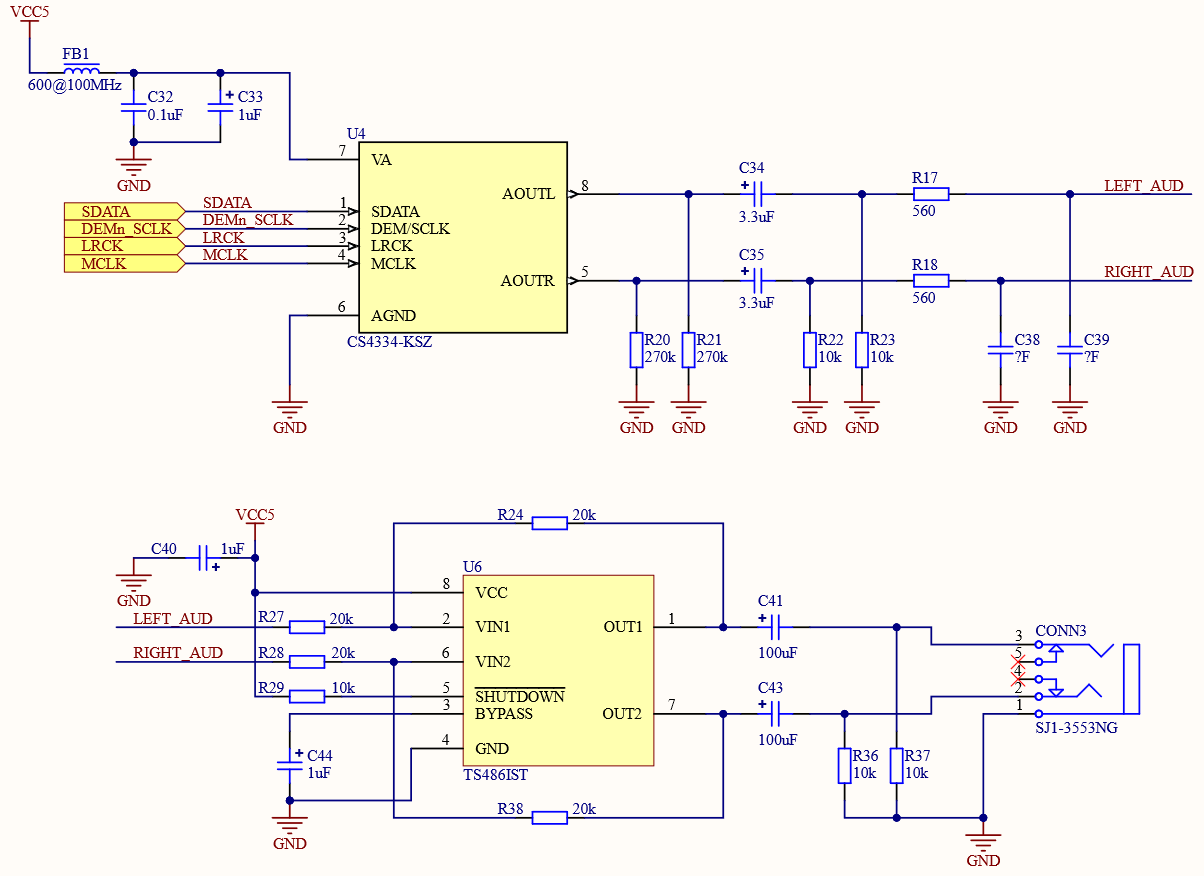
\includegraphics[width=150mm, keepaspectratio]{figures/DAC-AMP-JACK}
		\caption{NES audió jelért felelős áramkörök}
		\label{fig:DAC-AMP-JACK}
	\end{figure}
	
	Az erősítő komponensnek egy fázis fordító erősítőt választottam, amely erősítése az R24 és R38 ellenállásokkal módosítható a következő képletek alapján:
	
	\begin{align}	
		Gain_{LINEAR} = -\frac{RFEED}{RIN}
	\end{align} 
	
	\begin{align}	
		Gain_{dB} = 20 * lg(\frac{RFEED}{RIN})
	\end{align}
 
	Az áramkörben jelenleg nem állítottam be erősítést az RFEED és RIN ellenállások értékét 20 k$\Omega$-nak határoztam meg. Ez természetesen a hardveres tesztelés során cserélhető és állítható.	
	
\section{HDMI és I2C szint illesztő}
	\label{sec:HMI-I2C}
	
	A NES nyomtatott huzalozott kártyáján elhelyeztem egy HDMI csatlakozót és a körülötte elhelyezkedő áramkör segítségével felkészítettem VGA jelek kiadására. A teljes áramkör sematikus ábráját (schematic) \aref{sec:HDMI-MicroSDcard} függelékben láthatjuk.
	
	A jövőbeli fejlesztések miatt elhelyeztem a nyákon még egy I2C jel szint illesztőt is, amely segítségével az FPGA 3.3 V-on működő lábait, a HDMI audió jel kiadásáért felelős lábaihoz (SCL/SDA) illesztem. Így a kártya támogatja a TV-k és monitorok beépített hangszóróit is. 
	
	Az alábbi ábrákon láthatjuk és olvashatjuk egy HDMI anya aljzat pin és láb kiosztását:   
	
	\begin{figure}[H]
	\begin{minipage}[]{\textwidth}
		\begin{minipage}[b]{0.39\textwidth}
			\centering
			\includegraphics[width=55mm, keepaspectratio]{figures/hdmi-Pinout}
			\captionof{figure}{aljzat anya}
			\label{fig:HDMI-pinout}
		\end{minipage}
		\hfill
		\begin{minipage}[b]{0.59\textwidth}
			\footnotesize
			\centering
			\begin{tabular}{|l|c|l|c|}
				\hline
				\rowcolor[HTML]{C0C0C0} 
				\textbf{Funkció}  & \multicolumn{1}{l|}{\cellcolor[HTML]{C0C0C0}{\color[HTML]{333333} \textbf{Láb}}} & \textbf{Funkció}  & \multicolumn{1}{l|}{\cellcolor[HTML]{C0C0C0}{\color[HTML]{333333} \textbf{Láb}}} \\ \hline
				TMDS Data2+       & 1                                                                                & TMDS Clock Shield & 11                                                                               \\ \hline
				TMDS Data2 Shield & 2                                                                                & TMDS Clock-       & 12                                                                               \\ \hline
				TMDS Data-        & 3                                                                                & CEC               & 13                                                                               \\ \hline
				TMDS Data1+       & 4                                                                                & Reserved          & 14                                                                               \\ \hline
				TMDS Data1 Shield & 5                                                                                & SCL               & 15                                                                               \\ \hline
				TMDS Data1-       & 6                                                                                & SDA               & 16                                                                               \\ \hline
				TMDS Data0+       & 7                                                                                & DDC/CEC Ground    & 17                                                                               \\ \hline
				TMDS Data0 Shield & 8                                                                                & +5 V Power        & 18                                                                               \\ \hline
				TMDS Data0-       & 9                                                                                & Hot Plug Detected & 19                                                                               \\ \hline
				TMDS Clock+       & 10                                                                               &                   & \multicolumn{1}{l|}{}                                                            \\ \hline
			\end{tabular}
			\captionof{table}{HDMI lábkiosztás}
			\label{tab:HDMI-pinout}
		\end{minipage}
	\end{minipage}
	\end{figure} 
	
	Mivel az FPGA nem minden I/O láb pára képes differenciális jelek küldésére, ezért figyelni kell, hogy a csatlakozót az FPGA melyik oldalához közel helyezem el. A HDMI szabvány az adat vonalak között 100 $\Omega$-os impedancia különbséget ír elő (15\% os toleranciával), ezért érdemes ezeket az vezetékeket minél rövidebben/egyszerűbben megoldani (FPGA bekötési oldalhoz közel). 
	
	Az alkatrészeim védelmére a HDMI 5 V-os tápellátását egy 100 mA-es biztosítékon (poli fuse) vezettem keresztül, ez túláram esetén véd. A csatlakozó fém burkolatát egy 1 M$\Omega$-os ellenállással és egy 1 nF-os (1 kV-os) kapacitással földeltem, ez HDMI kimenetek esetén ideális. 
	
\section{A kártya bemenetei}
	
	A NES nyomtatott huzalozott kártyáját az eredeti játékkonzol kontroller csatlakozóival láttam el. Az eredeti kontroller a NES 5 V-járól működik, viszont a benne található parallel-soros átalakító (shift regiszter) adatlapja alapján 3.3 V-ról is működik. Ez azért fontos, mert így nem kell extra jelszint illesztő IC a kártyára, működtethetem az adat fogadást és az órajel küldést az FPGA I/O lábairól (3.3 V).
	
	Ennek a kontrollernek egyedi hét lábas anya csatlakozója, van amit \aref{fig:7PIN-Port} ábrán láthatunk.   
	
	\begin{figure}[H]
		\centering
		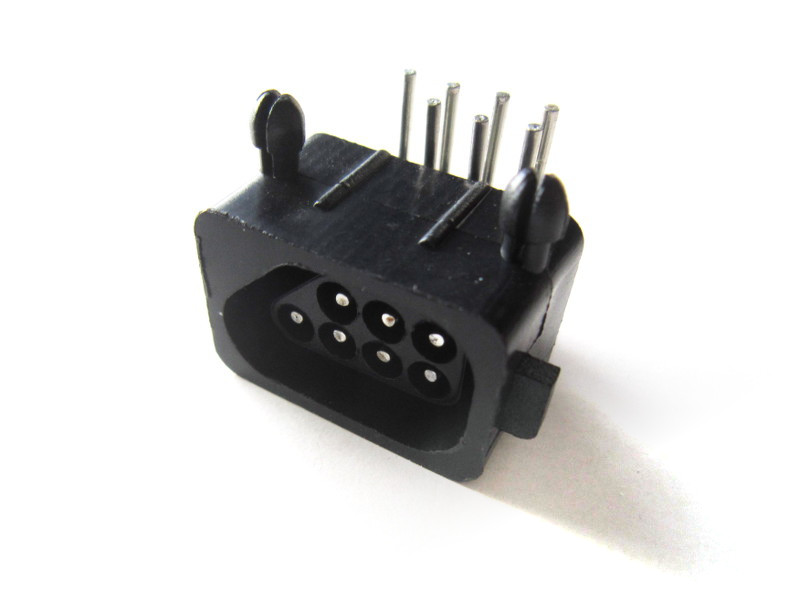
\includegraphics[width=80mm, keepaspectratio]{figures/7pin-connector} %110
		\caption{NES kontroller csatlakozó}
		\label{fig:7PIN-Port}
	\end{figure}
	
	Ebből a hét lábból kettőnek csak rögzítési szerepe van, kettő a tápellátásért felelős és a maradék három lábon keresztül történik a kontrollerben található regiszter olvasása, vezérlése és a működési órajel küldése. A kártyára ebből a csatlakozóból kettőt helyeztem el a kooperatív játékok végett. A kontroller portok sematikus ábráját (schematic) \aref{sec:DAC-controllers} függelékben láthatjuk.
	
	A pcb-n két gomb is helyet kapott az egyik az FPGA és ezáltal a NES reset gombja (RST), a másik pedig az FPGA újrakonfigurálását elindító nyomógomb (PROG). Az RST gomb pergésmentesítésért az FPGA a felelős. Ezek mindegyikét \aref{sec:OSC-JTAG} függelékben láthatjuk. 
	
\section{MicroSD kártya}
	
	A MicroSD kártya csatlakozót teljes interfésszel tudtam implementálni, mivel az FPGA-nak még sok szabad I/O lába maradt. Ez azt jelenti hogy teljes SD kártya protokollt is megtudok valósítani a NES fejlesztő kártyán, az egyszerűbb soros SPI kommunikációt mellett/helyett. A MicroSD kártya segéd áramkörét \aref{sec:HDMI-MicroSDcard} függelék sematikus rajzán láthatjuk. 
	
	Itt érdemes az áramkör ki-bekapcsolásáért felelős P-Mosfet-es áramkört megnézni, ez azért szükséges, mert a fent említett két protokoll közötti váltáshoz áramtalanítanunk kell az csatlakozót. A tápellátás elvétele mellet a felhúzó ellenállások tápellátását is elvesszük kikapcsolás során. Egyedül a CD kártya detektáló lábtól nem vesszük el, mivel ez csak azt jelzi, hogy van-e SD kártya a csatlakozóban (nem része a fent említett kommunikációs protokolloknak). Ezt be/ki kapcsolási eseményt az FPGA egy I/O lábának segítségével kontrollálhatjuk.
	
	Az FPGA védelme érdekében elhelyeztem a az SD kártya CLK lábára egy 33 $\Omega$-os soros ellenállást, ezt a PCB layout tervezése során a lehető legközelebb helyeztem el az FPGA-hoz.  
	
\section{FPGA konfigurációs módok}
	
	A NES kártyának is, a LOGSYS Spartan-6 FPGA kártyához hasonló módon \cite{spatan6} két konfigurációs módja van. Az FPGA-t felprogramozhatjuk a fejlesztőportban található JTAG interfész segítségével, illetve felkonfigurálhatja saját magát a kártyán található soros FLASH memóriából is. A konfigurációs módok között egy rövidzár segítségével (jumper) válthatunk a LOGSYS-es kártyához hasonlóan. Ennek működését \aref{tab:FPGA-config} táblázatban olvashatjuk, illetve \aref{sec:FPGA-BANKS} függelékben láthatjuk.       
	
	\begin{table}[H]
		\footnotesize
		\centering
		\begin{tabular}{|c|c|l|}
			\hline
			\rowcolor[HTML]{C0C0C0} 
			\textbf{\begin{tabular}[c]{@{}c@{}}Jumper\\ állása\end{tabular}} & {\color[HTML]{333333} \textbf{\begin{tabular}[c]{@{}c@{}}Konfigurációs \\ mód\end{tabular}}} & \multicolumn{1}{c|}{\cellcolor[HTML]{C0C0C0}\textbf{Leírás}}                                                                                                                          \\ \hline
			\rowcolor[HTML]{FFFFFF} 
			\raisebox{-.5\height}{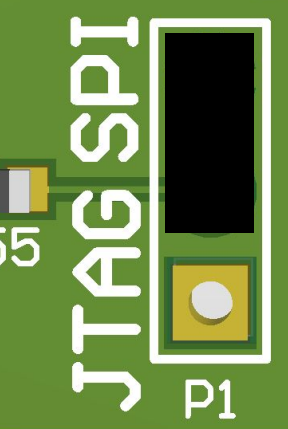
\includegraphics[width=10mm, keepaspectratio]{figures/SPI-jumper}}                                                                & JTAG                                                                                         & Az FPGA-t a JTAG interfacen keresztül kell felkonfigurálni.                                                                                                                           \\ \hline
			\rowcolor[HTML]{FFFFFF} 
			\raisebox{-.5\height}{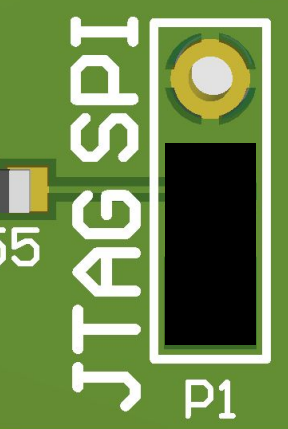
\includegraphics[width=10mm, keepaspectratio]{figures/JTAG-jumper}}                                                                & SPI                                                                                          & \begin{tabular}[c]{@{}l@{}}Az FPGA az SPI buszos soros FLASH memóriából konfigurálja \\ fel magát a tápfeszültség bekapcsolása vagy a PROG gomb \\ megnyomását követően.\end{tabular} \\ \hline
		\end{tabular}
		\caption{Fejlesztői port bekötése}
		\label{tab:FPGA-config}
	\end{table}
	
\section{Soros Flash memória}
	
	A NES kártyán egy Atmel AT25DF321A típusú, 32 Megabit-es SPI busszal rendelkező soros FLASH memóriát helyeztem el. Ez a komponens az FPGA számára konfigurációs memóriaként szolgál (tehát a NES hardverének binárisát fogja tartalmazni). Ennek a komponensnek az elhelyezése, bekötése és ezáltal működése is megegyezik a Logsys Spartan-6-os fejlesztői kártyán található Flash-el \cite{spatan6}. A soros Flash bekötését, pedig \aref{sec:SRAM-SPI-Flash} függelékben láthatjuk.
	
	%TODO fix jumper heights if you have time
\section{LOGSYS fejlesztői port}
	
	A fejlesztői port kialakítása teljes mértékben megegyezik a Logsys fejlesztő kártyán található port-al, ennek köszönhetően az FPGA felprogramozása történhet a MIT tanszéken tervezett egyedi fejlesztő kábellel. Ennek részletes bemutatása \acite{spatan6}-os dokumentáció része. A fejlesztői port kialakítását \aref{fig:DEV-port} képen látható és FPGA bekötését pedig \aref{tab:DEV-pinout} táblázatban olvasható, illetve \aref{sec:OSC-JTAG} függelékben látható. Az FPGA sikeres felkonfigurálását egy zöld LED-el jelzem (DONE). %A fejlesztői port a következő elemekből áll:
	
%	\begin{enumerate}
%		\item JTAG interfész (vörös)
%		\item Soros SPI kommunikációs interfész (zöld)
%		\item 5 V-os egyenfeszültségű táp forrás (szürke)
%	\end{enumerate}
%	
%	\begin{figure}[H]
%		\begin{minipage}[]{\textwidth}
%			\begin{minipage}[b]{0.49\textwidth}
%				\centering
%				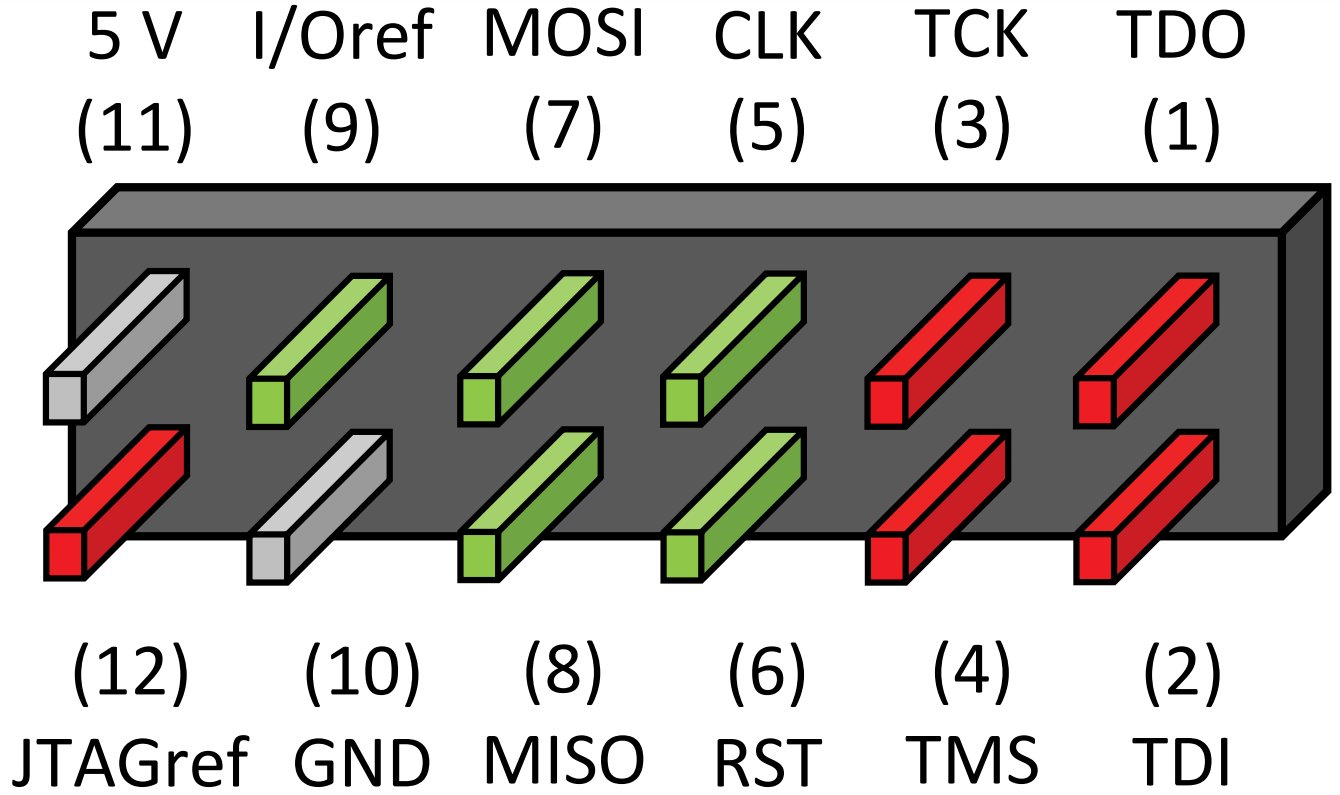
\includegraphics[width=50mm, keepaspectratio]{figures/DEV-port}
%				\captionof{figure}{Fejlesztői port kiosztása}
%				\label{fig:DEV-port}
%			\end{minipage}
%			\hfill
%			\begin{minipage}[b]{0.49\textwidth}
%				\footnotesize
%				\centering
%				\begin{tabular}{|l|l|l}
%					\cline{1-2}
%					\rowcolor[HTML]{C0C0C0} 
%					\multicolumn{1}{|c|}{\cellcolor[HTML]{C0C0C0}\textbf{jel}} & \multicolumn{1}{c|}{\cellcolor[HTML]{C0C0C0}{\color[HTML]{333333} \textbf{Irány}}} & \multicolumn{1}{c}{\cellcolor[HTML]{C0C0C0}\textbf{FPGA láb}} \\ \hline
%					\rowcolor[HTML]{FFFFFF} 
%					MOSI                                                       & bemenet                                                                            & \multicolumn{1}{l|}{\cellcolor[HTML]{FFFFFF}P104}             \\ \hline
%					\rowcolor[HTML]{FFFFFF} 
%					MISO                                                       & kimenet                                                                            & \multicolumn{1}{l|}{\cellcolor[HTML]{FFFFFF}P144}             \\ \hline
%					CLK                                                        & bemenet                                                                            & \multicolumn{1}{l|}{P95}                                      \\ \hline
%					RST                                                        & bemenet                                                                            & \multicolumn{1}{l|}{P94}                                      \\ \hline
%				\end{tabular}
%				\captionof{table}{Fejlesztői port bekötése}
%				\label{tab:DEV-pinout}
%			\end{minipage}
%		\end{minipage}
%	\end{figure} 		

\section{Nyomtatott áramköri terv}

A schematik megalkotását követően, a pcb tervezés következő fázisa a layout (pcb rajzolat) elkészítése. Itt természetesen figyelembe kell vennünk az eddig meghatározott célokat \ref{sec:Size}, miszerint egy kompakt hordozható eszközt tervezünk. Egy nyomtatott áramkör mérete nagyban függ a réteg felépítésétől, illetve a kiválasztott komponensek méretétől. Tehát minél több rétegből épül fel egy pcb és minél modernebb alkatrészeket használunk, annál nagyobb felületi alkatrész sűrűség érhető el. Természetesen ezekkel arányosán az ár is nő. Viszont mivel először egy prototípust fejlesztek, ezért egy kompromisszumos megoldást kellett választanom.   
		
	\subsection{Réteg beállítások}
	
	A Logsys Spartan-6-os fejlesztő kártyán már láthattuk \cite{spatan6}, hogy a választott FPGA chip TQFP tokozása miatt, két rétegű nyákon behuzalozható. Az FPGA NES kártya tervezésekor ez egy fő szempont volt, mivel így érdekes mérnöki megoldásokat kellett alkalmaznom a táp bekötése során, illetve a kártya elkészítési költségét is csökkenteni tudtam.
	
	A prototípus kártyákat a jlcpcb nevű kínai nyomtatott áramkör gyártó fogja gyártani. Ahhoz, hogy az Altium tervező program képes legyen bonyolultabb számítások (differencial pair routing) és szimulációk készítésére, a réteg felépítést meg kell adnunk a PCB-nk számára. Ez a kínai gyártó által szolgáltatott információk által \cite{jlcpcb} alakítottam ki, ez \aref{fig:Layer-stackup} ábrán látható.    
	
	\begin{figure}[H]
		\centering
		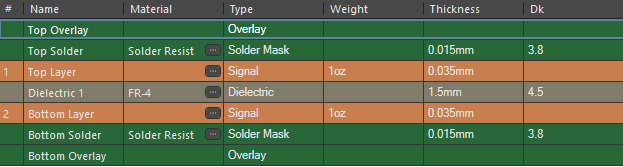
\includegraphics[width=150mm, keepaspectratio]{figures/Layer-stackup}
		\caption{Az FPGA NES kártya réteg beállításai}
		\label{fig:Layer-stackup}
	\end{figure}
	
	\subsection{Komponensek elhelyezése}
	
	A rétegbeállításokat követően, a komponensek és segéd áramköreik elhelyezése következett. Ennek segítségével tudtam meghatározni végül, hogy az FPGA mely I/O bankjaihoz/lábaihoz fogom vezetni a különböző komponensek kivezetéseit, illetve ez határozta meg pcb-m méreteit is. Az alkatrészek és segéd áramköreik rajzolatát \aref{sec:NES-components} függelékben láthatjuk, de a könnyebb áttekinthetőség érdekeben elkészítettem a következő ábrát:
	
	\begin{figure}[H]
		\centering
		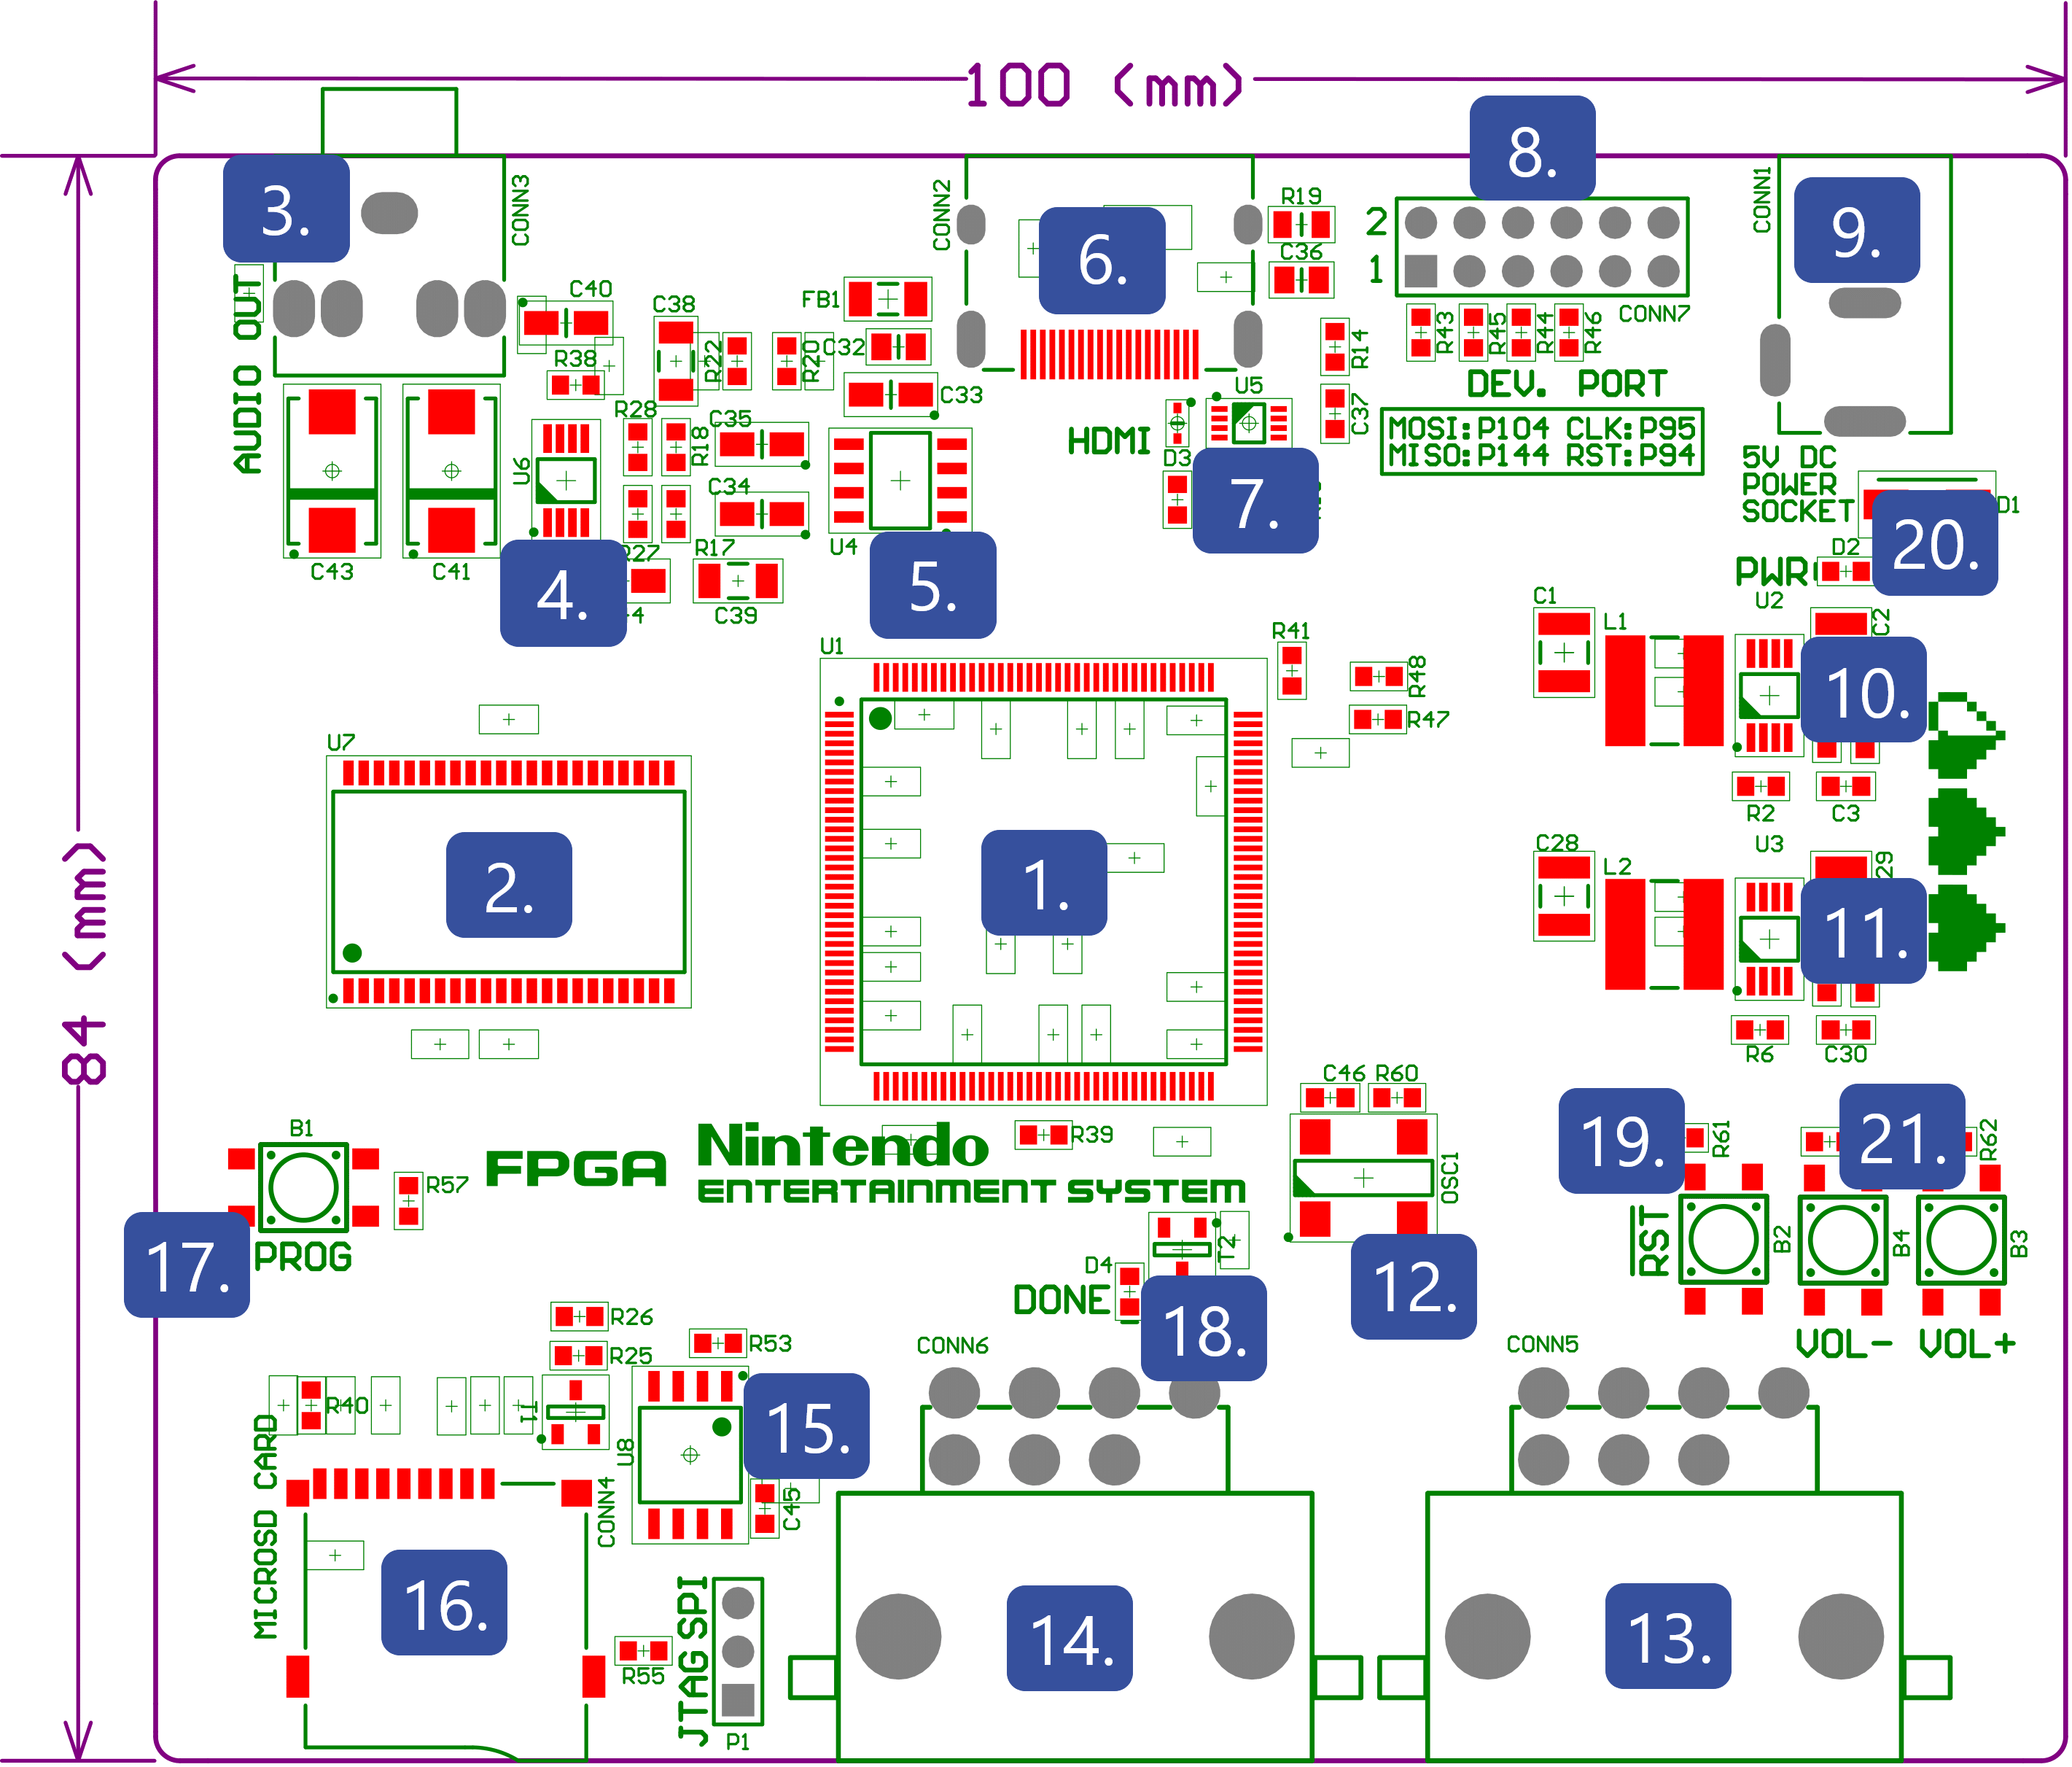
\includegraphics[width=135mm, keepaspectratio]{figures/components-top}
		\caption{A top layer alkatrész elhelyezési terve} 
		\label{fig:NES-components-top}
	\end{figure}
	
	FPGA NES kártya főbb alkotó komponensei:
	\begin{enumerate}
		\item Xilinx XC6SLX9-2TQG144C típusú FPGA
		\item 256k x 16 bites (512 kB), 10 ns-os aszinkron SRAM (Cypress CY7C1041DV33-10ZSXI)
		\item 3.5mm Jack csatlakozó (CUI SJ1-3553NG)
		\item 100mW Erősítő (TS486IST fülhallgatókhoz)
		\item Digital Analog Converter (DAC), (CS4334-KSZ)
		\item HDMI csatlakozó
		\item 2C szint illesztő (PCA9306DCUR)
		\item Csatlakozó a LOGSYS fejlesztői kábel számára
		\item 2.1mm 12 V / 5 A DC táp csatlakozó (DC10A)
		\item 3,3 V feszültséget előállító tápegység
		\item 1,2 V feszültséget előállító tápegység
		\item 50 MHz-es oszcillátor 
		\item 7 pines NES GamePAD kontroller csatlakozók anya aljzat 1
		\item 7 pines NES GamePAD kontroller csatlakozók anya aljzat 2
		\item 32 Mbites SPI buszos soros FLASH (Atmel AT25DF321A)
		\item MicroSD kártya foglalat
		\item Az FPGA újrakonfigurálását indító gomb (PROG)
		\item Az FPGA sikeres felkonfigurálását jelző LED (DONE)
		\item Az FPGA kézi reset gomja (RSTn)
		\item A bekapcsolt tápfeszültséget jelző LED (PWR)
		\item A NES hangerő szabályzó gombjai (VOL-, VOL+)
	\end{enumerate}
	
	Mivel kézi forrasztással és hőfúvó segítségével fogjuk a kártyát összeállítani, ezért törekedtem arra, hogy az összes komponens (és ezek segéd áramkörei) a előlapi (top) oldalon helyezkedjen el, illetve a hátoldalra (bottom) csak azonos méretű elemek kerüljenek. Egyedül a HDMI csatlakozó biztosítéka került a hátoldalra, ami nem 0603-as méretű lett.
	
	Ezt követően a PCB alkatrészek bekötésével foglalkoztam, itt a alsó és felső réteget is jel/föld (signal/GND) rétegként alakítottam ki. Ez azt jelenti, hogy jel vezetékeket és táp vonalak bekötését követően az egész nyák felszínén föld kitöltést hoztam létre, így növelve a jelek integritását. A alsó és a felső föld rétegeket, pedig via-k segítségével kötöttem össze (via stiching). A két rétegemet egyszerre \aref{sec:FPGA-nes-transparency} függelékben láthatjuk, az itt használt réteg ábrázolási mód az Altium designer átlátszó 2D módja, amely betekintést enged a föld kitöltések alá. A felső réteg jeleit és komponensek pad-jei vörös színnel vannak jelölve, a alsó rétegé pedig kék színnel.
	
	\subsection{HDMI adatvonalainak bekötése}
	
	A HDMI vonalak kialakításáról már \aref{sec:HMI-I2C} fejezet során olvashattunk. Viszont mivel a réteg kialakítás során a két rétegű megvalósítást választottunk és a PCB gyártó (jlcpcb) nem biztosít két réteg esetén impedancia kontrollálásra réteg felépítést. Ezért a HDMI szabványban leírt 100 $\Omega$-os impedancia különbséget (15\% os toleranciával) csak egy speciális differenciális pár bekötés típussal tudjuk biztosítani. Ez a típus a Dual Strip Coplanar Waweguide Grounded, ez azt jelenti, hogy differenciális pár bekötés mellett figyelnünk kell arra is, hogy a pár jobb és bal oldalán fix távolságra föld kitöltést helyezzünk el. Az itt található két réteg földjét előre meghatározott távolságokon via fence-szel látjuk el (ezt az elrendezést \aref{fig:coplanar} ábrán láthatjuk). A via-k közti maximális távolságot a következő képlettel számolhatjuk ki:
	
	\begin{align}
		\label{mat:via-distance}	
		S(via) = \frac{\lambda}{20} = \frac{c}{20 * f * \sqrt[]{\epsilon_r}}
	\end{align}   
	
	Az \ref{mat:via-distance} képletben található $\lambda$ a differenciális jelünk hullámhossza (a részletesebb képletben pedig: c a fény terjedési sebessége, f a jelünk frekvenciája, $\epsilon_r$ pedig az anyag dielektromos állandója). A mi esetünkben ezen a vezeték páron 250 Mhz-es jeleket fogunk küldeni, ennek hullámhossza körülbelül 1,151 m, ebből kiszámított két via közti maximális távolság 0.058 m (ennél természetesen választhatunk kisebb értéket is).
	
	\begin{figure}[H]
		\centering
		\includegraphics[width=90mm, keepaspectratio]{figures/coplanar}
		\caption{Dual Strip Coplanar Waweguide Grounded felépítése} 
		\label{fig:coplanar}
	\end{figure}
	
	Az Altium designer segítségével van lehetőségem a GND réteg és vezető pár közti távolság kiszámítására (később az ecad szoftver ez alapján fogja elhelyezni a vezetékeket). Ezek a beállítások az alábbi ábrán láthatók:      
	
	\begin{figure}[H]
		\centering
		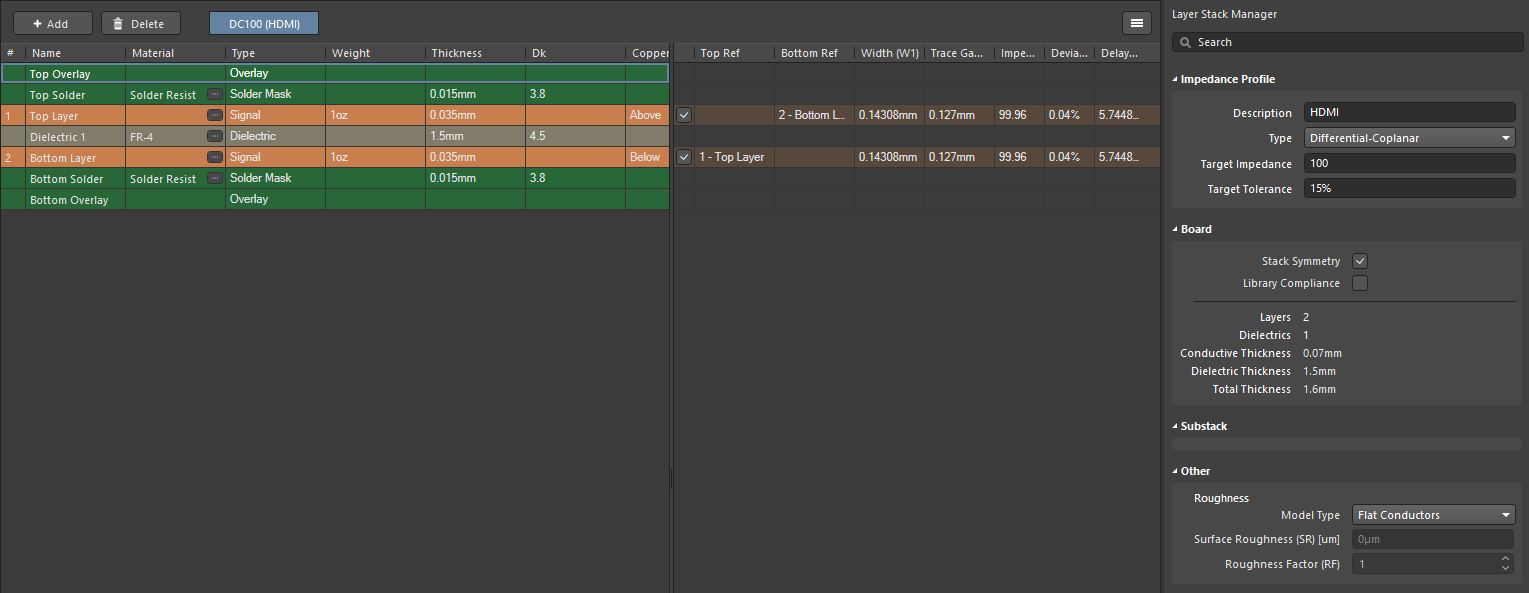
\includegraphics[width=150mm, keepaspectratio]{figures/Impedance-control}
		\caption{Coplanar differential pair routings Altium beállításai}
		\label{fig:Impedance-control}
	\end{figure}
	
	A FPGA NES kártya HDMI jeleinek bekötésére 2,75 mm-es via fence méretet választottam (körülbelül a fentebb kiszámolt érték 20-ad része) ez részletesen \aref{fig:HDMI-Differencial-pair-routing} ábrán látható, amely \aref{sec:FPGA-nes-transparency} függelékből lett kiemelve.
	
	\begin{figure}[H]
	\centering
	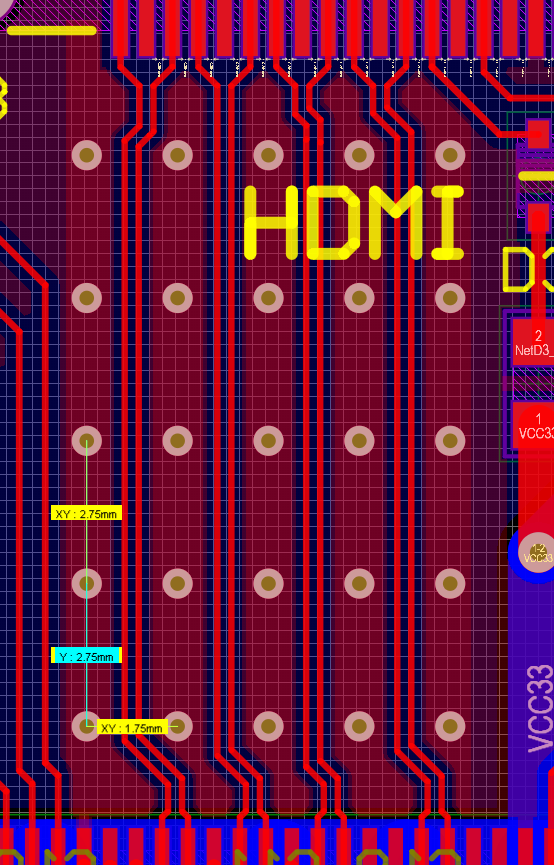
\includegraphics[width=82mm, keepaspectratio, angle=90]{figures/HDMI-Differencial-pair-routing}
	\caption{A HDMI adatvonalainak bekötése}
	\label{fig:HDMI-Differencial-pair-routing}
	\end{figure}
	
	\subsection{FPGA táp vonalak kialakítása}
	
	Ahhoz, hogy a Spartan-6-os FPGA chip-et két rétegen teljes mértékben ki tudjuk használni egy speciális tápellátási módszerhez kellet folyamodnunk (Logsys-es fejlesztő kártya táp vonalai is hasonlóan vannak kialakítva). Ennek alapja az volt, hogy az alsó oldalról érkezik a 3.3 V és az 1.2 V-is. A 3.3 V-ot az FPGA lábai alatt végig vezetjük (innen indul ki a többi 3.3 V-os komponens tápellátást is) egy helyen be engedve az 1.2 V-ot a belső magja számára. Ezzel a rendszerrel az előnye, hogy így az összes csatoló (coupling) és hidegítő (bulk) kapacitás az FPGA alatt kaphat helyet, ezzel szabadon tartva a top réteget az FPGA I/O bankjainak és JTAG interfészének bekötésére.
	
	\begin{figure}[H]
		\centering
		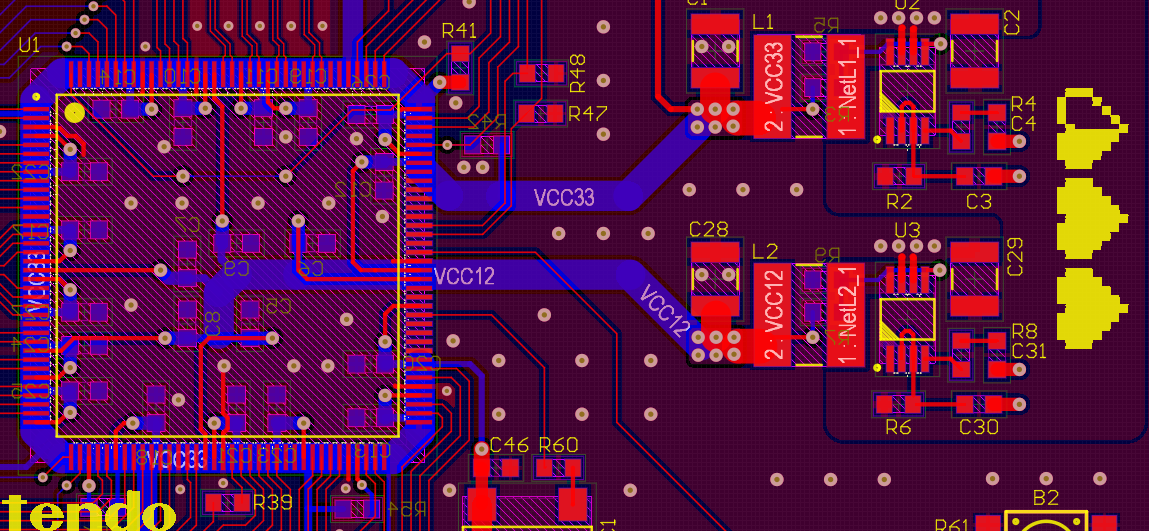
\includegraphics[width=150mm, keepaspectratio]{figures/FPGA-PSU-routing}
		\caption{FPGA tápellátásának kialakítása}
		\label{fig:FPGA-PSU-routing}
	\end{figure}
	
	A chip tápellátását \aref{fig:FPGA-PSU-routing} ábrán láthatjuk, a kártya teljes tápellátását pedig \aref{sec:FPGA-nes-transparency} függelékben figyelhetjük meg. 
	
	\subsection{FPGA NES 3D terve}
	
	A kártya tervezését követően, az Altium designer lehetőséget nyújt PCB 3D tervének megtekintéséhez (ez a komponensek elhelyezésénél, illetve nyák foglalatok/tokok tervezésénél is hasznos). Ez egy teljes képet nyújt a nyomtatott áramkör kialakításáról és jövőbeli kinézetéről. Az FPGA NES 3D tervét a következő (\ref{fig:PCB-3D}) ábrán láthatjuk:  
	
	\begin{figure}[H]
		\centering
		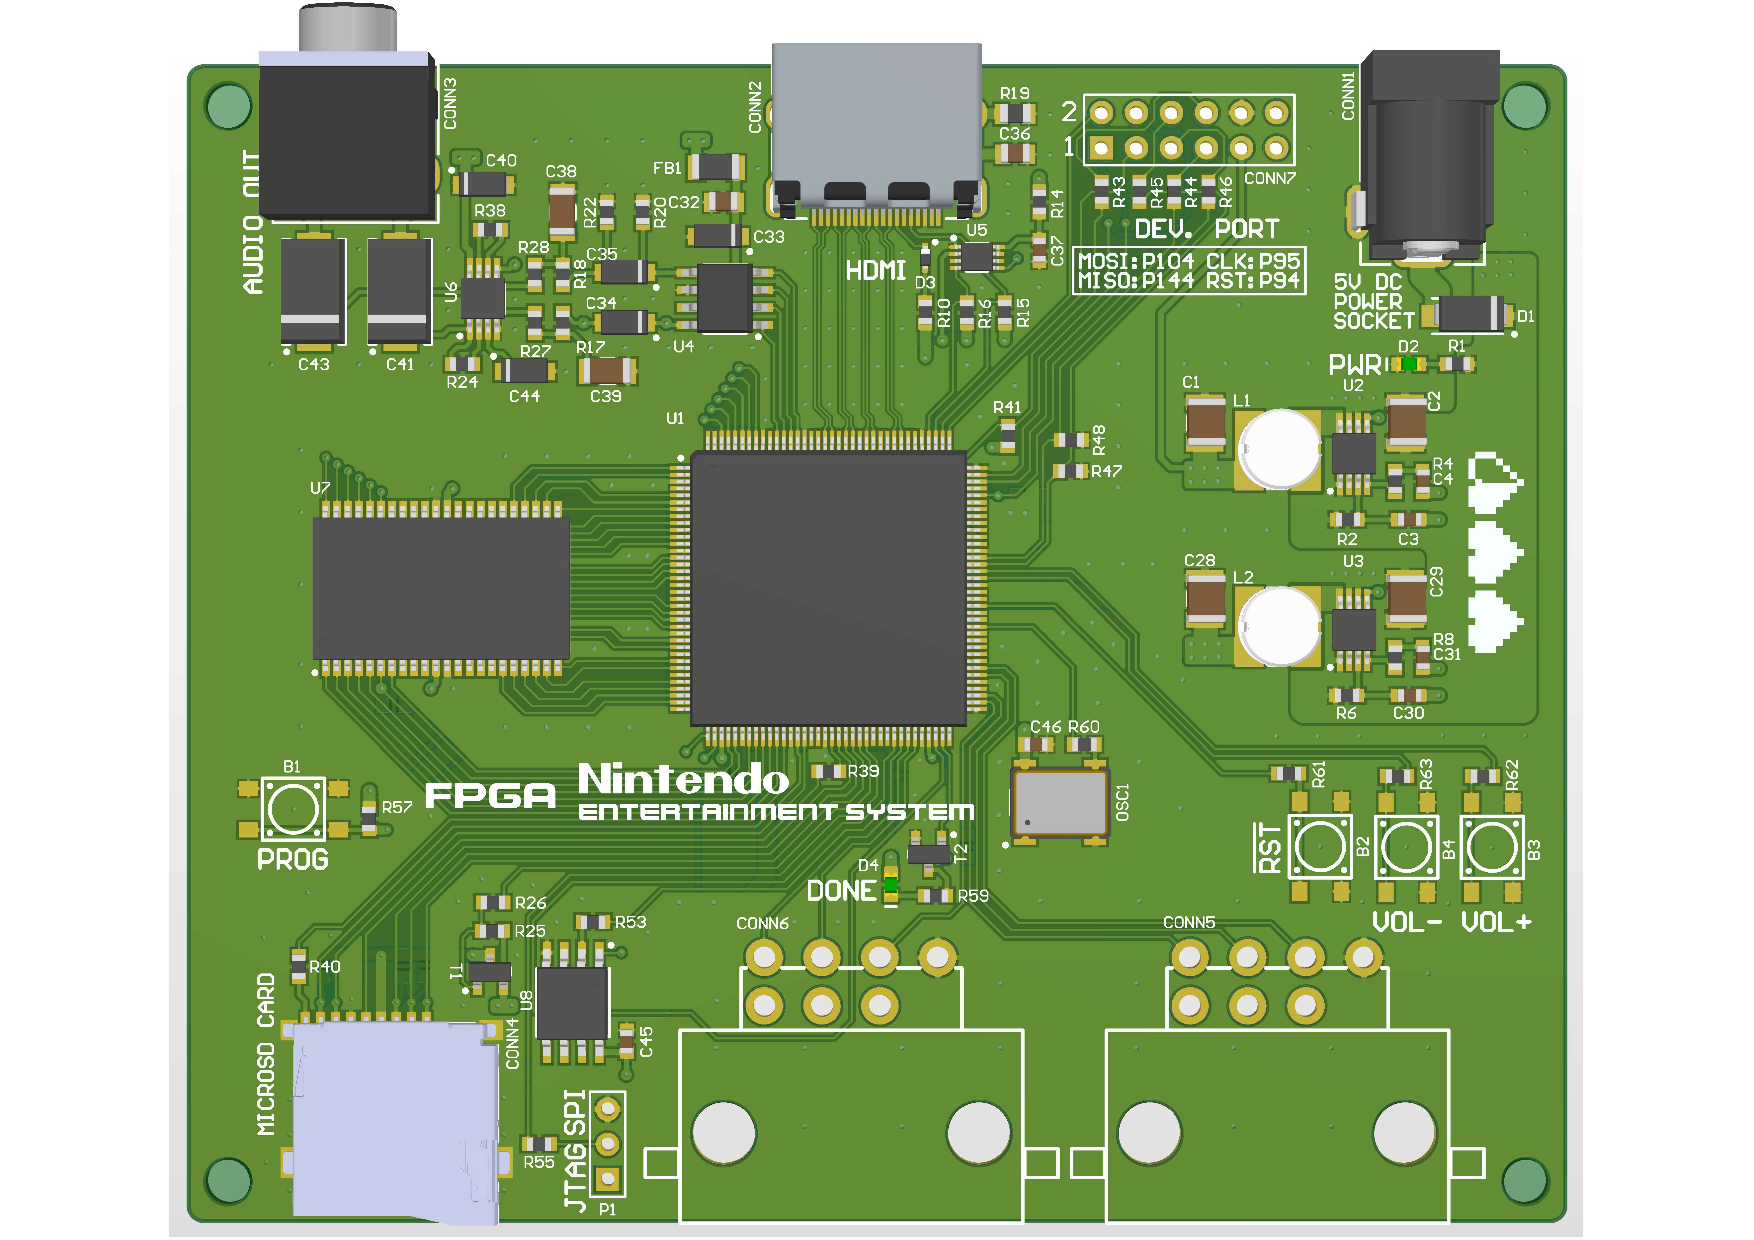
\includegraphics[width=100mm, keepaspectratio, angle=90]{figures/Top}
		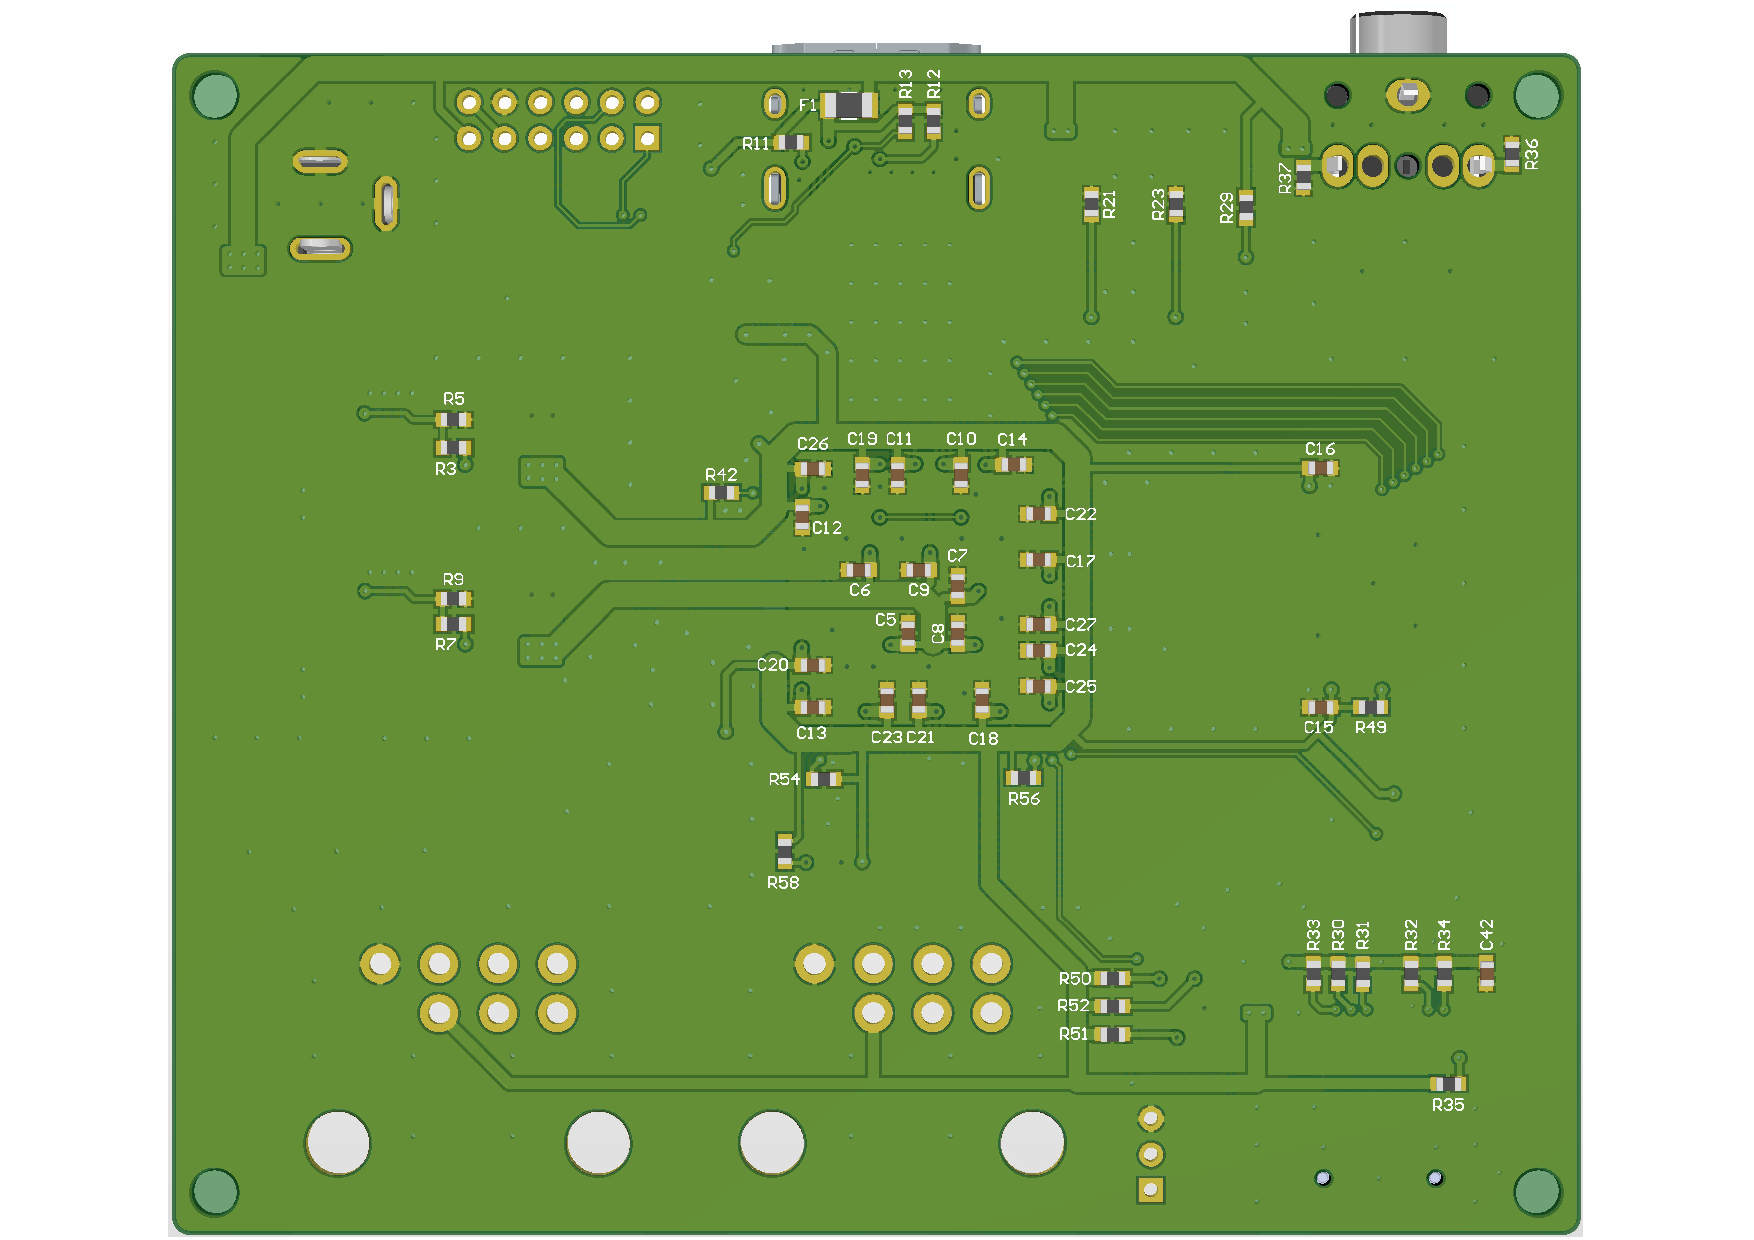
\includegraphics[width=100mm, keepaspectratio, angle=90]{figures/Bottom}
		\caption{3D PCB rajzolat} 
		\label{fig:PCB-3D}
	\end{figure}
	

	
	
	
	


\chapter{FPGA tervezés}

\section{Működési órajel választása}

\section{Picture Process Unit}

	\subsection{PPU felkészítése VGA rendeléshez}

	\subsection{Háttér rendering állapot gép}
	
	\begin{lstlisting}[style=prettyverilog]
		//rendering in visible frame
		always@(*)
		begin
		case (bgrender_state)
		IDLE:begin
		if (x_rendercntr[1:0] == 2'b01) // stay in visible frame or Pre rendering maybe should use this (& y_renderingcntr <= 9'd239 | x_rendercntr[1:0] == 2'b01 & y_renderingcntr == 9'd261)
		next_state <= NT;
		else
		next_state <= IDLE;
		end
		NT:begin
		if (x_rendercntr[9:0] == 10'd681 & y_renderingcntr == 9'd261)begin // (341*2)-1 = 681 odd frame jump to NT in the last line of PPU rendering
		if(oddframe)
		next_state <= NT;
		else
		next_state <= IDLE;
		end
		else if (x_rendercntr[9:0] == 10'd681 & y_renderingcntr <= 9'd239) // (341*2)-1 = 681 sleep just between 0-239
		next_state <= SLEEP;
		else if (x_rendercntr[9:0] == 10'd677) // (339*2)-1 = 677
		next_state <= NT;
		else if (x_rendercntr[1:0] == 2'b01) 
		next_state <= AT;
		else 
		next_state <= NT;
		end
		AT:begin
		if (x_rendercntr[1:0] == 2'b01) 
		next_state <= BG_Lsb;
		else
		next_state <= AT;
		end
		BG_Lsb:begin
		if (x_rendercntr[1:0] == 2'b01) 
		next_state <= BG_Msb;
		else
		next_state <= BG_Lsb;
		end
		BG_Msb:begin
		if (x_rendercntr[9:0] == 10'd513) // (257*2)-1 = 513
		next_state <= GB_NT_1;
		else if (x_rendercntr[1:0] == 2'b01) 
		next_state <= NT;
		else
		next_state <= BG_Msb;
		end
		GB_NT_1:begin
		if (x_rendercntr[1:0] == 2'b01) 
		next_state <= GB_NT_2;
		else
		next_state <= GB_NT_1;
		end
		GB_NT_2:begin
		if (x_rendercntr[1:0] == 2'b01) 
		next_state <= SP_Lsb;
		else
		next_state <= GB_NT_2;
		end
		SP_Lsb:begin
		if (x_rendercntr[1:0] == 2'b01) 
		next_state <= SP_Msb;
		else
		next_state <= SP_Lsb;
		end
		SP_Msb:begin
		if (x_rendercntr[9:0] == 10'b641) // (321*2)-1 = 641
		next_state <= NT;
		else if (x_rendercntr[1:0] == 2'b01) 
		next_state <= GB_NT_1;
		else
		next_state <= SP_Msb;
		end
		//PPU and CPU en off just VGA rendering goes
		SLEEP:begin
		if (x_rendercntr == 11'd1363 & y_renderingcntr == 9'd239)
		next_state <= VBLANK;
		else if (x_rendercntr == 11'd1363 & y_renderingcntr < 9'd239) // (341*4)-1 = 1363
		next_state <= IDLE;	
		else
		next_state <= SLEEP;
		end
		//I take prost-rendering line and VBlank together just one bit set in thissection
		VBLANK:begin
		if (x_rendercntr[9:0] == 10'd681 & y_renderingcntr <= 9'd260) //(341*2)-1 = 681
		next_state <= IDLE;
		else 
		next_state <= VBLANK;
		end
		default:
		next_state <= 4'bxxxx;
		endcase
		end
	\end{lstlisting}

	\subsection{Sprite rendering állapot gép}
	
	\subsection{Memória elérés}

	\subsection{Irányító regiszterek és PPU adatbusz}

\section{NES memória felépítése FPGA-ban}

\section{CPU}

\section{APU}

\section{Játék vezérlők kezelése}
%\chapter{A működéshez szükséges szoftver}

\chapter{Az FPGA NES tesztelése}

Az FPGA-s projektek tesztelésének általában három nagy fázisa van. Az első a fejlesztői környezet szimulációs rendszerében futtatott tesztek. A második ezt követően az éles hardverrel futtatott tesztek. A teszteket végeztével az eredmények kiértékelése a harmadik fázis. Ezeket a teszt folyamatokat fogom bemutatni a diplomaterv projektemen, ebben a fejezetben.

\section{Rendszer szimulációk}

A legtöbb esetben egy FPGA-s fejlesztések során a tesztelések két csoportra bonthatóak: a modul tesztekre és a teljes rendszer tesztelésére. A NES projekt esetén viszont olyan komplex változásokat és bemeneteket kellett volna időzítéspontosan megadni a különálló modul tesztekhez (teljes CPU ciklusok processzor oldali műveletei), hogy inkább közvetlenül a teljes rendszer tesztelését kezdtem el.

A rendszer teszteket az ISE-n belül található ISim szimulátorában végeztem. Ezzel képesek vagyunk szintetizálható hardverek működési szimulációjára és az implementálás utáni, úgynevezett post-implemented rendszerek szimulálására is. A szintetizálható rendszerek esetében Verilog test fixture készítésével tudjuk meghatározni a szimulált jeleinket és szimulációs órajeleinket. A NES tesztkörnyezetének írása során a VGA modult és a hozzá tartozó elemeket kivettem a rendszerből, mivel ez csak extra számítást vett volna el a szimulátortól, illetve a rendszer időzítéseinek szinkronizálását is nehezebbé tette volna (50 MHz és 250 MHz-es órajelek arányainak megtartása a rendszer órajellel).

Ahhoz, hogy a teljes NES hardveremet szimulálhassam, szimulálhatóvá kellett tennem a konzulensemtől kapott 6502-es processzor futtatható binárisát. Ezt a feladatot az UNISIM konzol alkalmazás segítségével tudtam megoldani. Ez az eszköz azt teszi lehetővé, hogy implementált modulokból post-implemented szimulációs fájlt készít. Majd ehhez egy általunk értelmezhető Verilog input és output portokkal ellátott modult illeszt, ezáltal képesek vagyunk a kapott szimulációs fájt beilleszteni egy Verilog test fixture-be. A program futtatásához \aref{fig:UNISIM}. ábrán látható beállításokat alkalmaztam.

\begin{figure}[H]
	\centering
	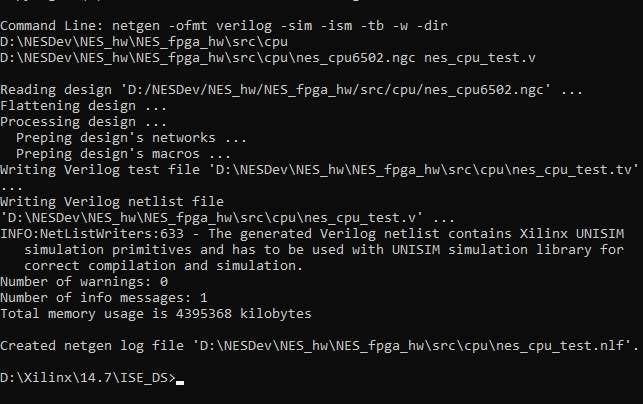
\includegraphics[width=120mm, keepaspectratio]{figures/UNISIM}
	\caption{Az UNISIM konzol alkalmazás beállításai} 
	\label{fig:UNISIM}
\end{figure}

A szimulációkhoz és későbbiekben a hardveres tesztekhez is szükségünk van arra, hogy a Karakter és Program ROM-jaink helyes adatokat tartalmazzanak. A NES játékkártyák tartalma általában egy .nes bináris fájlban áll rendelkezésre. Ez tartalmaz egy 16 bájtos fejlécet, majd a program ROM-ot, végül pedig a karakter ROM-ot. A fejléc írja le, hogy az adott játék ROM-jai mekkora területet foglalnak, illetve a játék kártya milyen mapper-t tartalmaz. A .nes fájlt egy program segítségével könnyen felbonthatjuk két bináris ROM területre, majd egy egyszerű shell script segítségével szöveges fájlba írhatjuk a kapott binárisaink tartalmát. Majd az így kapott szöveges fájlok tartalmát a \$readmemh parancs segítségével tudjuk a blokk RAM-okba tölteni. A szimulációk kezdetén a helyes működéséhez érdemes még az összes használt memória területet 0-val feltölteni. Ezeknek az inicializációknak egy részét \aref{code:filling-RAM}. hardverleírásban olvashatjuk.

\begin{lstlisting}[caption={A memória területek inicializálása a szimulációs és hardveres tesztekhez}, label={code:filling-RAM}, style=prettyverilog]
//Character ROM initialization 
initial begin
	$readmemh( "src/games/DK_chr_rom_hex.txt" , ch_rom); //Super_Mario_Bros_chr_rom.txt
end

//NT RAM initialization 
reg  [7:0] 		name_table_ram [2047:0];
integer x;
initial begin for (x=0; x<2048; x=x+1) name_table_ram[x] = 8'b0;
end\end{lstlisting}

Azt tapasztaltam, hogy nagyobb és összetettebb rendszerek szimulációja során az ISim, hosszabb időtartalmú szimulációkra nem alkalmas (nem konzisztensek a számításai). Ezáltal csak egy adott pontig tudtam a szimulációkra hagyatkozni, viszont ez pont elégnek volt ahhoz, hogy könnyen elkezdhessem a teljes rendszer hardveres tesztelését.  

\newpage
\section{Hardveres tesztek}

A diplomatervem során sikerült elkészíteni a konzulensem segítségével az első verzióját az FPGA NES kártyának. Ez \aref{fig:PCB-Assembled}. ábrán látható. \Aref{sec:fpga-nes-board-summary}. fejezet során viszont már egy javított második verziót mutattam be (ezért láthatunk némi különbséget a két kártya elrendezése között). A második verzióra javítottam a flash chip FPGA-ba huzalozásán és két extra hangerő szabályzó gombot adtam a nyákhoz.

\begin{figure}[H]
	\centering
	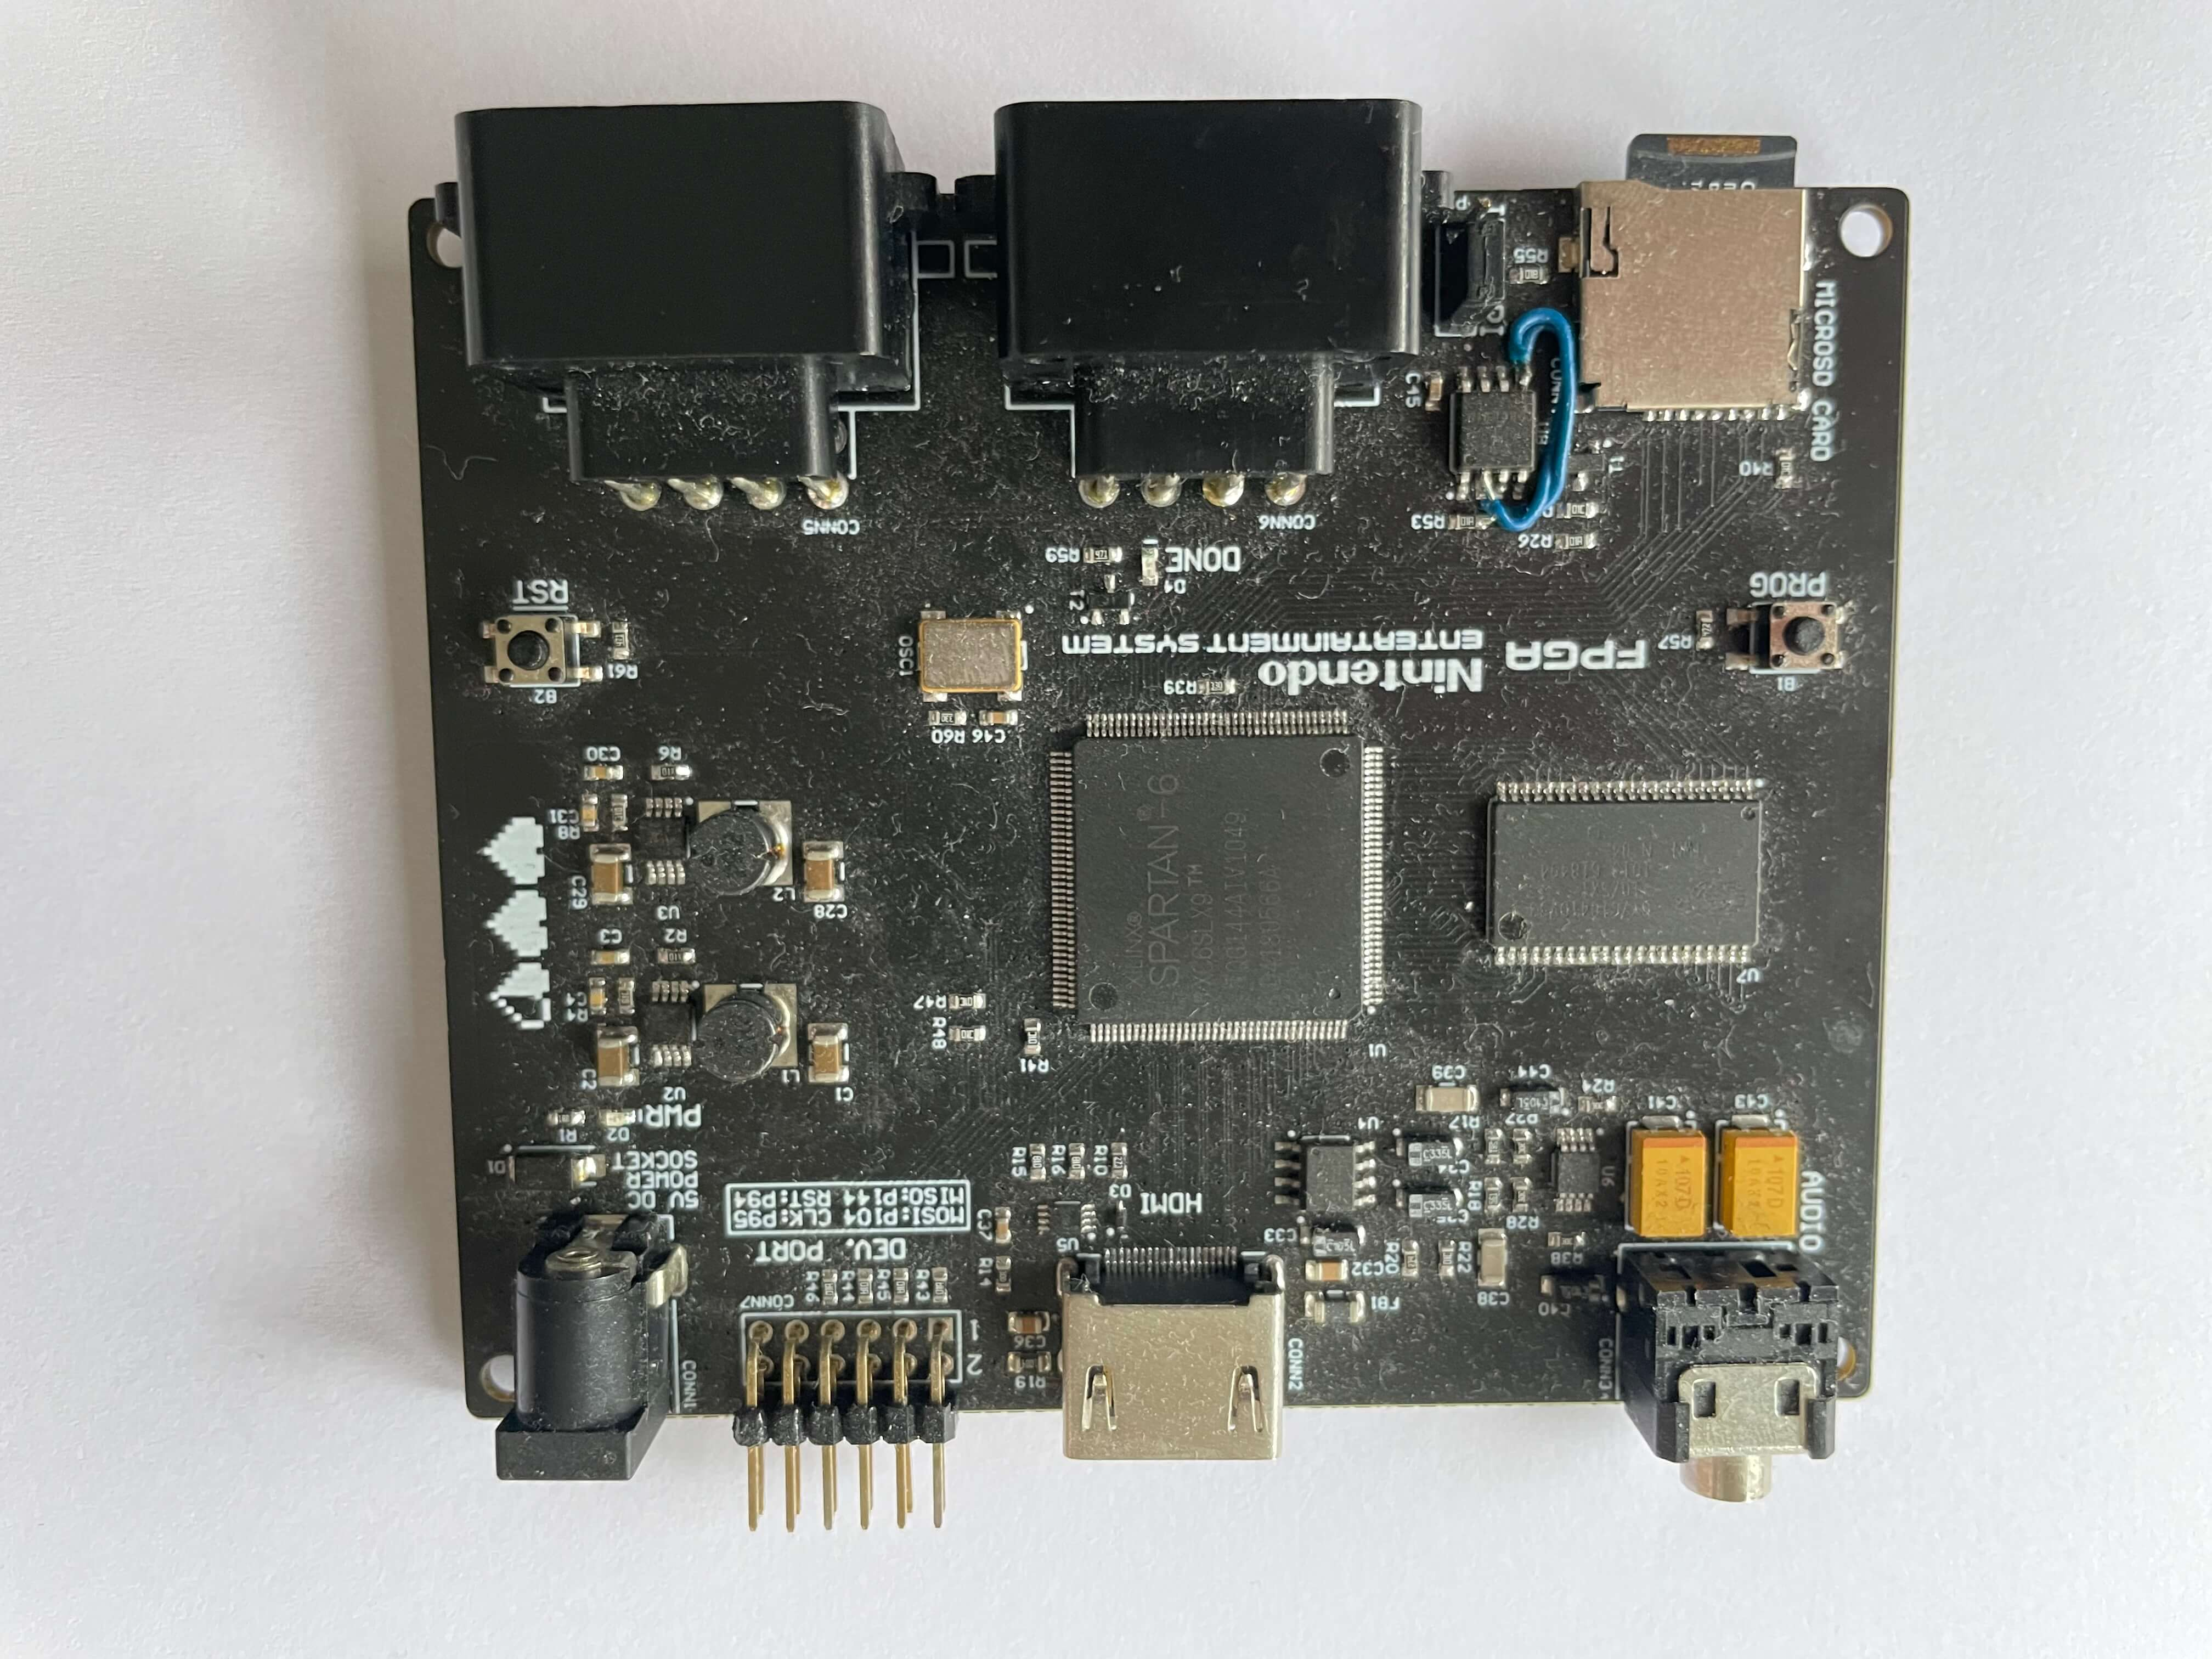
\includegraphics[width=99mm, keepaspectratio, angle=90]{figures/nes-pcb-assembled-top}
	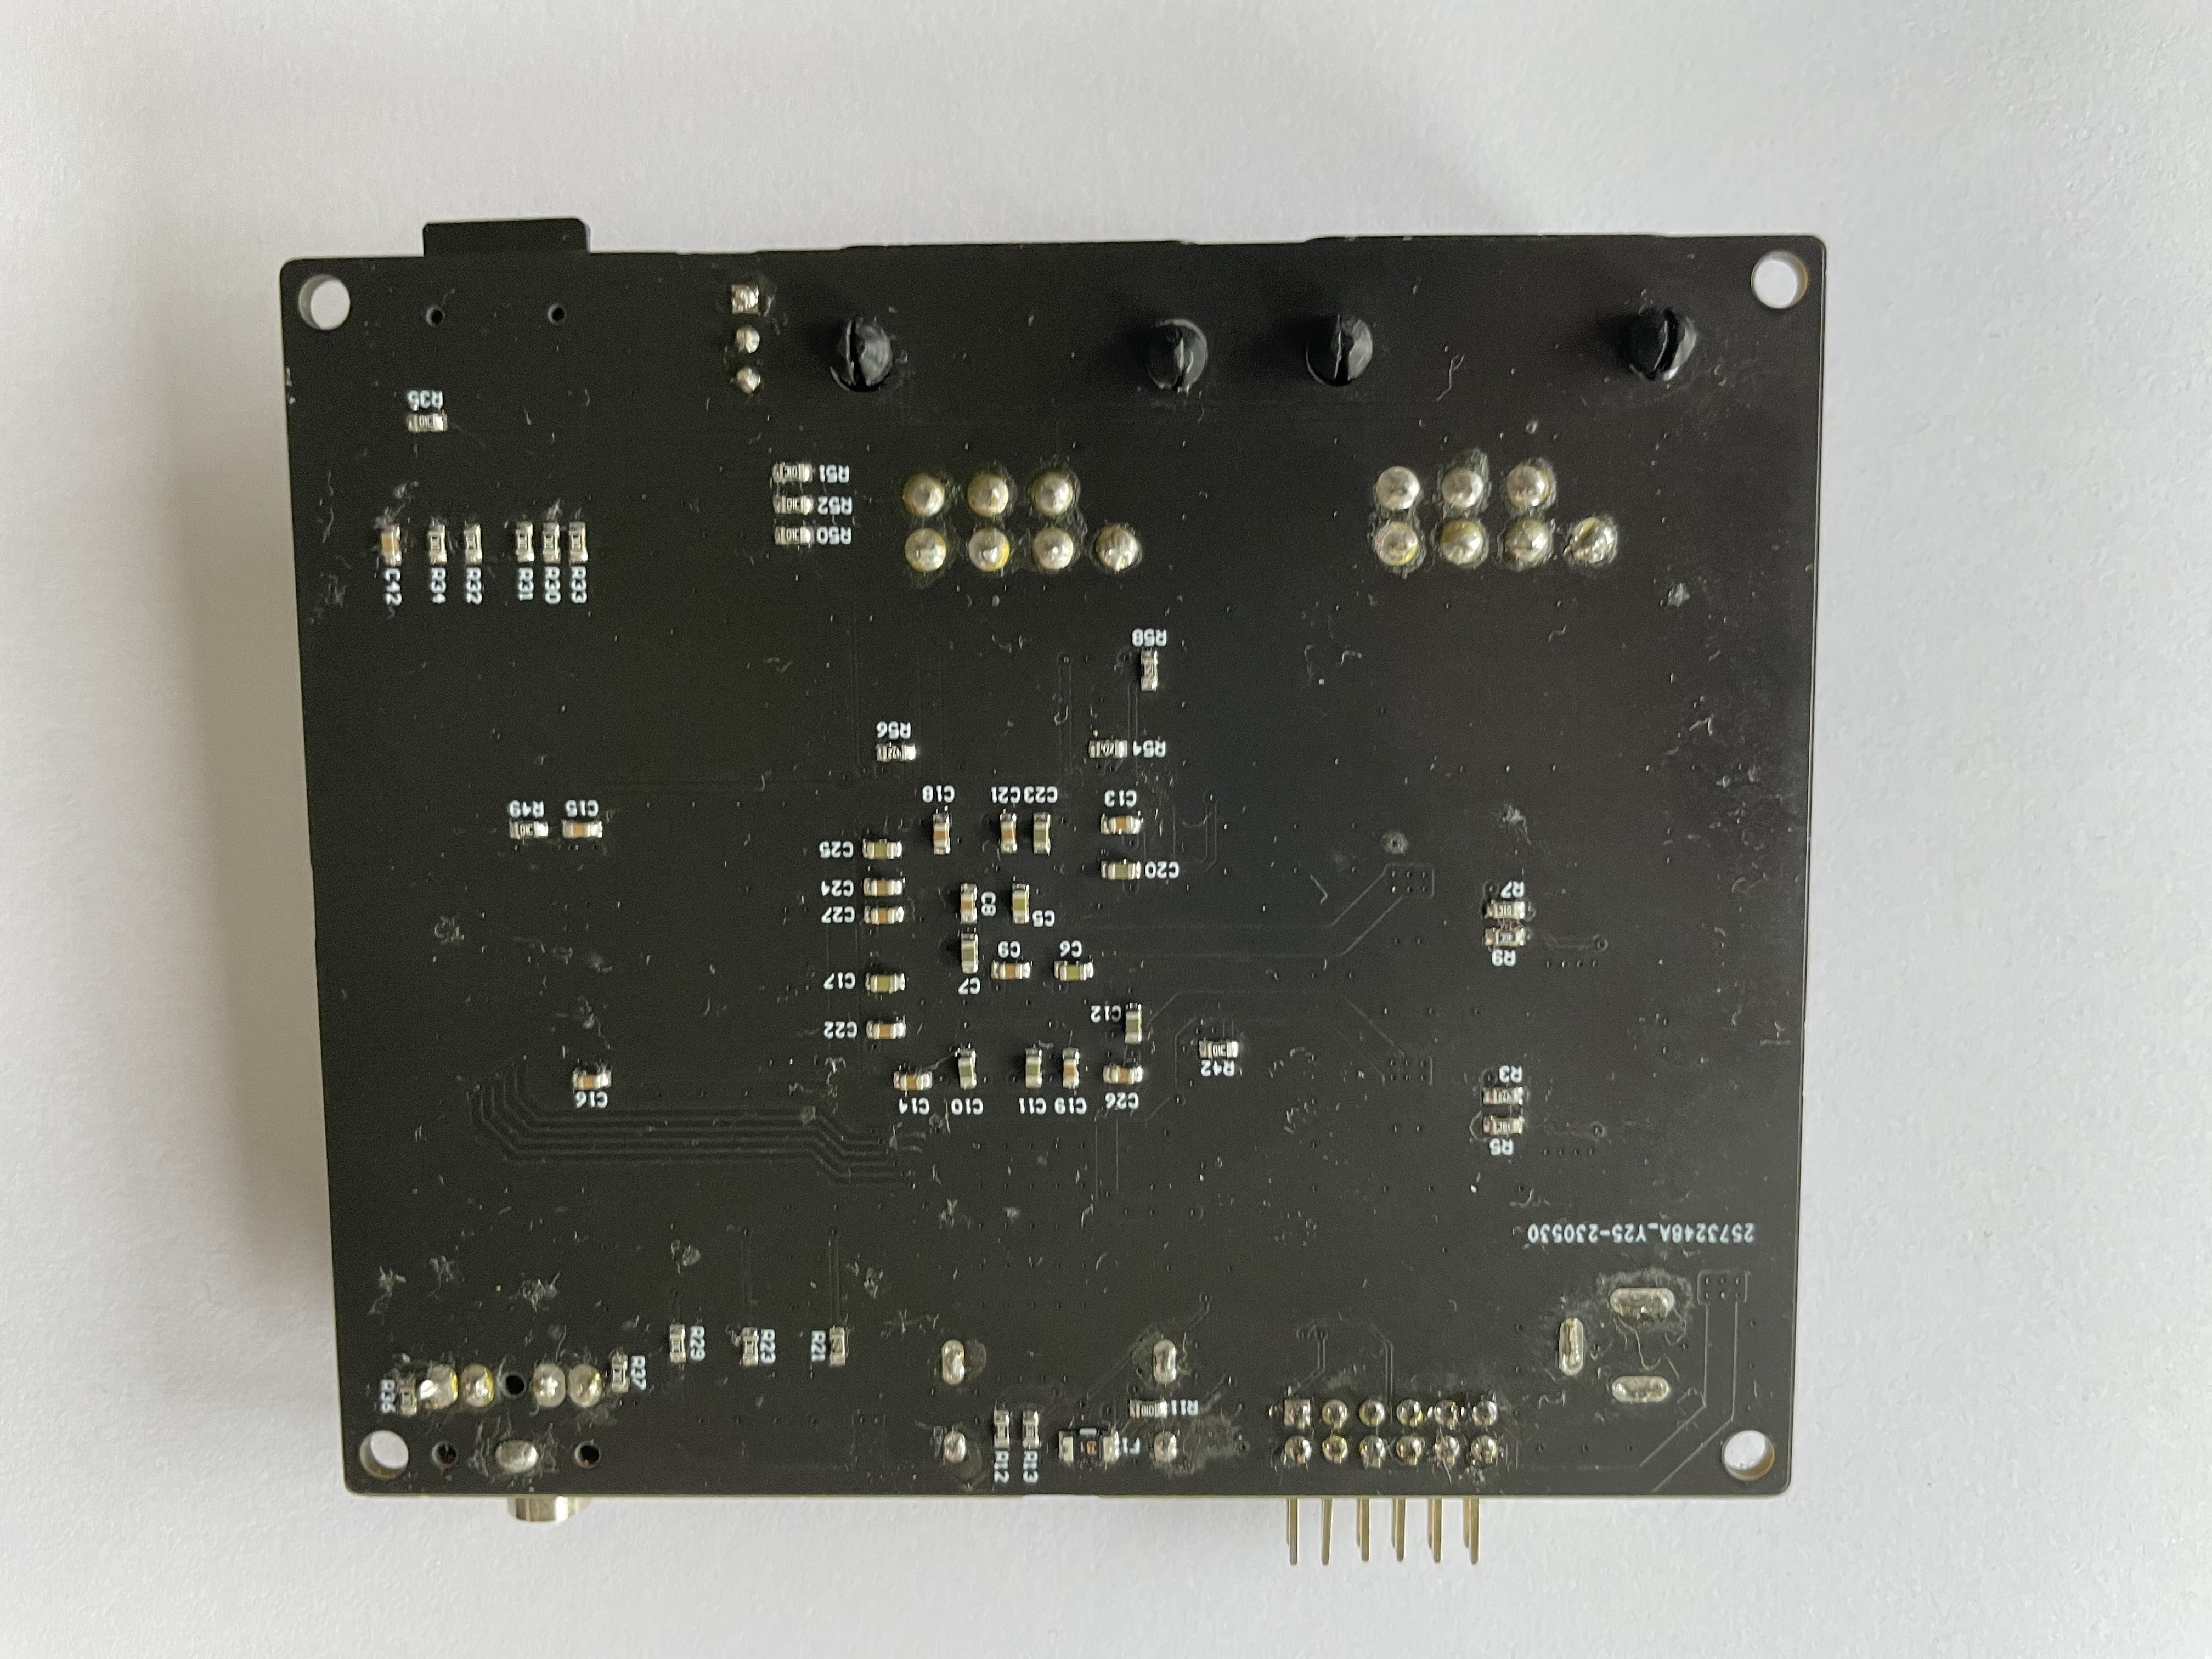
\includegraphics[width=99mm, keepaspectratio, angle=90]{figures/nes-pcb-assembled-botom}
	\caption{A kész FPGA NES kártya} 
	\label{fig:PCB-Assembled}
\end{figure}

A hardveres tesztelés során, a hardver binárisának feltöltésére a MIT-en fejlesztett, Logsys flash programozót használtam, ennek implementálását már a fentebbiekben olvashattuk (\ref{sec:logsysport}. fejezet). Az FPGA NES kártya mérési és tesztelési elrendezését \aref{fig:pcb-testing}. ábrán láthatjuk. 

A NES rendszer tesztelésére két klasszikus játékot választottam. Az első a Donkey Kong, amely egy könnyebben emulálható 16 kilobájtos program ROM-al rendelkező játék. A második pedig a NES egyik legnehezebben emulálható játéka, a Super Mario Bros. Ehhez a játékhoz hibátlanul implementált időzítésekre és helyesen kialakított PPU és CPU memória címekre van szükség. Ezt a játékot szokták legtöbbször a végső tesztként használni emulált PPU-k és CPU-k tesztelésére. A Donkey Kong tesztelését és futását \aref{fig:Donkey-start}. és \ref{fig:Donkey-level-1}. ábrákon láthatjuk. A Super Mario Bros.-t pedig futás közben \aref{fig:Super-Mario-start}. és \ref{fig:Super-Mario-world5-1}. ábrán tekinthetjük meg.
	
\begin{figure}[H]
	\centering
	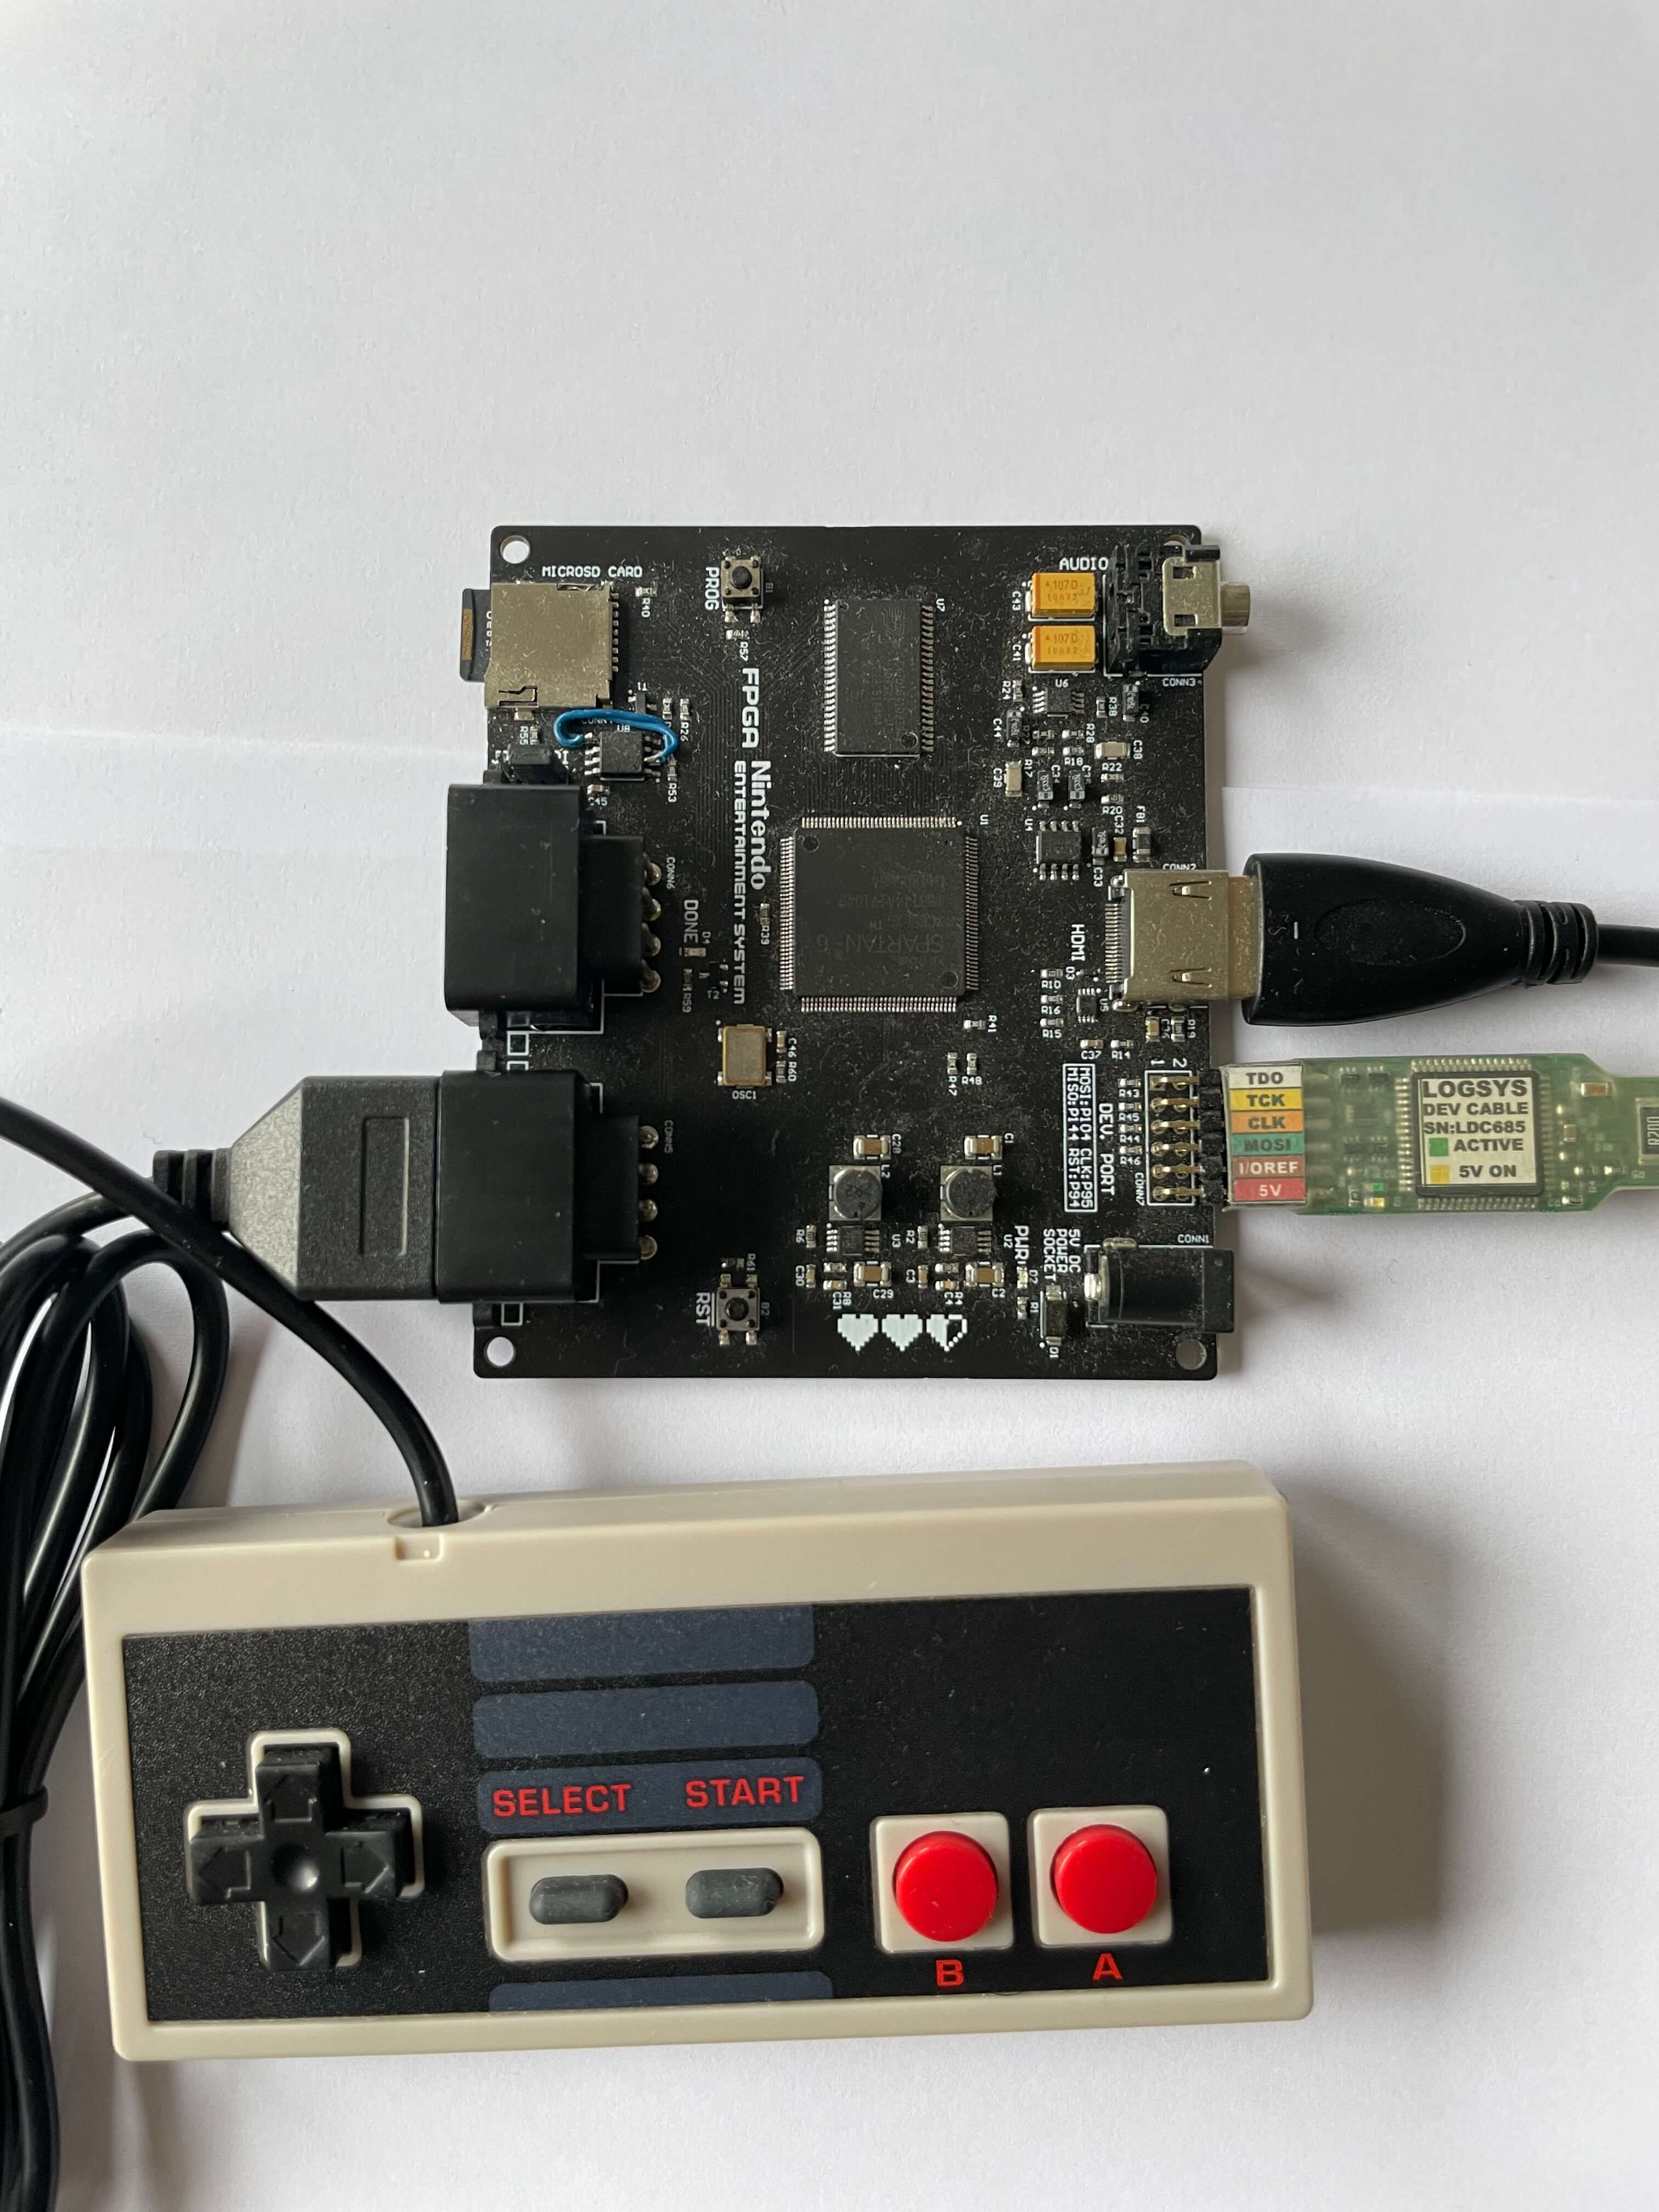
\includegraphics[width=112mm, keepaspectratio, angle=90]{figures/nes-pcb-testing}
	\caption{FPGA NES kártya mérési és tesztelési elrendezésé} 
	\label{fig:pcb-testing}
\end{figure}

\begin{figure}[H]
	\centering
	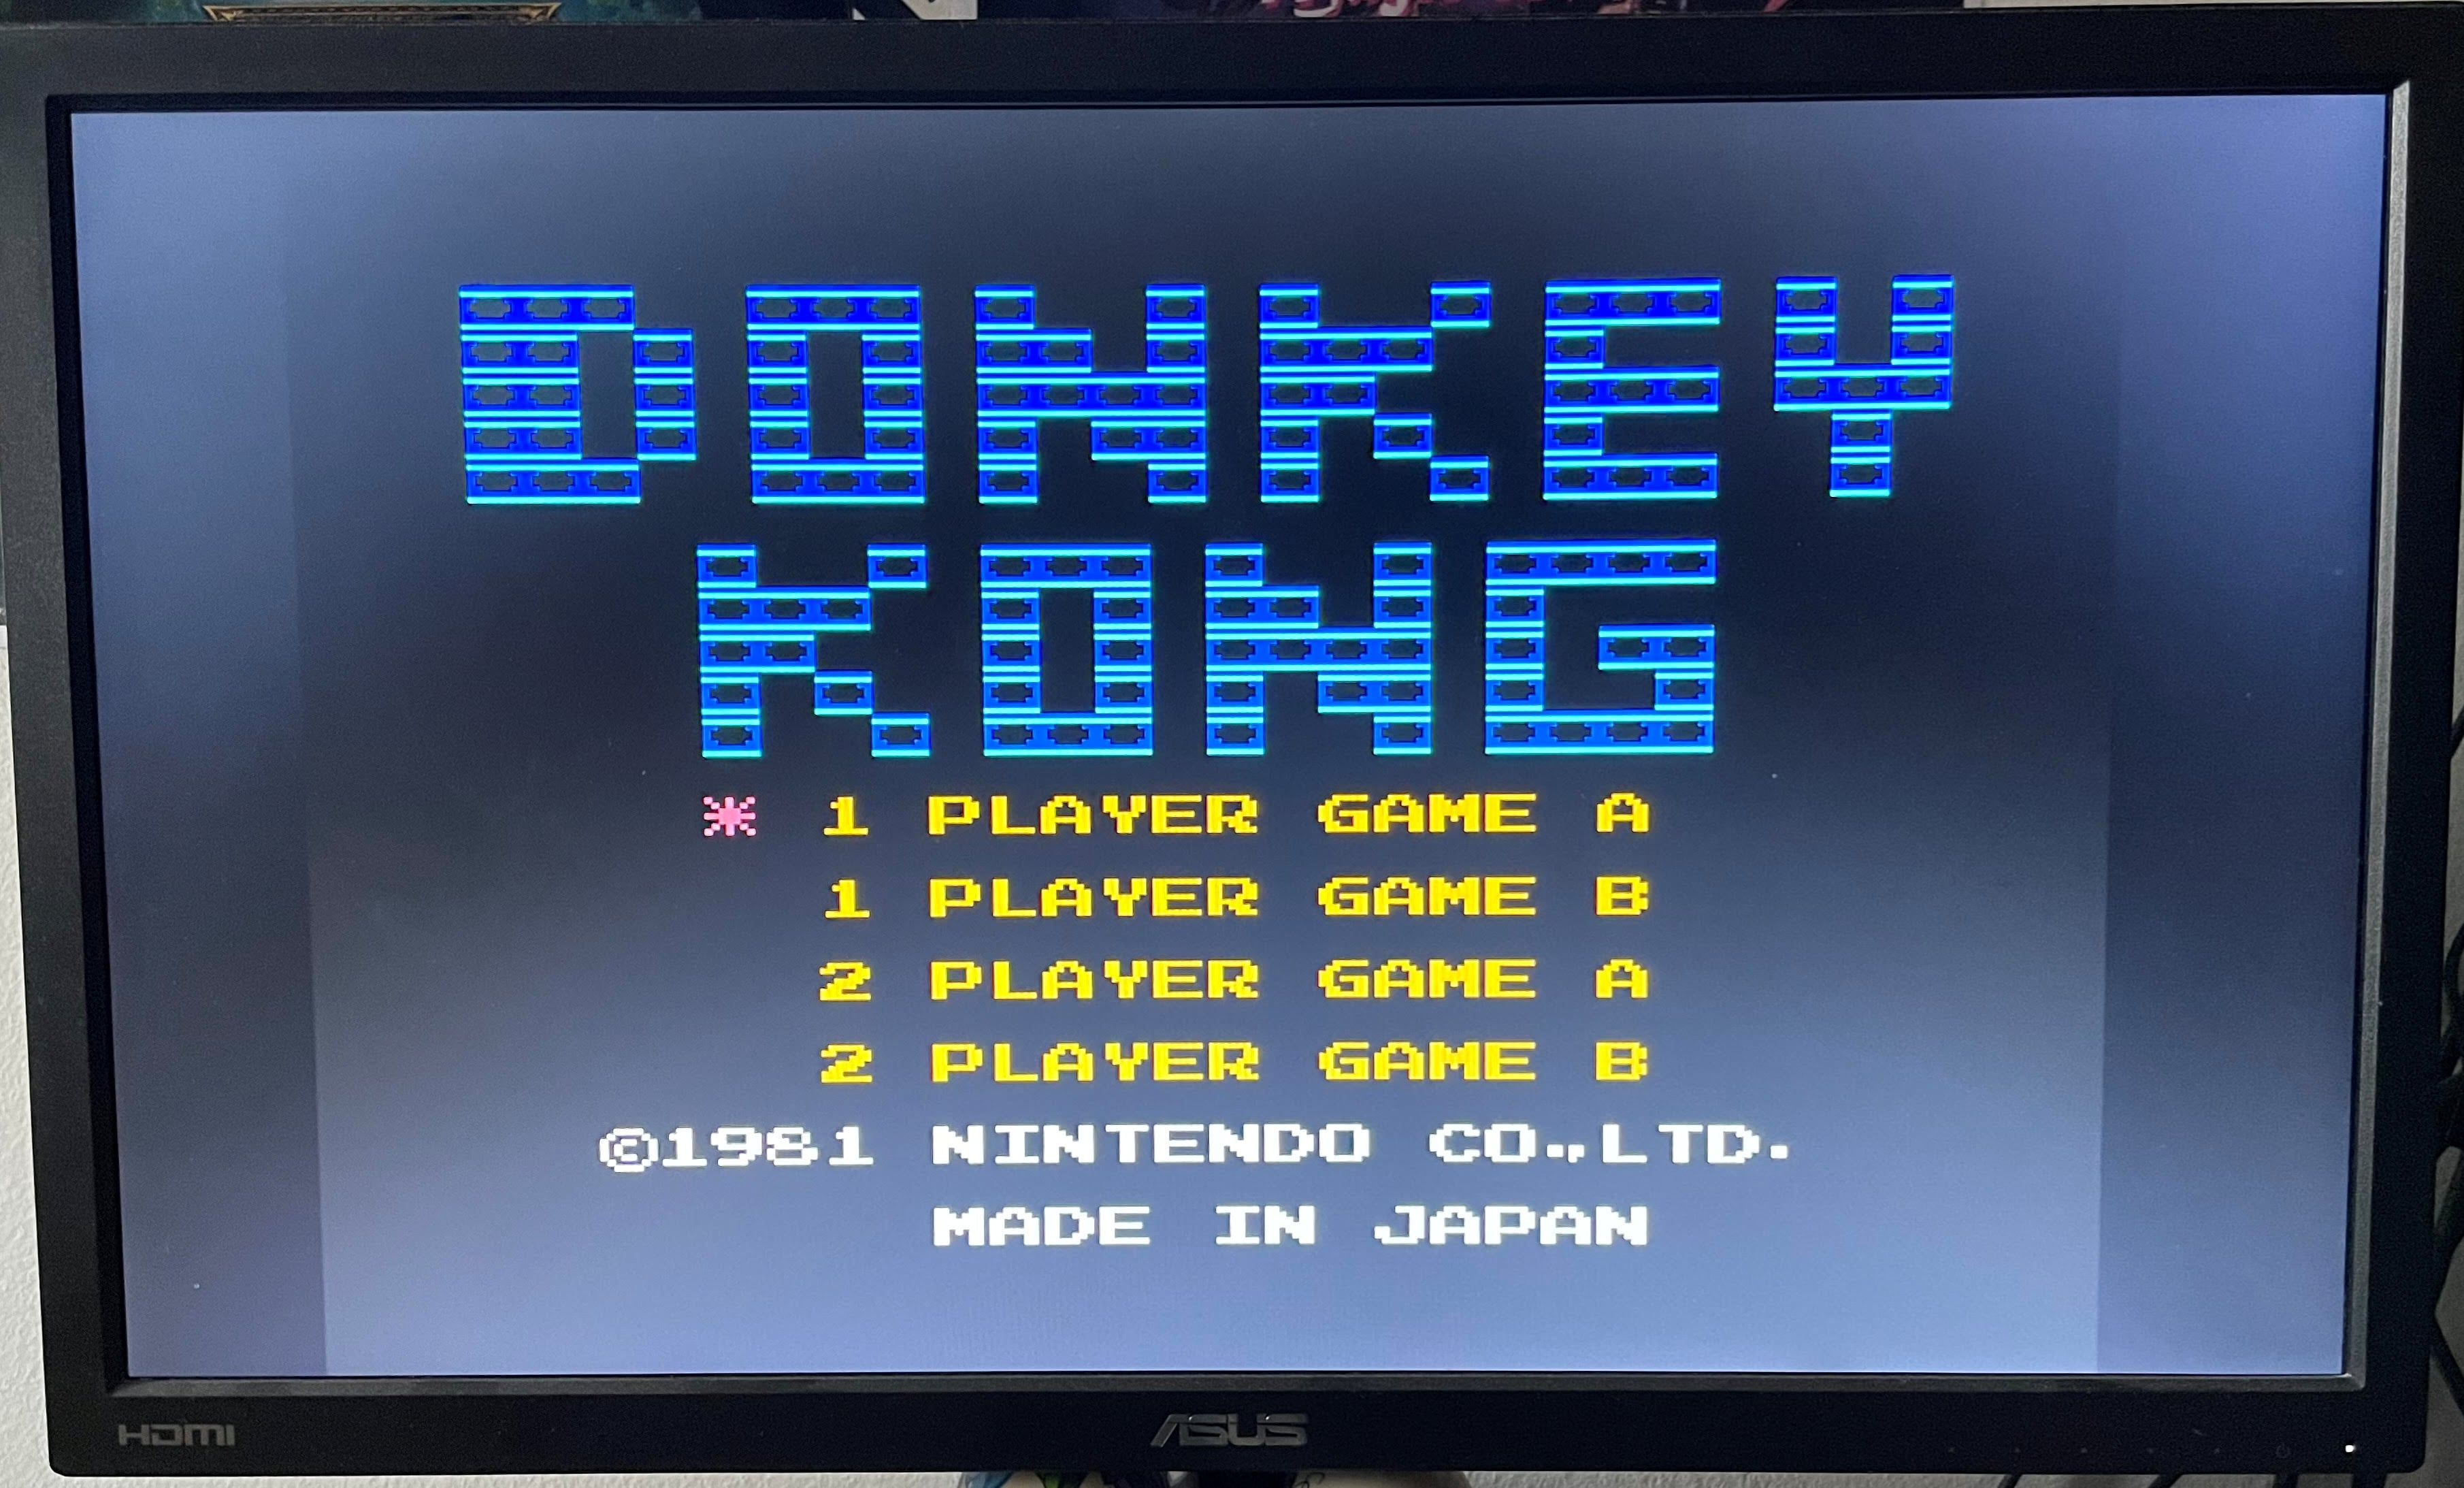
\includegraphics[width=150mm, keepaspectratio]{figures/Donkey-start}
	\caption{A Donkey Kong kezdő képernyője} 
	\label{fig:Donkey-start}
\end{figure}

\begin{figure}[H]
	\centering
	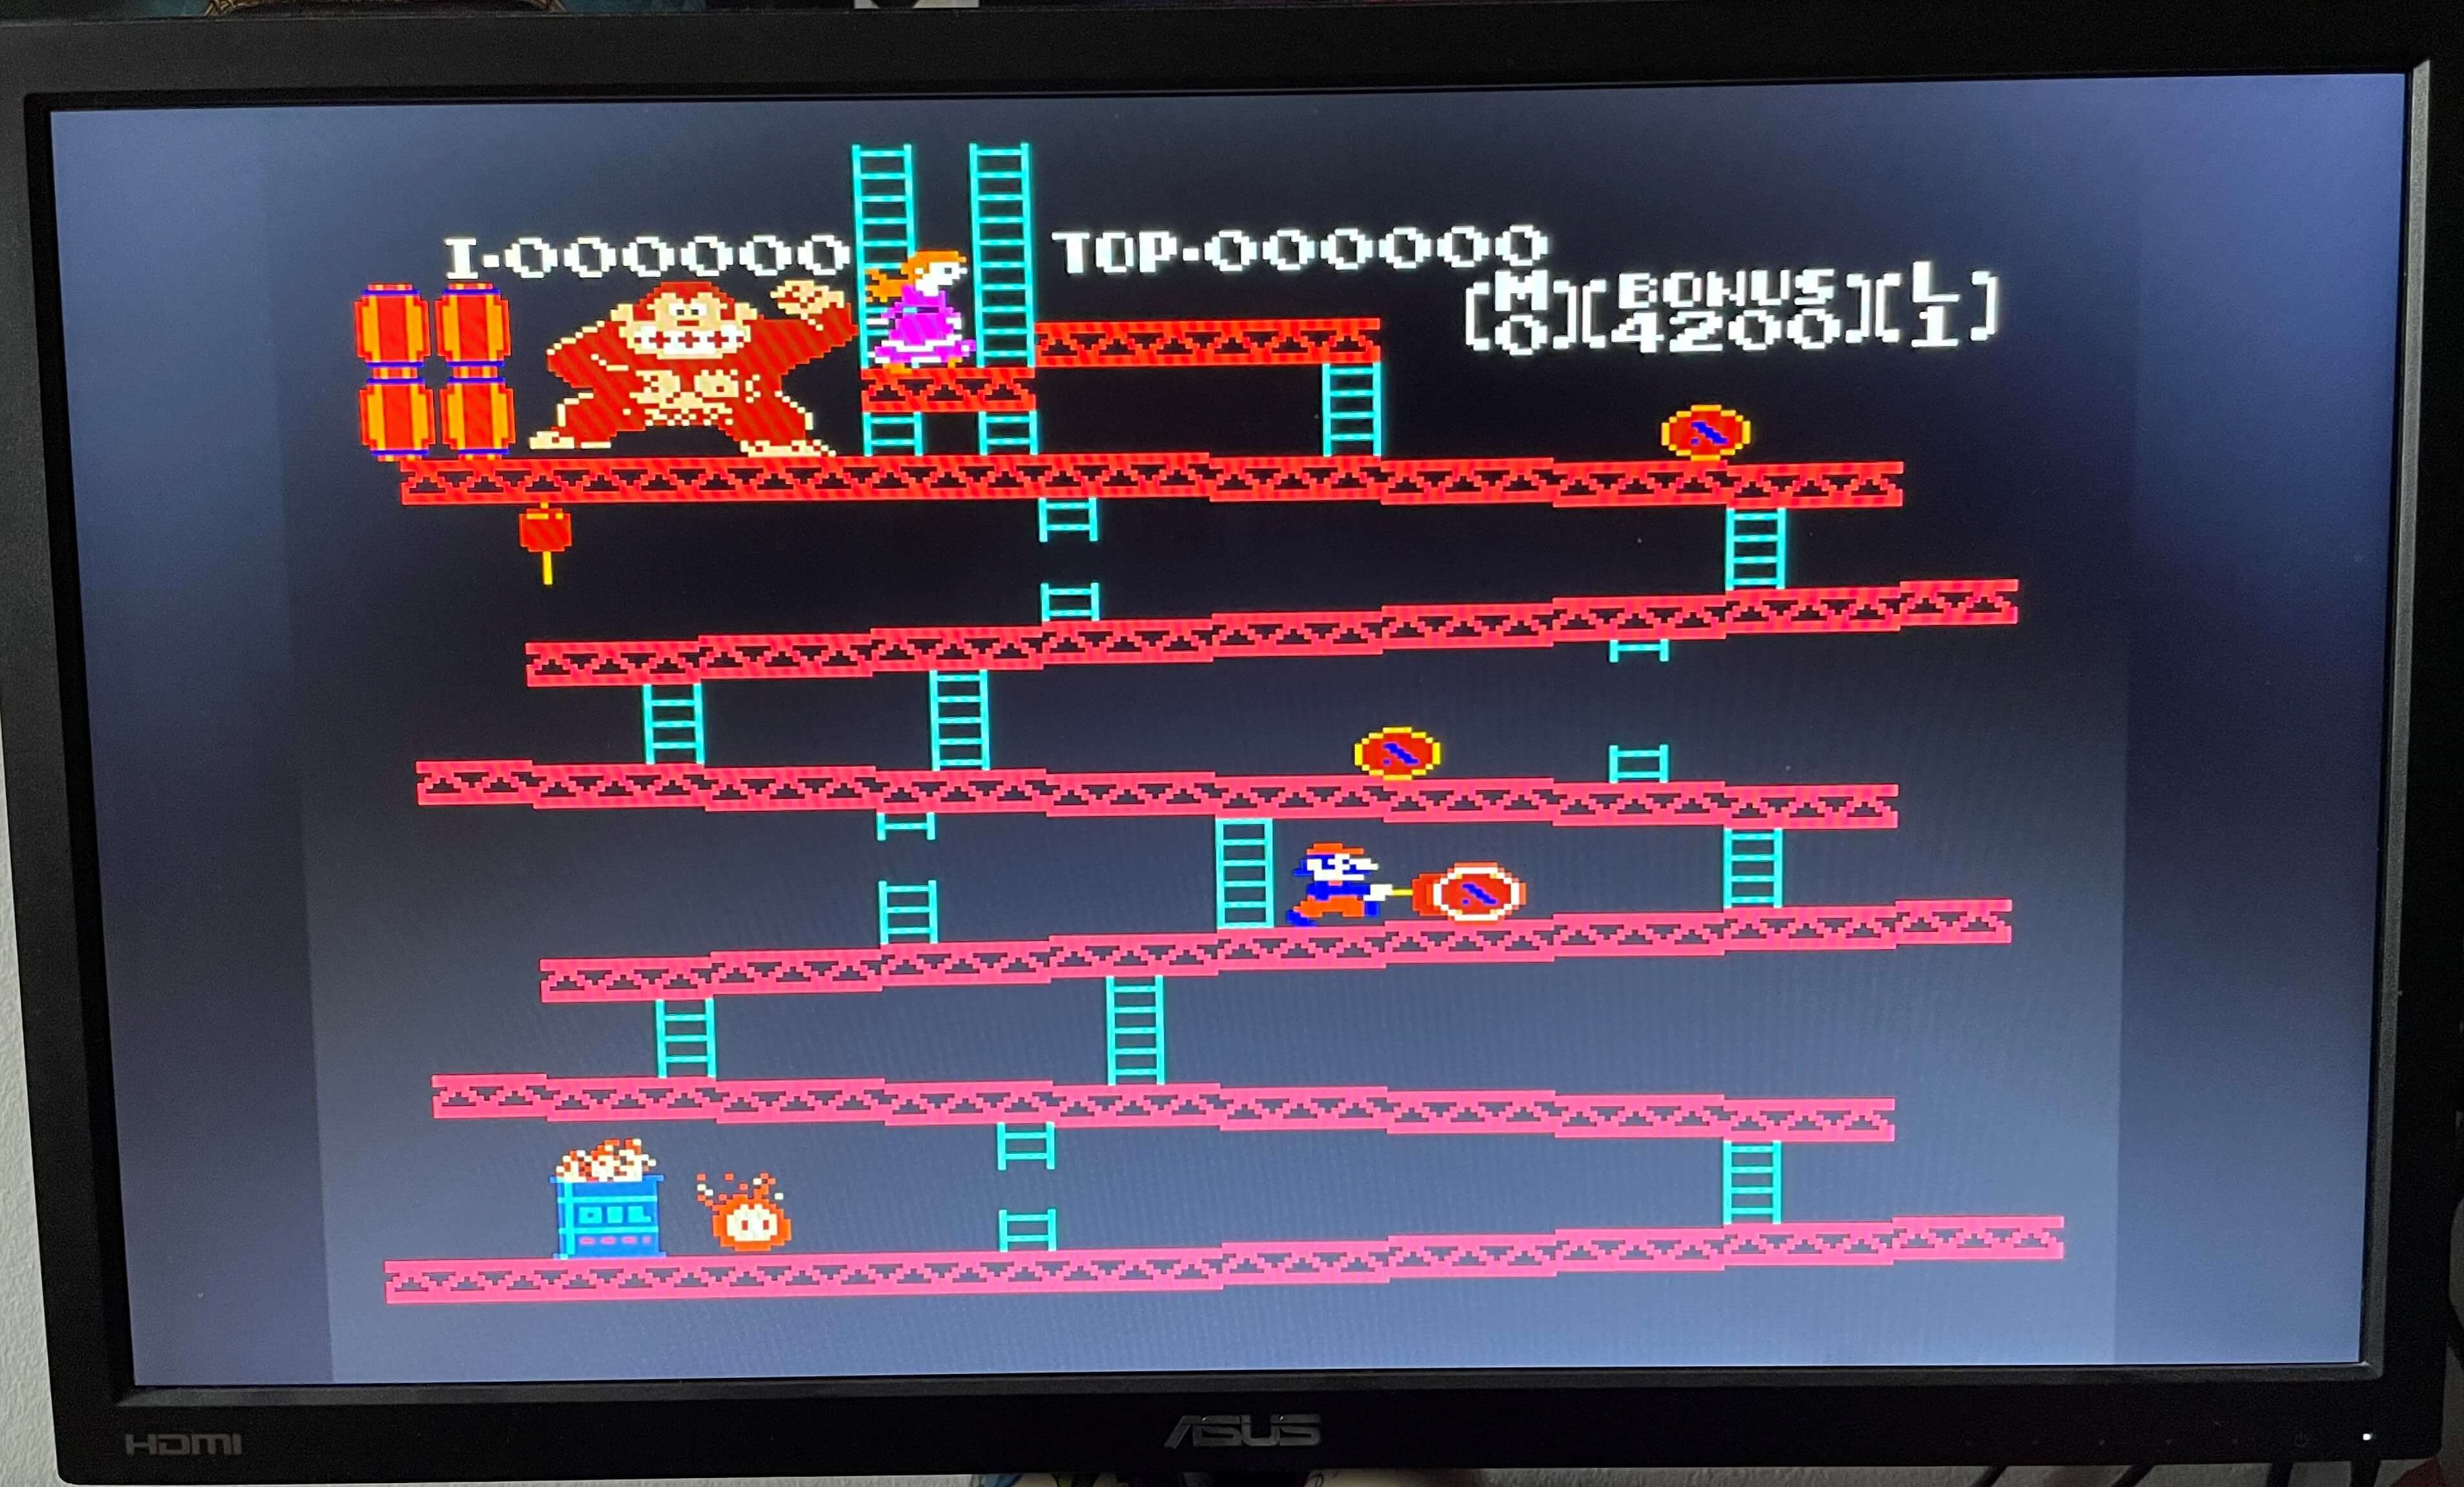
\includegraphics[width=150mm, keepaspectratio]{figures/Donkey-level-1}
	\caption{Donkey Kong ikonikus első pálya futás közben} 
	\label{fig:Donkey-level-1}
\end{figure}

\begin{figure}[H]
	\centering
	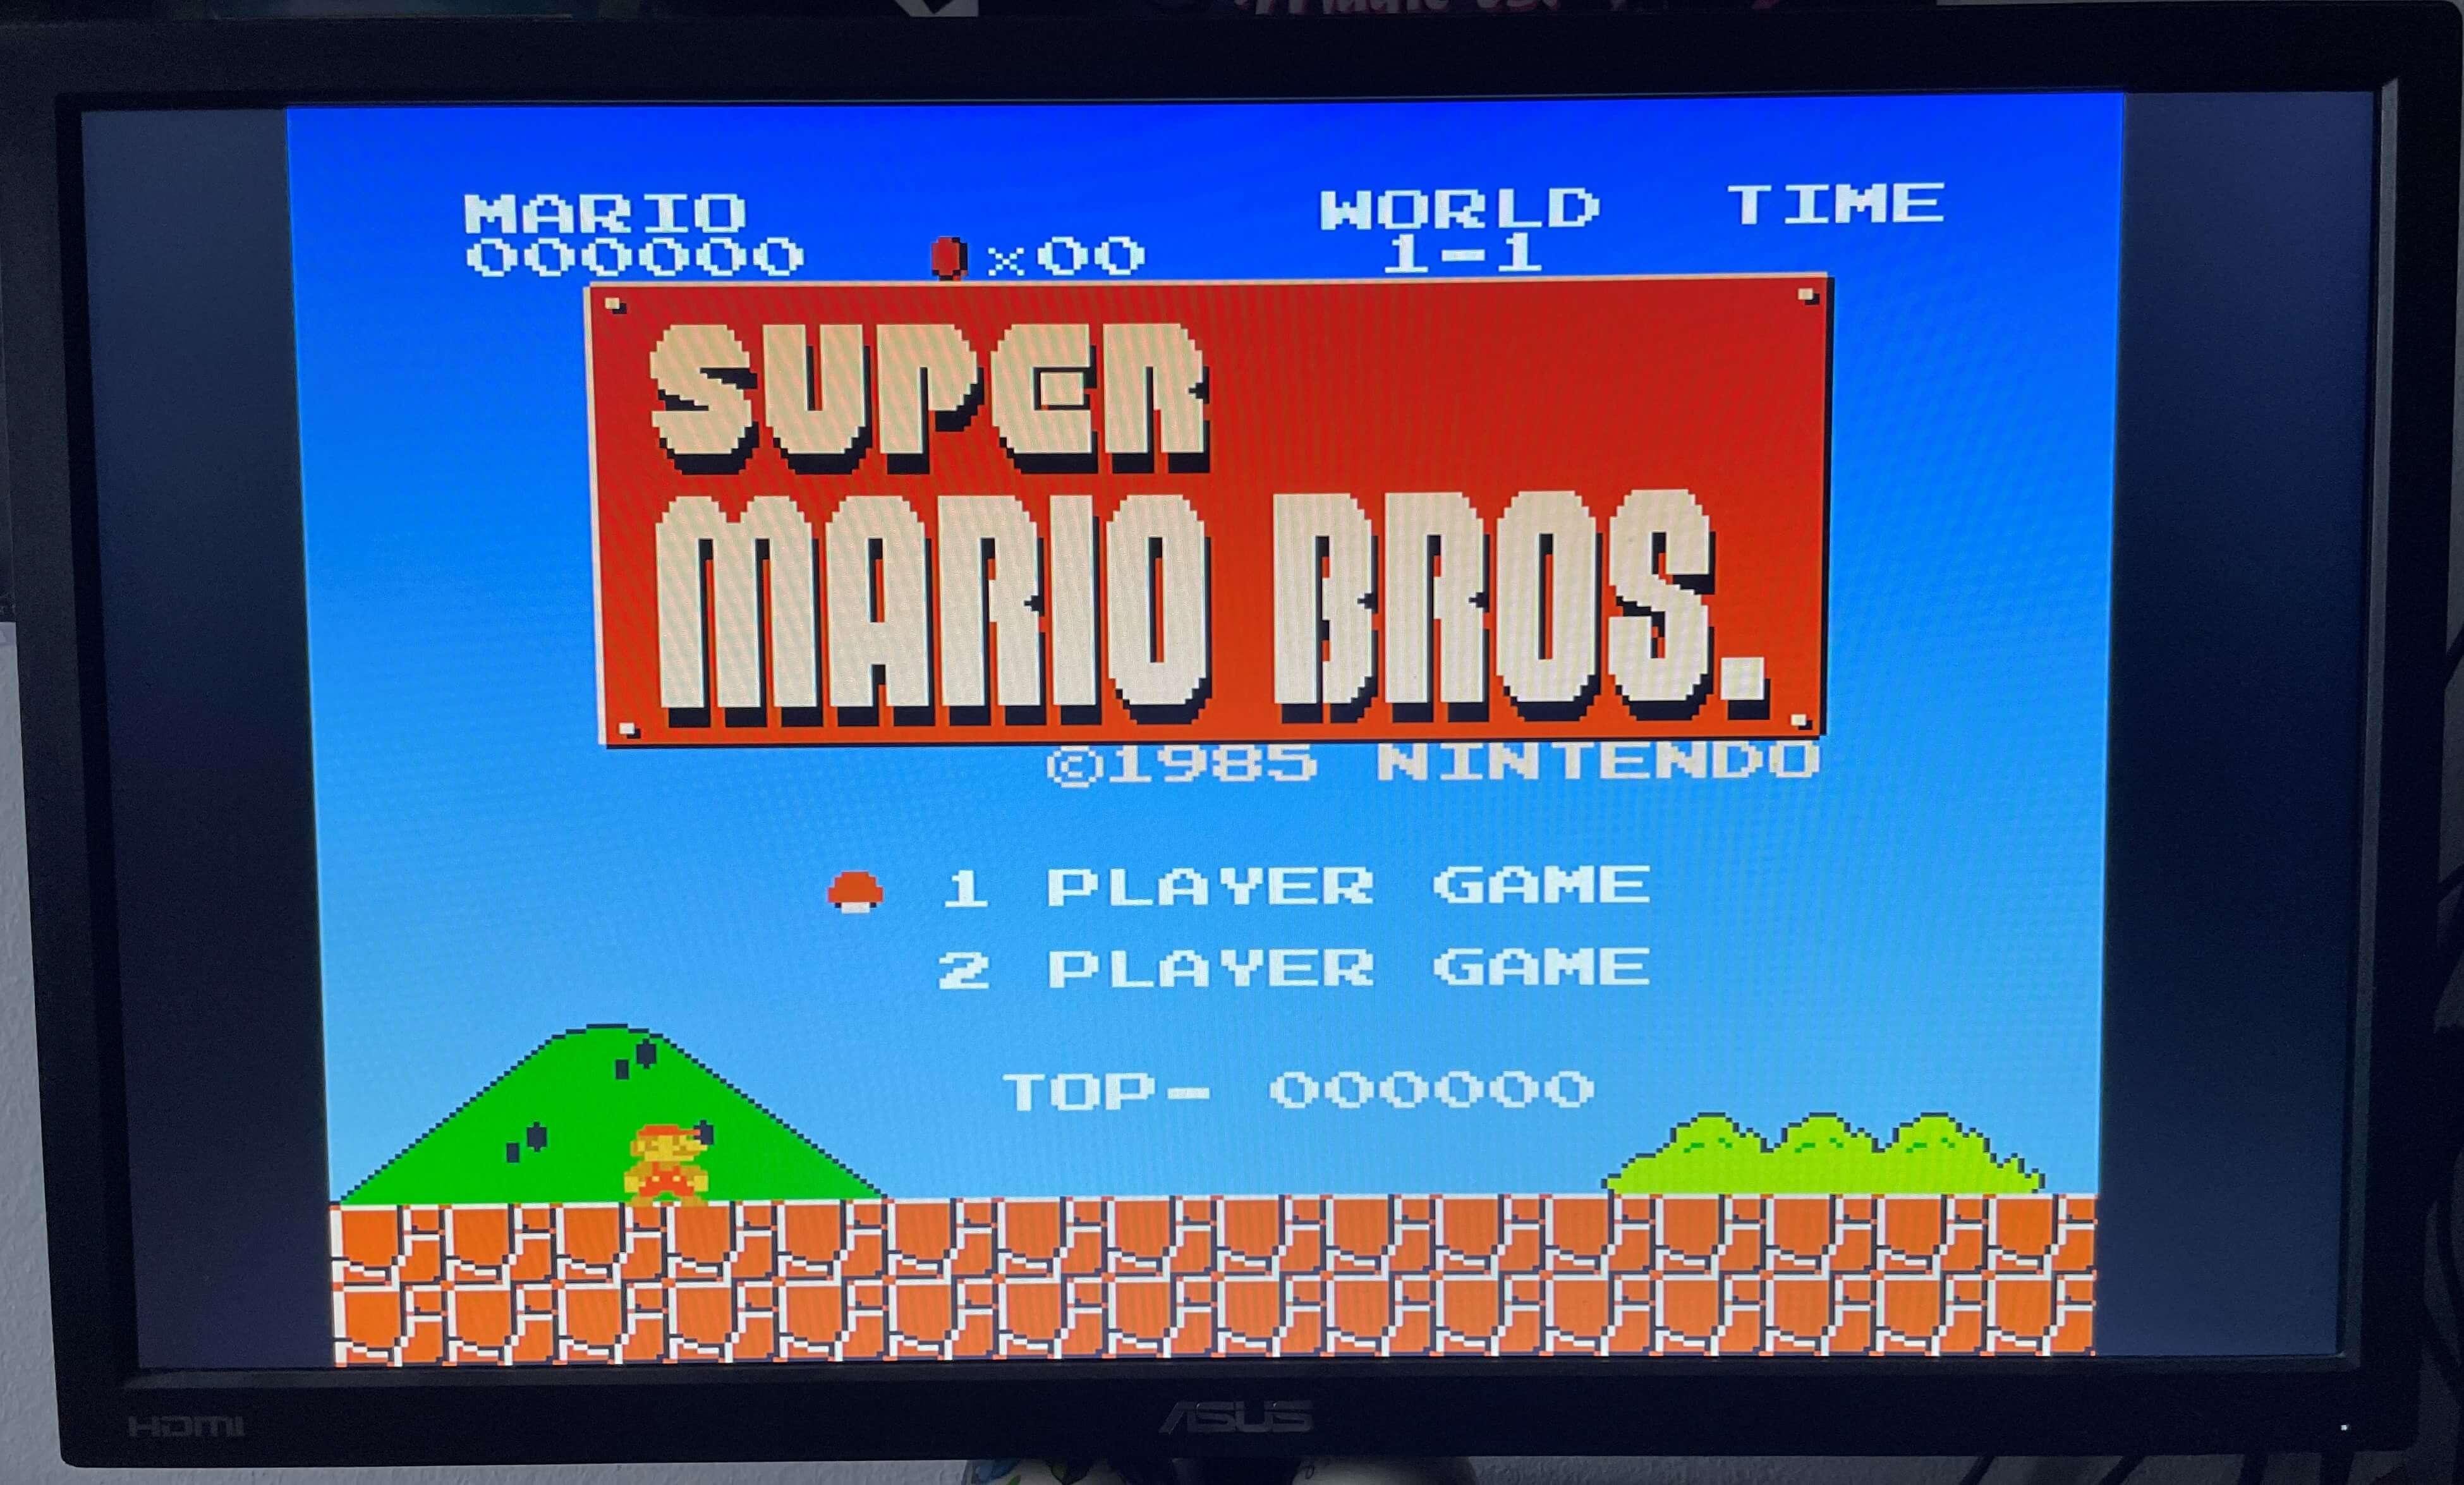
\includegraphics[width=150mm, keepaspectratio]{figures/Super-Mario_Start-croped}
	\caption{A Super Mario Bros. kezdő képernyője} 
	\label{fig:Super-Mario-start}
\end{figure}

\begin{figure}[H]
	\centering
	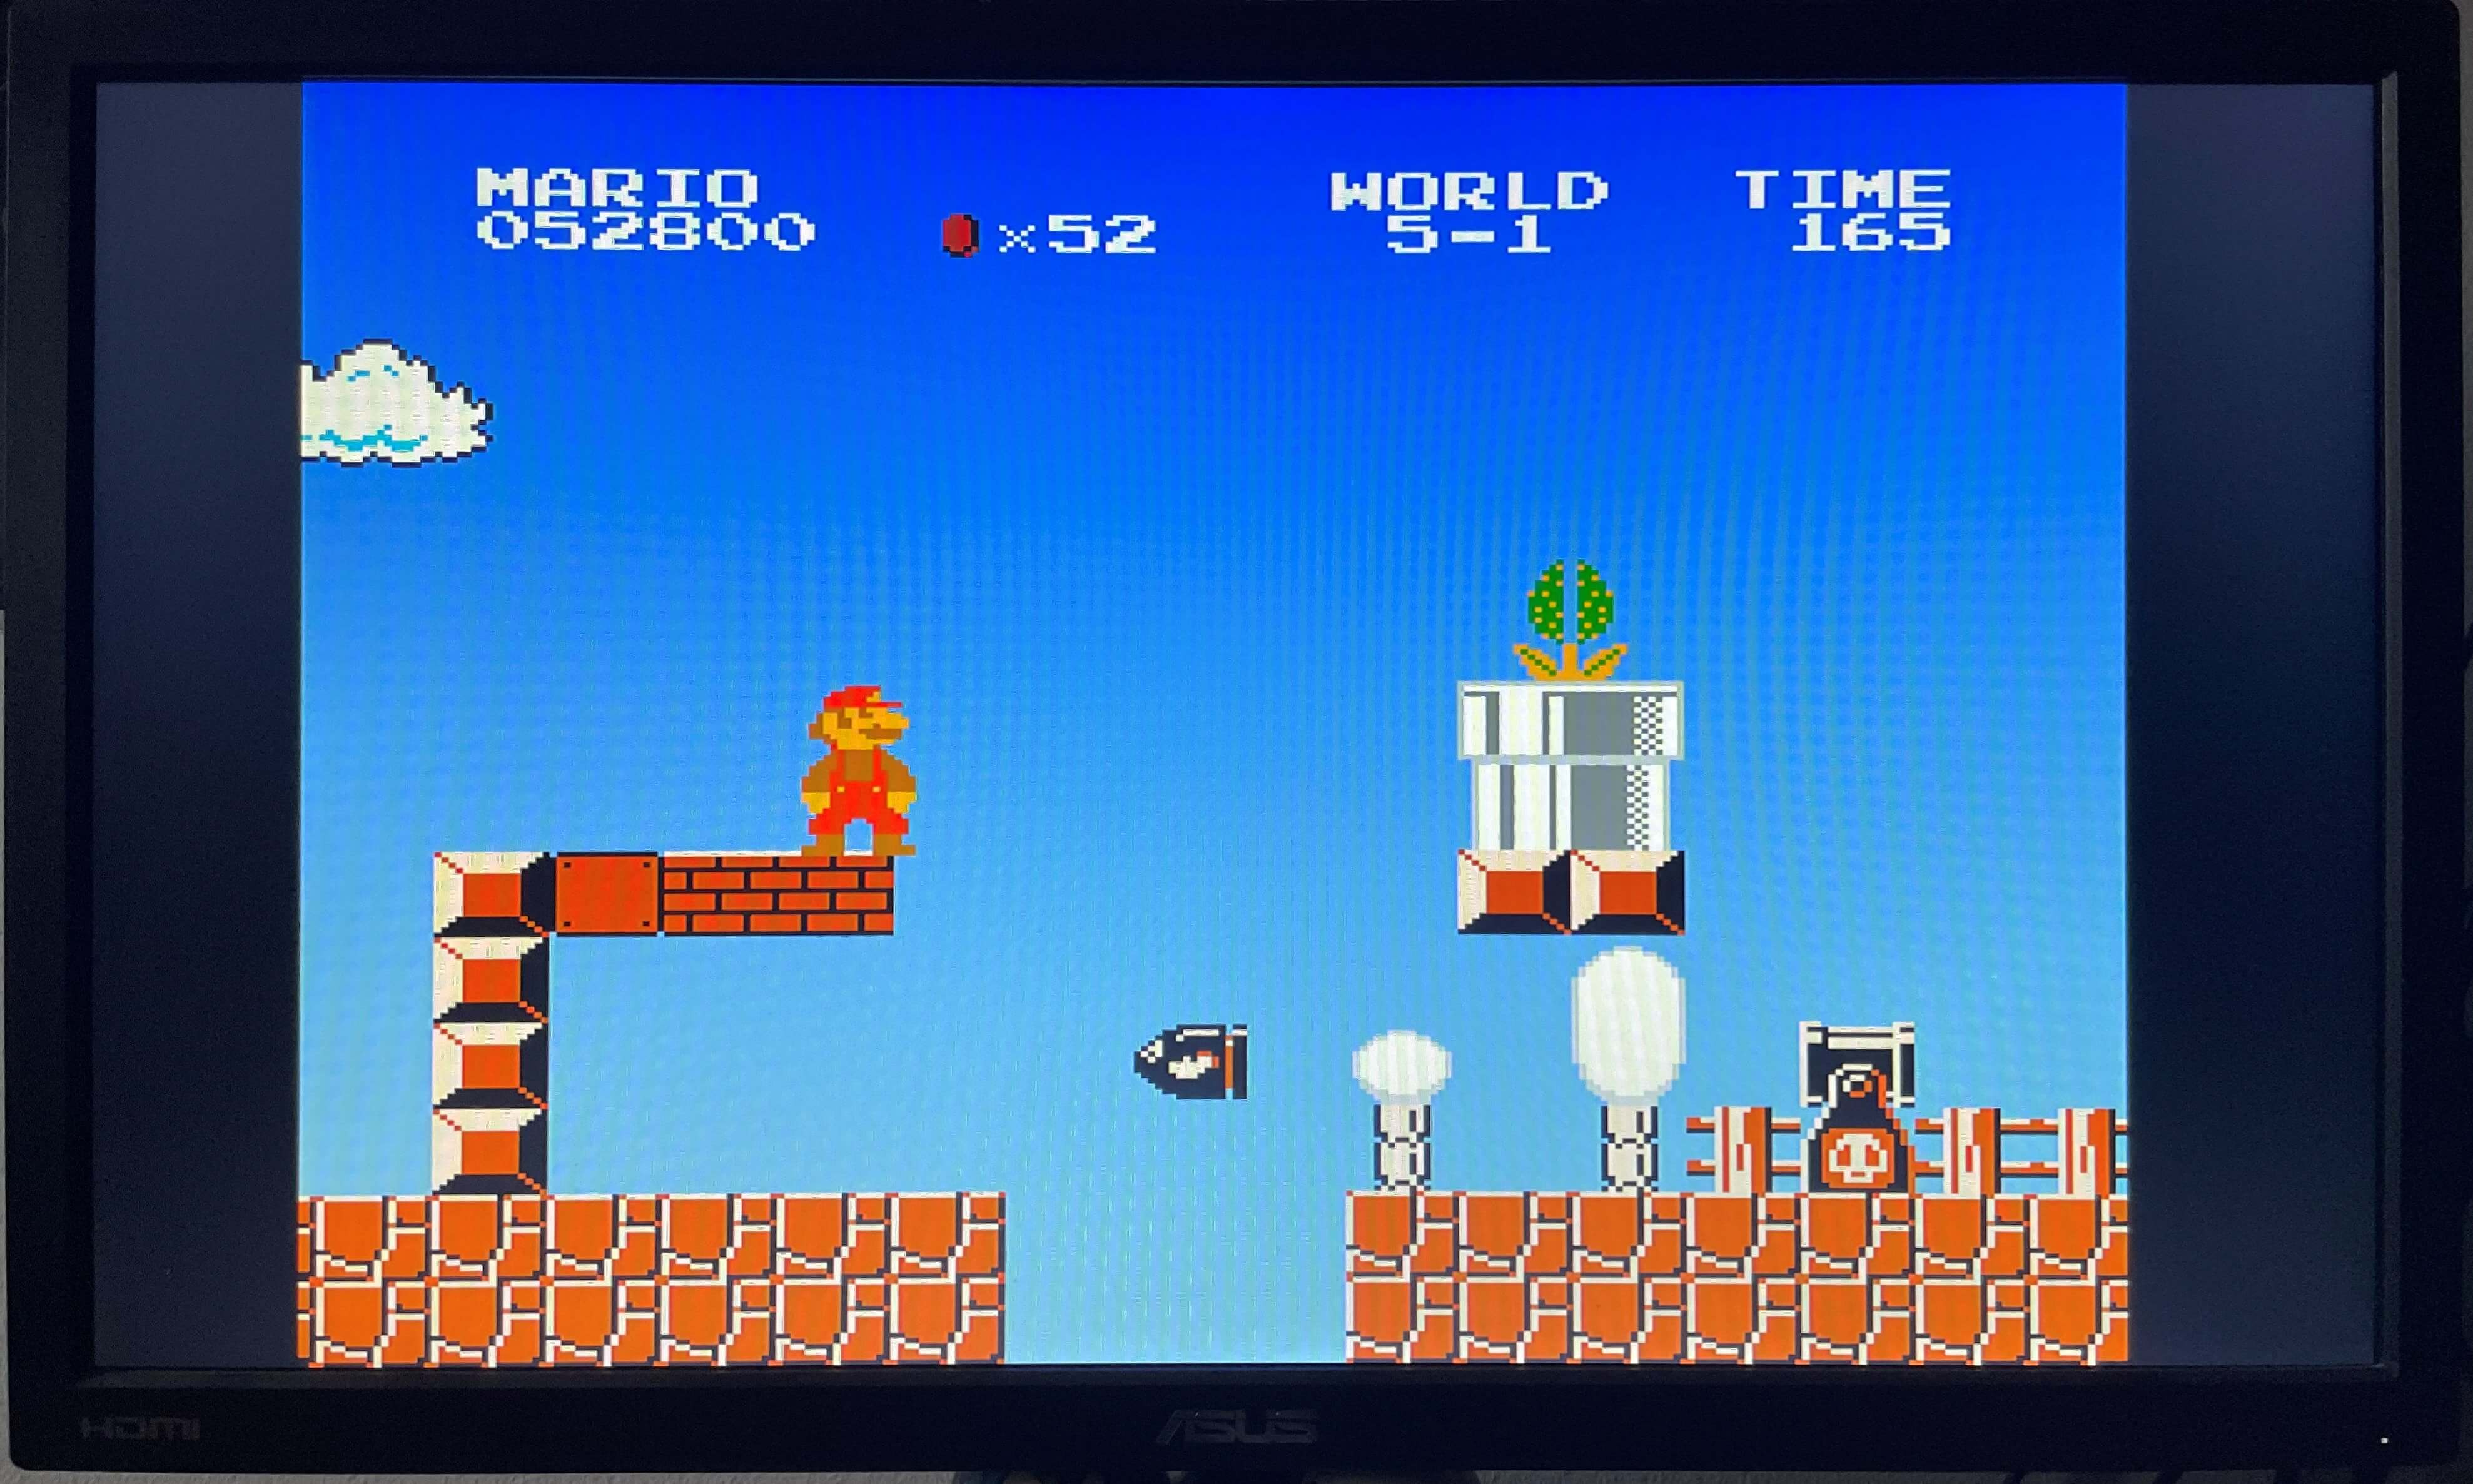
\includegraphics[width=150mm, keepaspectratio]{figures/Super-Mario-world5-1-croped}
	\caption{A Super Mario Bros. ötödik világának első pályája} 
	\label{fig:Super-Mario-world5-1}
\end{figure}

\section{A tesztek eredményeinek kiértékelése}

A szimulációs tesztek során sikeresen fel tudtam éleszteni a NES rendszerét olyan szintre, hogy elkezdhettem a hardveres teszteket. A későbbiek során is voltak olyan hardveres modulok, amelyekben hibakeresés során többször is visszanyúltam a szimulátorhoz. Sajnos a ISim hibás működése miatt a teljes rendszert nem tudtam nyomon követni, viszont a szimulációk során megfigyelt hardveres működéseket \aref{sec:fpga-desing-begining}. fejezetben több helyen is láthatjuk.

A hardveres tesztelések eredménye is sikeres lett, a két játék teljes mértékben játszható állapotban van. A hosszabb tesztelések során sem akadtam olyan hibára, amely a programok futását megakadályoznák és ezzel a játékokat játszhatatlanná tennék. A képalkotásért felelős chip a PPU időzítései is pontosak, hiszen még az idő kritikus játékok, mint a Mario is játszható a konzolon. Ez \aref{fig:Super-Mario-world5-1}. ábrán is látható. Itt még jól megfigyelhető az is, hogy a PPU háttér és sprite alkotási része is összhangban van (egy sűrűbb mozgó elemekkel teli képen sem hibásodik meg a képalkotás). Az általam használt színpaletták, szépen visszaadják az eredeti NES játékok színvilágát, ezzel egy nagyon jó minőségű emulálást lehetővé téve.

Úgy érzem az FPGA-s hardverfejlesztések teszteléseinek széleskörű tárházát ismertem meg, és ezen eszközök segítségével sikeresen működésre bírtam az általam fejlesztett konzol hardverét.
\chapter{Összefoglalás, jövőbeli tervek}

A Diplomatervezés 1 során sikerült foglalkoznom a projekt irodalom kutatásával, és NES nyomtatott áramkörének FPGA alapú újratervezésével, illetve a PPU hardverének felépítésével és felújításával.

A Diplomatervezés végeztéig még meg kell ismernem a CPU és APU hardverét is részletesen, illetve ezeket a PPU-val együtt meg kell terveznem a spatan-6-os FPGA-ba. Ezt követően pedig tesztelnem kell ezeket az éles hardveren.

A projekt hosszútávú tervei közé tartozik az MicroSD kártyáról történő játék betöltés és minél több NES játék mapper-ének lefejlesztése, ezzel teljes körű hardveres emulálást készítve a Nintendo Entertainment System-hez. 


% Acknowledgements
%~~~~~~~~~~~~~~~~~~~~~~~~~~~~~~~~~~~~~~~~~~~~~~~~~~~~~~~~~~~~~~~~~~~~~~~~~~~~~~~~~~~~~~
%----------------------------------------------------------------------------
\chapter*{\koszonetnyilvanitas}\addcontentsline{toc}{chapter}{\koszonetnyilvanitas}
%----------------------------------------------------------------------------

A diplomaterv készítése során nagyban támaszkodhattam mind a tanszéki konzulensem Raikovich  Tamás, mind a NESDev wiki közösség tanácsaira. Köszönettel tartozom a konzulensemnek a támogatásáért, ötleteiért és azért, mert az ő processzora nélkül nem jutott volna el ilyen szintre a projekt. Úgy érzem, hogy nekik köszönhetően tudtam a tőlem telhető maximumot megtenni a diplomaterv projekt elkészítése során.


% List of Figures, Tables
%~~~~~~~~~~~~~~~~~~~~~~~~~~~~~~~~~~~~~~~~~~~~~~~~~~~~~~~~~~~~~~~~~~~~~~~~~~~~~~~~~~~~~~
%\listoffigures\addcontentsline{toc}{chapter}{\listfigurename}
%\listoftables\addcontentsline{toc}{chapter}{\listtablename}


% Bibliography
%~~~~~~~~~~~~~~~~~~~~~~~~~~~~~~~~~~~~~~~~~~~~~~~~~~~~~~~~~~~~~~~~~~~~~~~~~~~~~~~~~~~~~~
\addcontentsline{toc}{chapter}{\bibname}
\bibliography{bib/mybib}


% Appendix
%~~~~~~~~~~~~~~~~~~~~~~~~~~~~~~~~~~~~~~~~~~~~~~~~~~~~~~~~~~~~~~~~~~~~~~~~~~~~~~~~~~~~~~
%----------------------------------------------------------------------------
\appendix
%----------------------------------------------------------------------------
\chapter*{\fuggelek}\addcontentsline{toc}{chapter}{\fuggelek}
\setcounter{chapter}{\appendixnumber}
%\setcounter{equation}{0} % a fofejezet-szamlalo az angol ABC 6. betuje (F) lesz
\numberwithin{equation}{section}
\numberwithin{figure}{section}
\numberwithin{lstlisting}{section}
%\numberwithin{tabular}{section}

%TODO new fugellek here
\newpage
\section{FPGA NES kártya kapcsolási rajza}
\subsection{Tápegység}
\begin{figure}[H]
	\centering
	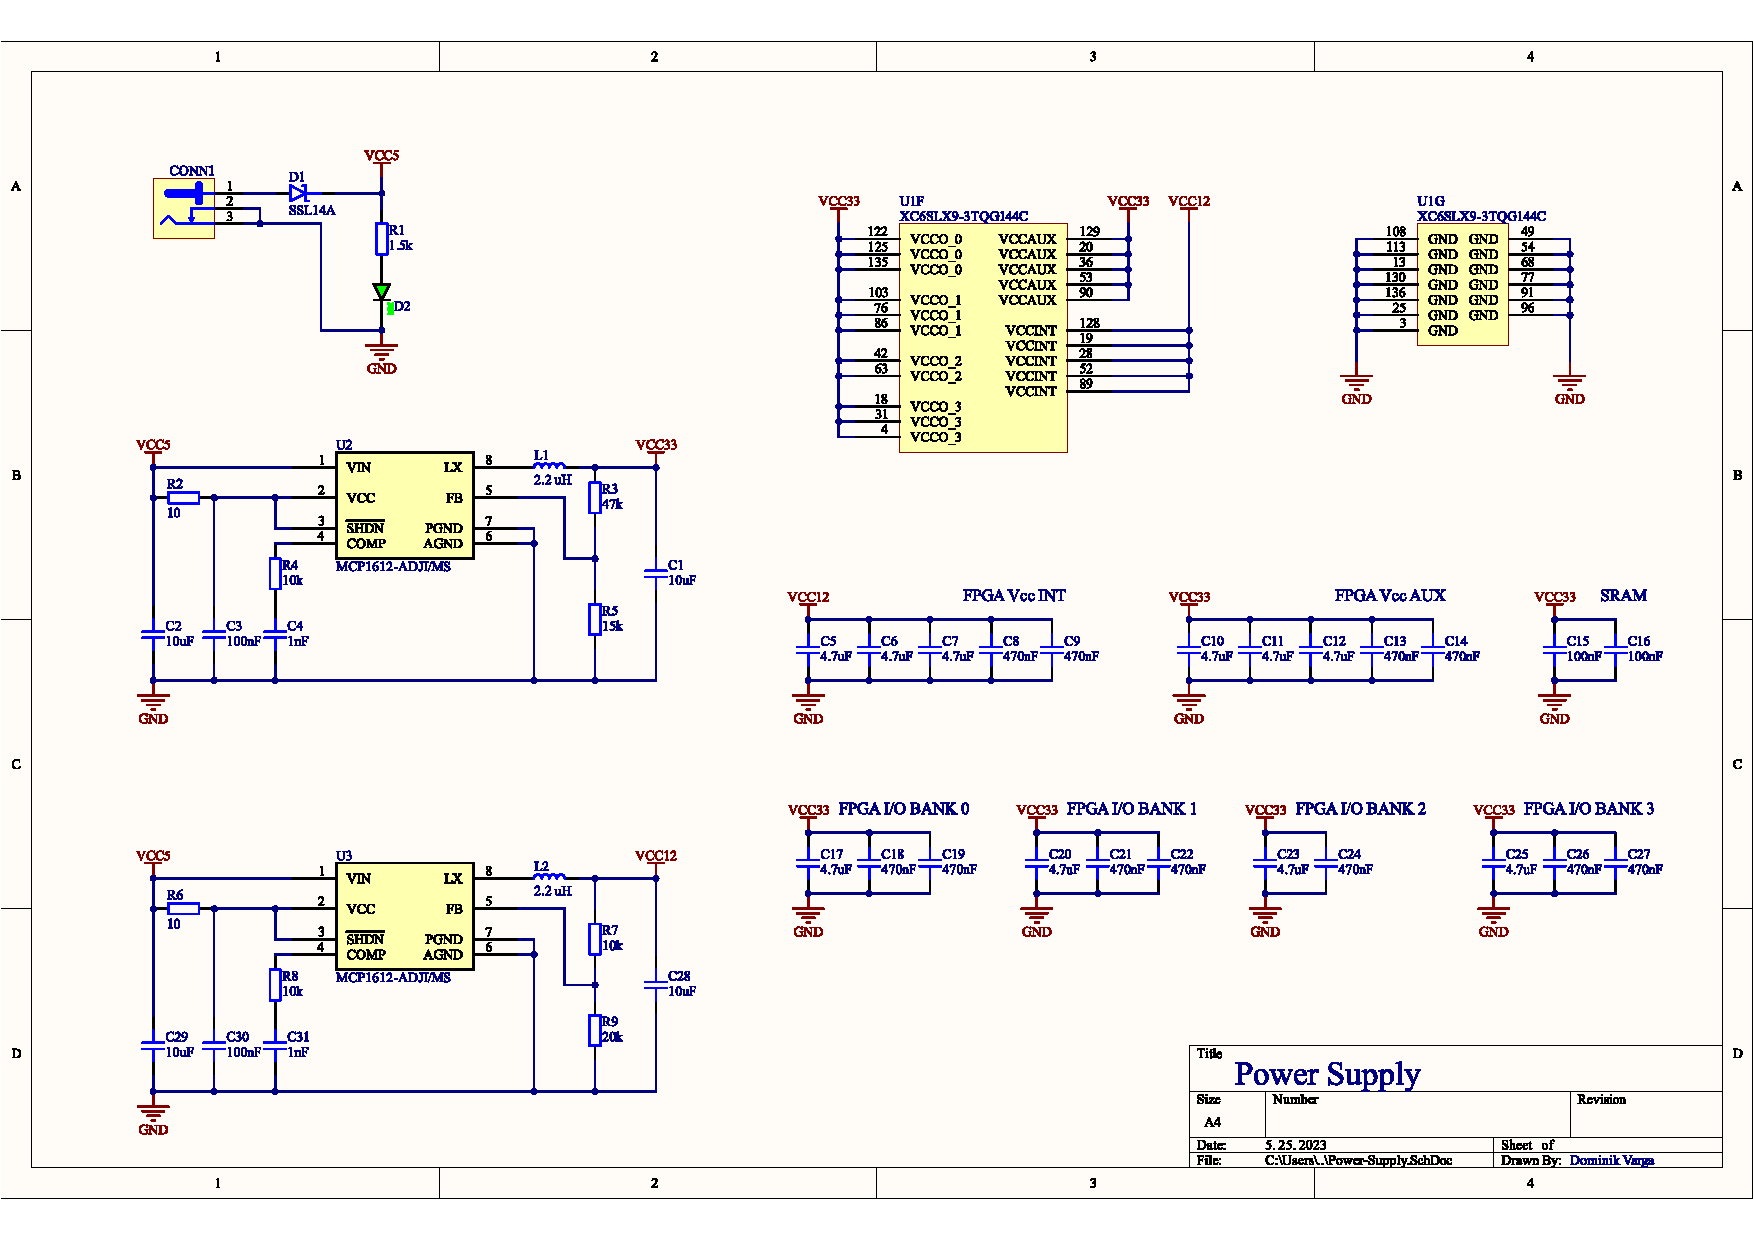
\includegraphics[width=220mm, keepaspectratio, angle=90]{figures/PSU}
	%\caption{Tápegység} 
	\label{fig:PSU}
\end{figure}
\subsection{HDMI és MicroSD kártya csatlakozó}
\begin{figure}[H]
	\centering
	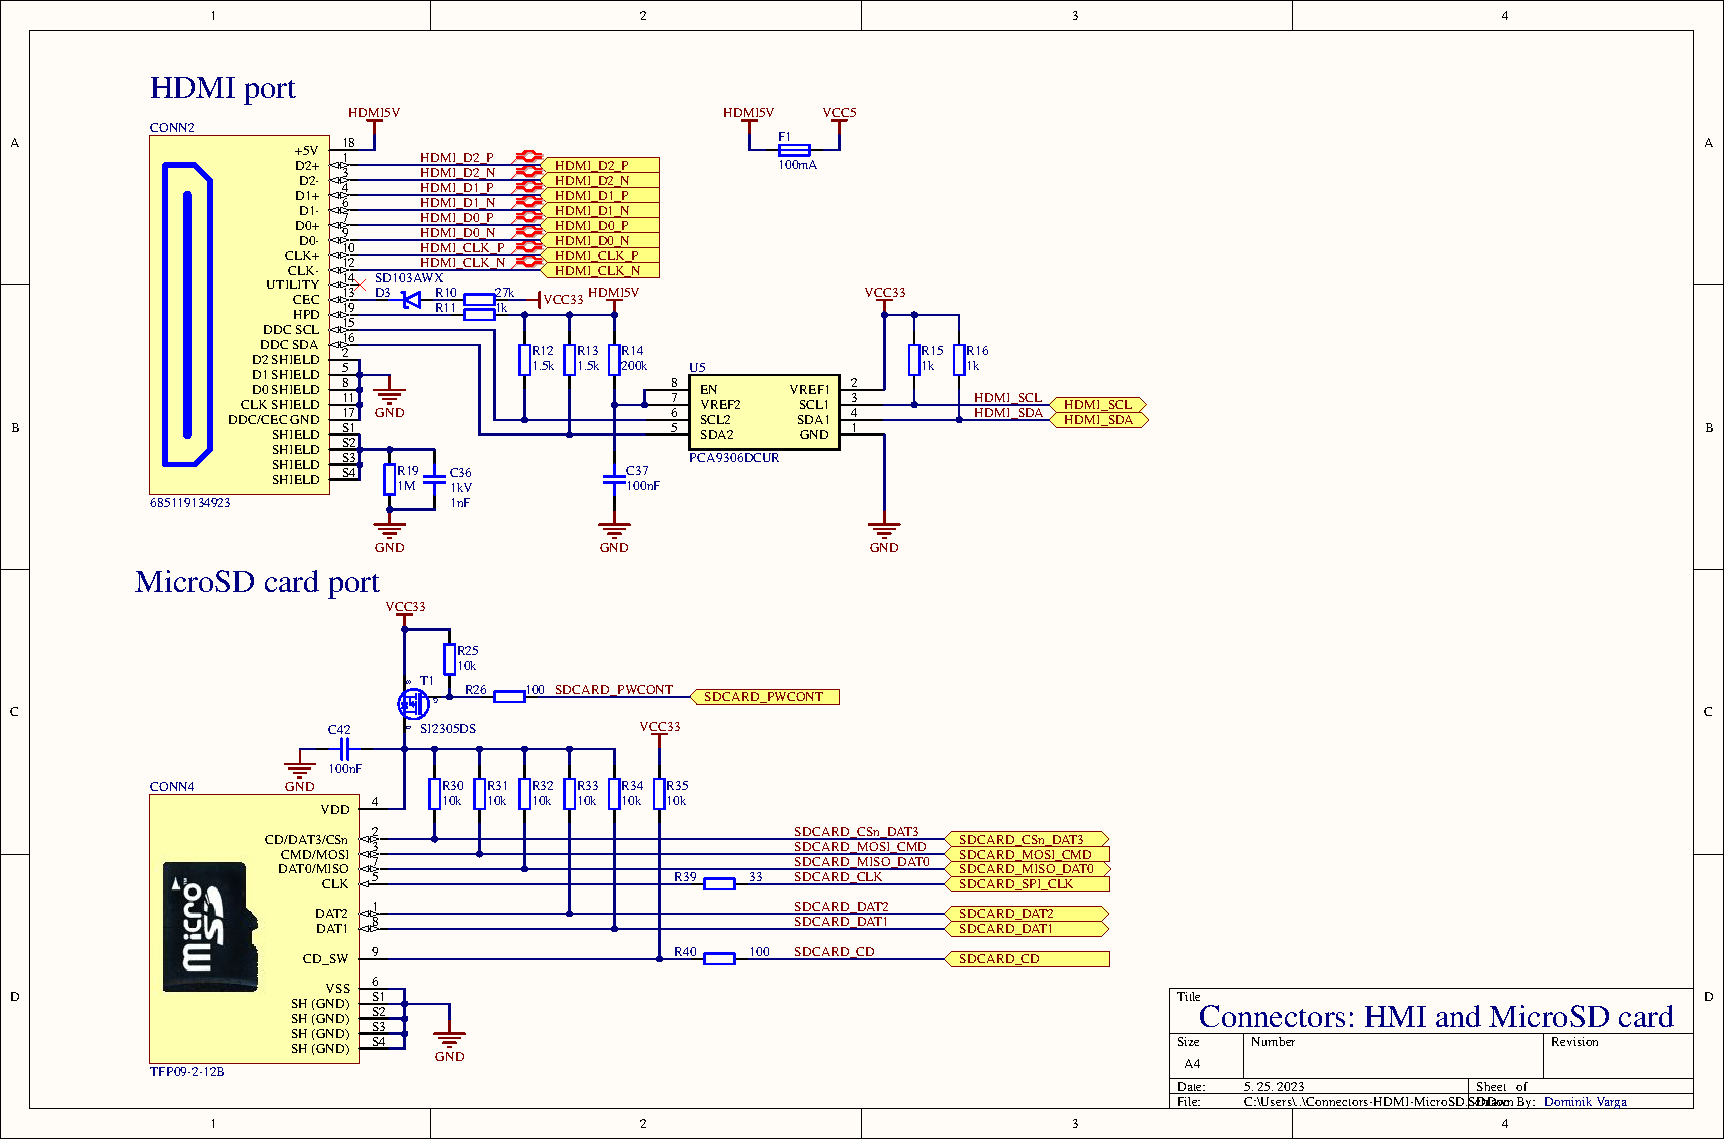
\includegraphics[width=220mm, keepaspectratio, angle=90]{figures/HDMI-MicroSDcard}
	%\caption{HDMI és MicroSD kártya csatlakozó} 
	\label{fig:HDMI-MicroSDcard}
\end{figure}
\subsection{DAC, erősítő és kontroller áramkörök}
\begin{figure}[H]
	\centering
	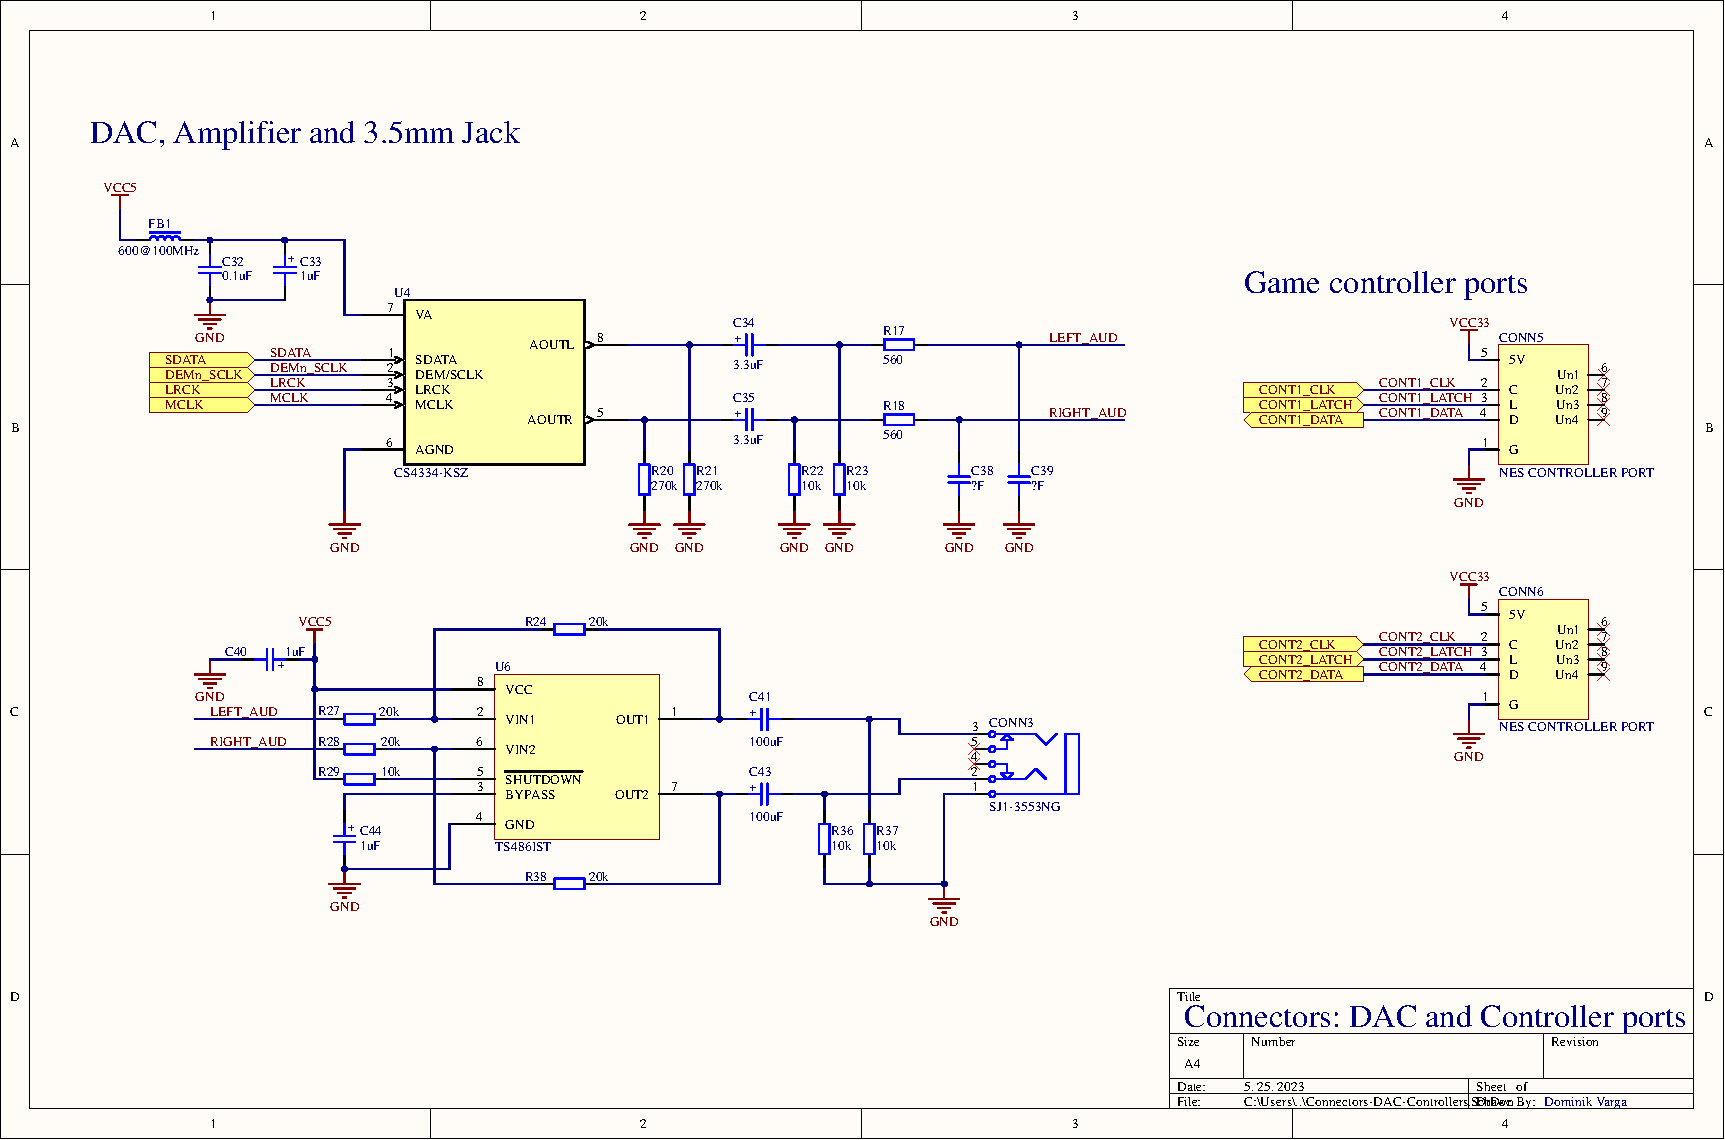
\includegraphics[width=220mm, keepaspectratio, angle=90]{figures/DAC-CONTROLLER}
	%\caption{DAC, erősítő és kontroller áramkörök} 
	\label{fig:DAC-controllers}
\end{figure}
\subsection{SRAM és SPI-Flash}
\begin{figure}[H]
	\centering
	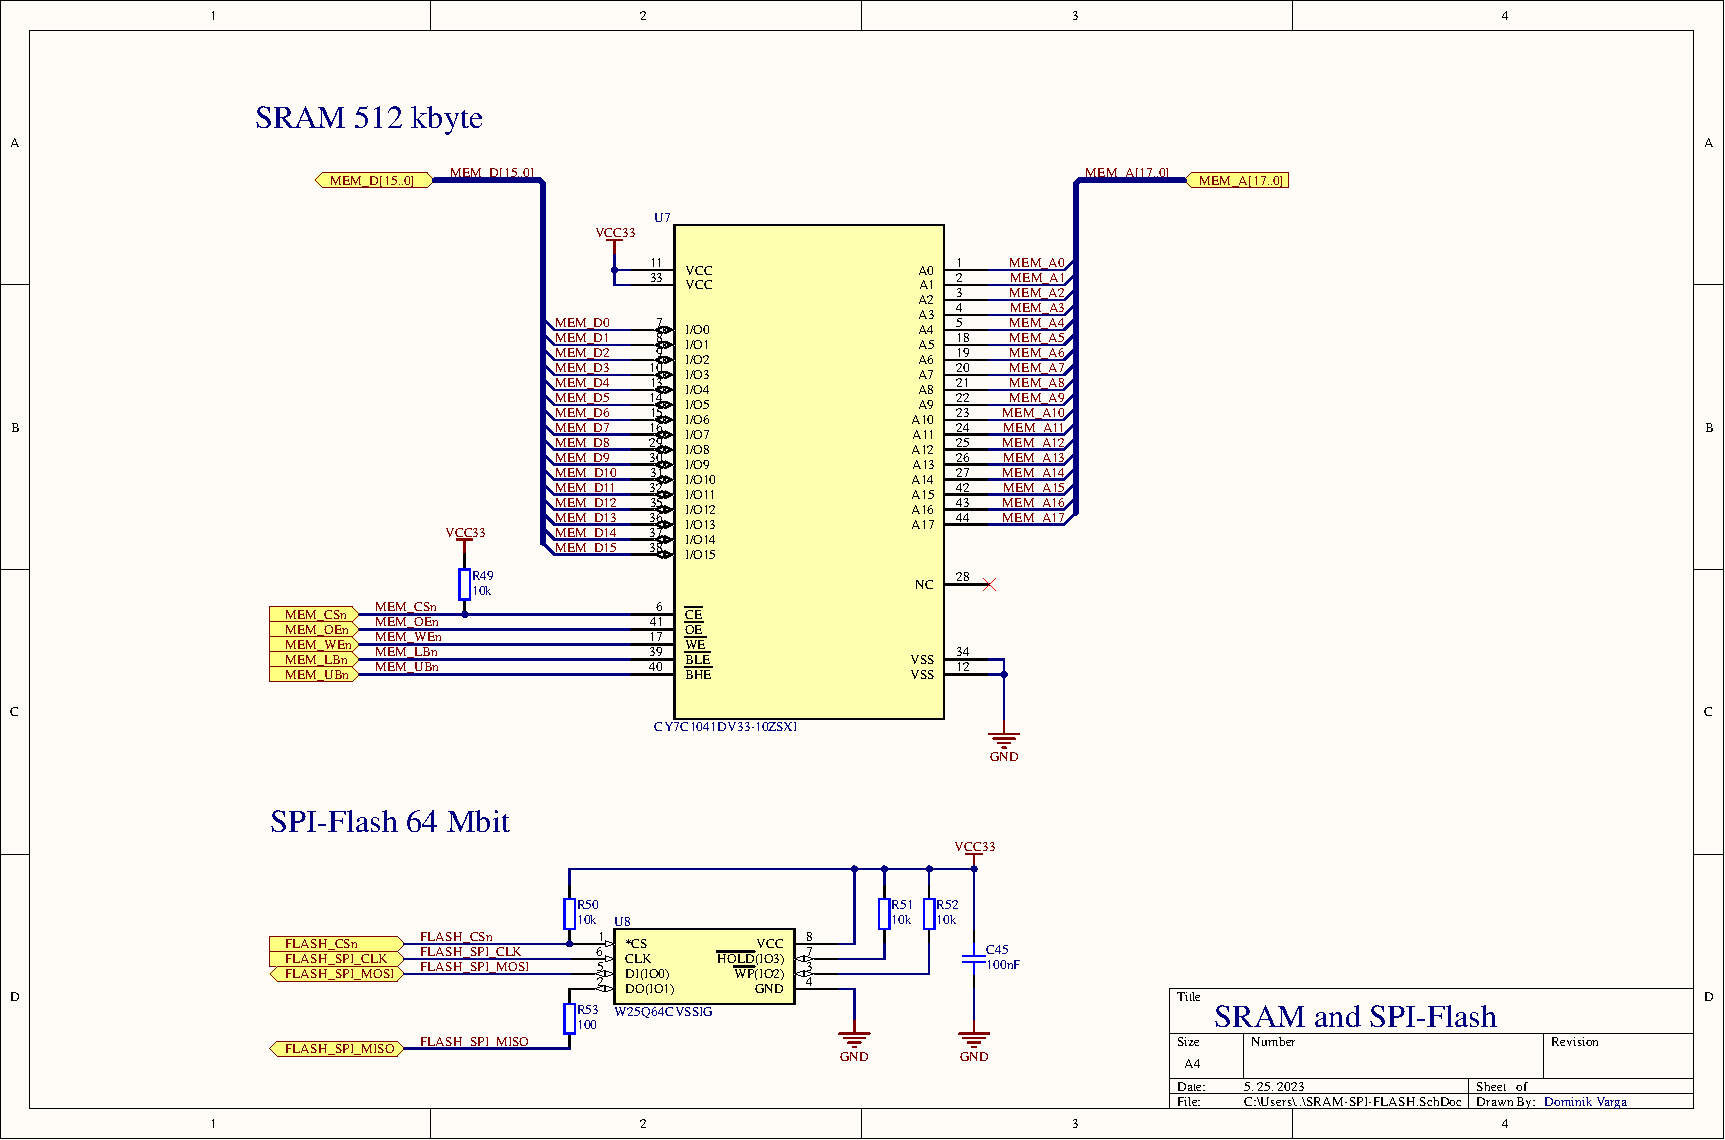
\includegraphics[width=220mm, keepaspectratio, angle=90]{figures/SRAM-FLASH}
	%\caption{SRAM és SPI-Flash} 
	\label{fig:SRAM-SPI-Flash}
\end{figure}
\subsection{FPGA OSC és JTAG}
\begin{figure}[H]
	\centering
	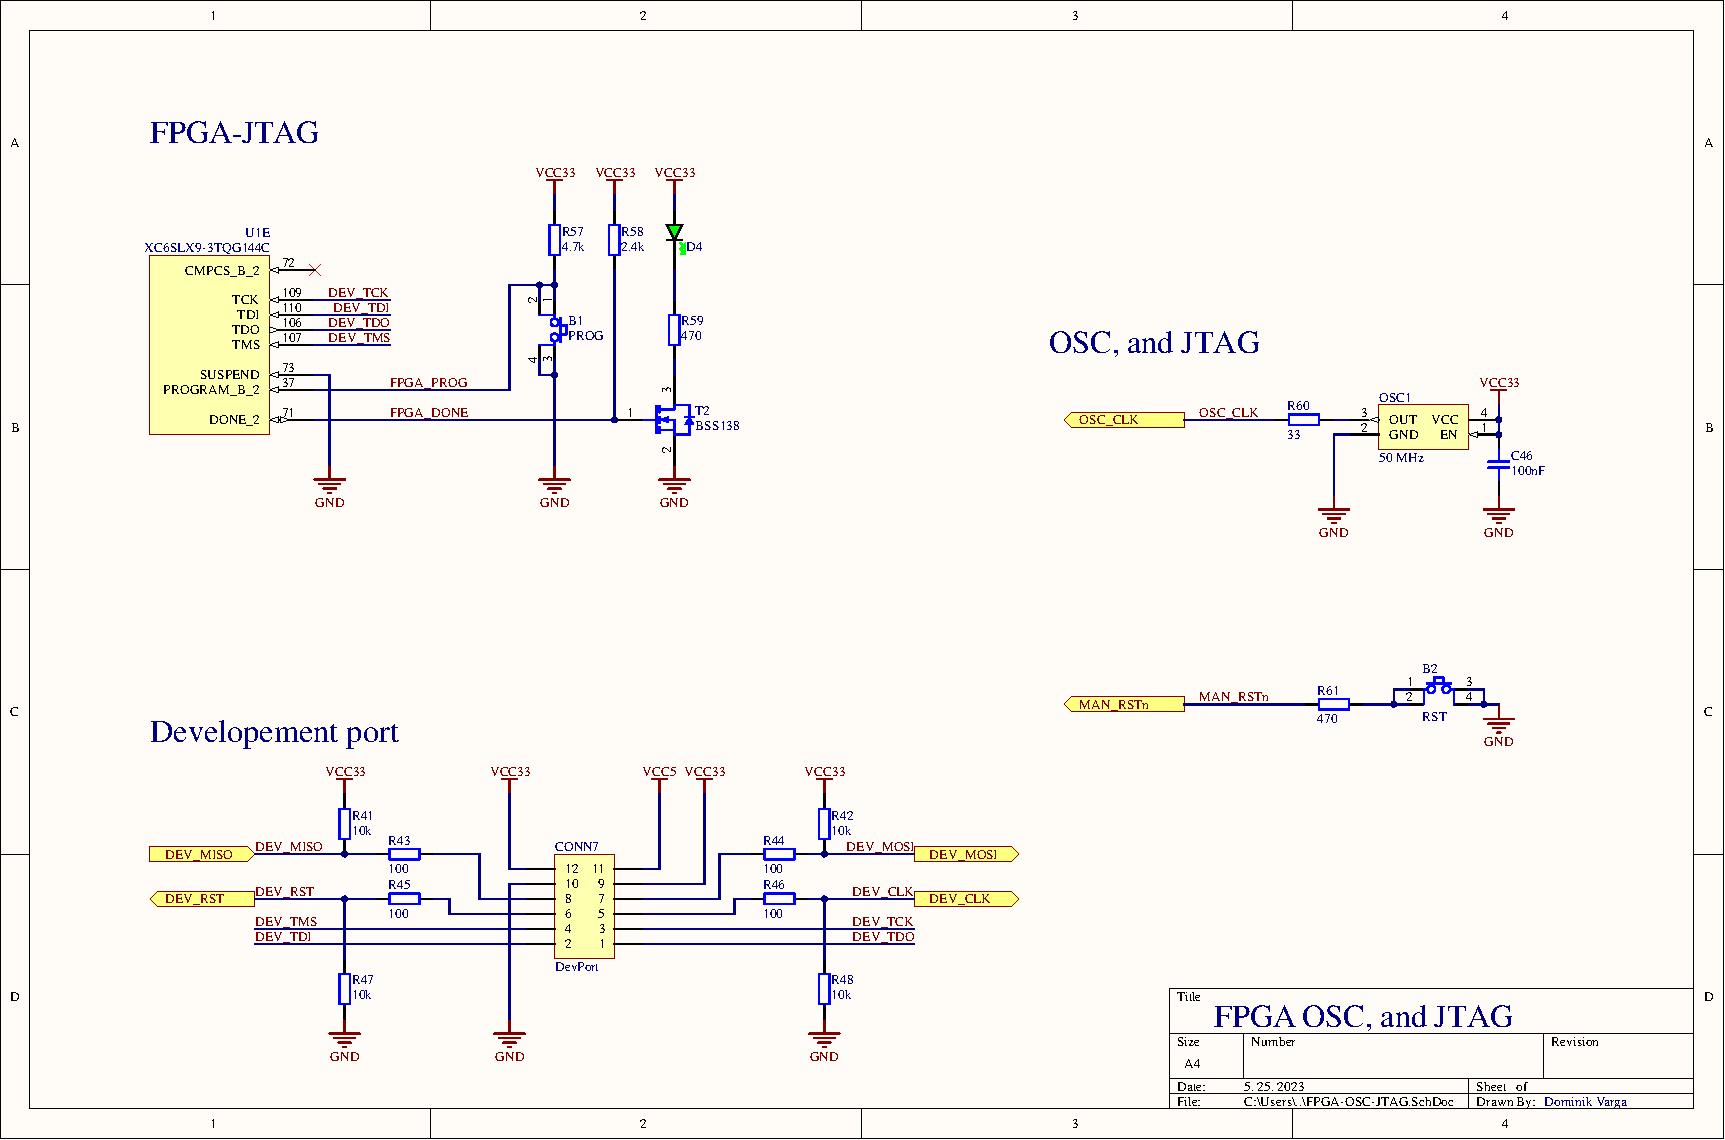
\includegraphics[width=220mm, keepaspectratio, angle=90]{figures/JTAG-OSC}
	%\caption{FPGA OSC és JTAG} 
	\label{fig:OSC-JTAG}
\end{figure}
\subsection{FPGA IO bankok}
\begin{figure}[H]
	\centering
	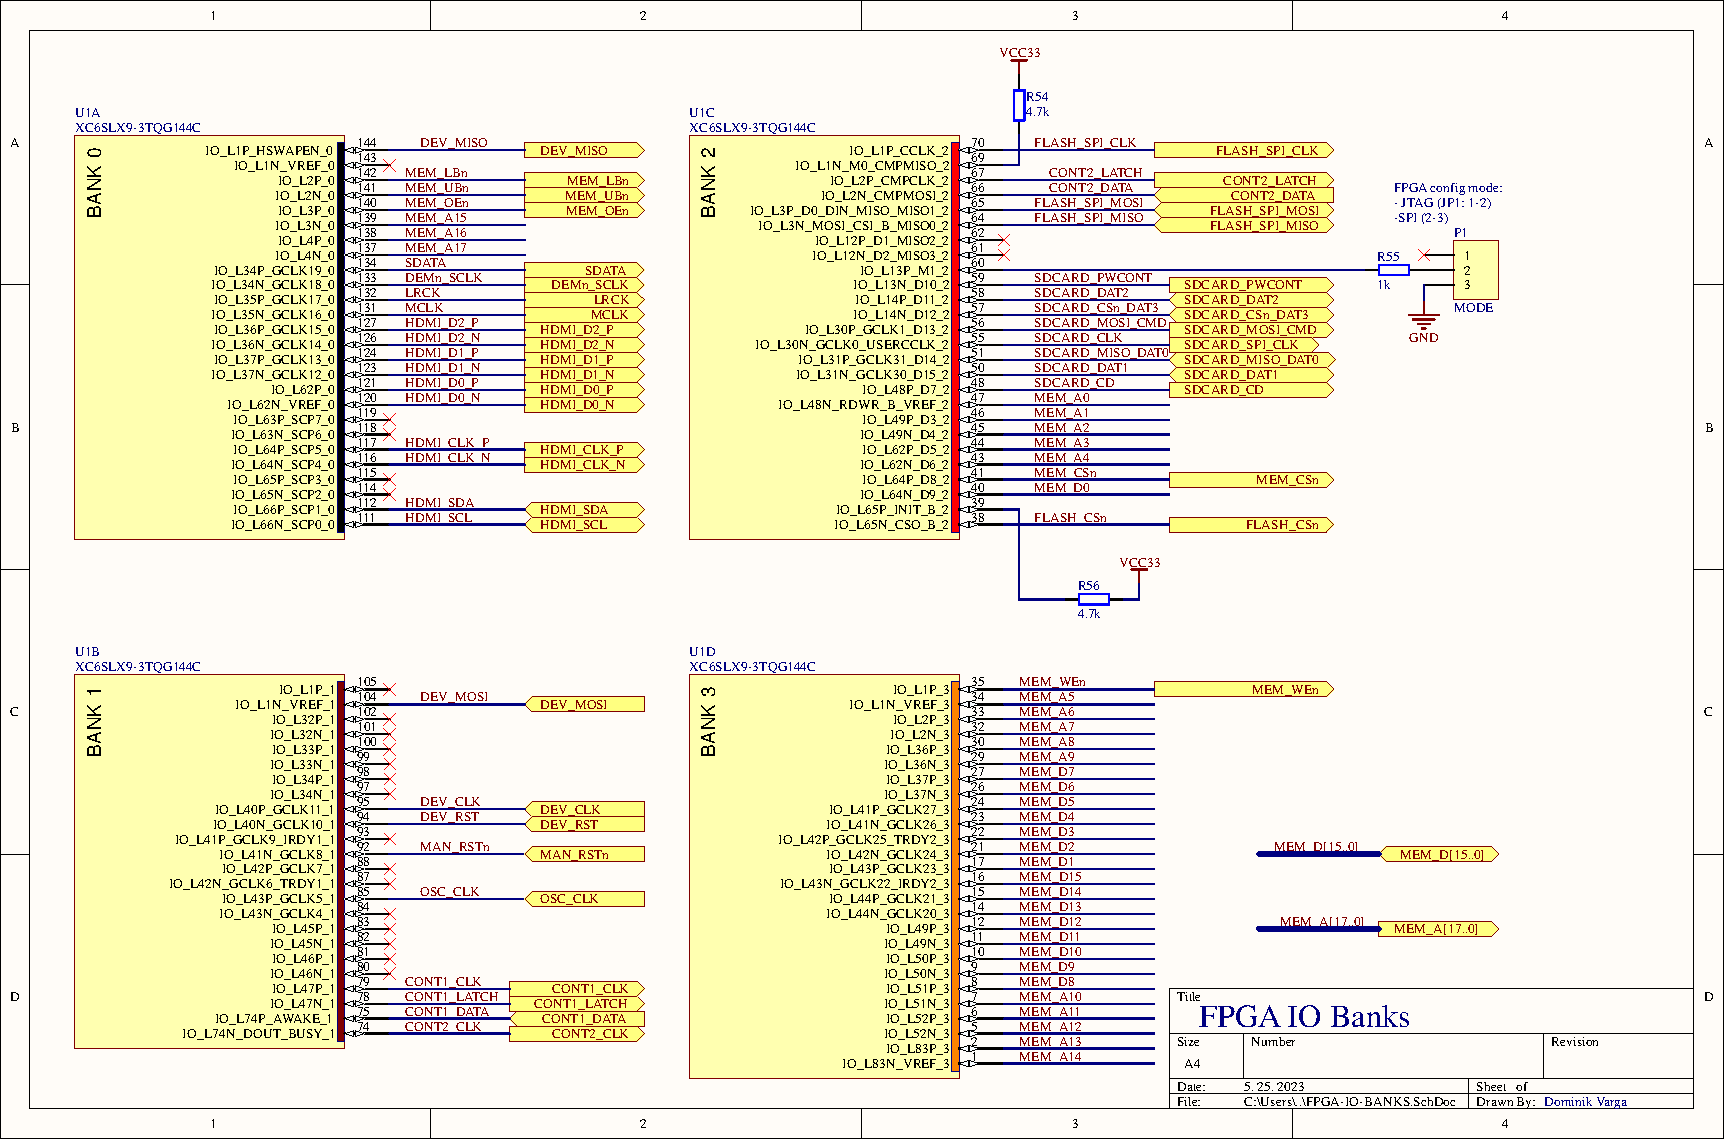
\includegraphics[width=220mm, keepaspectratio, angle=90]{figures/FPGA-BANKS}
	%\caption{FPGA IO bankok} 
	\label{fig:FPGA-BANKS}
\end{figure}


%\label{page:last}
\end{document}
